\documentclass[8pt,aspectratio=169]{beamer}
\usetheme{Madrid}
\usepackage{graphicx,booktabs,adjustbox,multicol,amsmath,amssymb,listings,xcolor,colortbl}
\definecolor{mlblue}{RGB}{0,102,204}
\definecolor{mlpurple}{RGB}{51,51,178}
\definecolor{mllavender}{RGB}{173,173,224}
\definecolor{mllavender2}{RGB}{193,193,232}
\definecolor{mllavender3}{RGB}{204,204,235}
\definecolor{mllavender4}{RGB}{214,214,239}
\definecolor{mlorange}{RGB}{255,127,14}
\definecolor{mlgreen}{RGB}{44,160,44}
\definecolor{mlred}{RGB}{214,39,40}
\definecolor{mlgray}{RGB}{127,127,127}
% Solidity colors
\definecolor{solkeyword}{RGB}{0,102,153}
\definecolor{solstring}{RGB}{163,21,21}
\definecolor{solcomment}{RGB}{0,128,0}
\definecolor{solnumber}{RGB}{0,128,128}
\setbeamercolor{palette primary}{bg=mllavender3,fg=mlpurple}
\setbeamercolor{palette secondary}{bg=mllavender2,fg=mlpurple}
\setbeamercolor{palette tertiary}{bg=mllavender,fg=white}
\setbeamercolor{palette quaternary}{bg=mlpurple,fg=white}
\setbeamercolor{structure}{fg=mlpurple}
\setbeamercolor{title}{fg=mlpurple}
\setbeamercolor{frametitle}{fg=mlpurple,bg=mllavender3}
\setbeamercolor{block title}{bg=mllavender2,fg=mlpurple}
\setbeamercolor{block body}{bg=mllavender4,fg=black}
\setbeamertemplate{navigation symbols}{}
\setbeamertemplate{itemize items}[circle]
\setbeamersize{text margin left=5mm,text margin right=5mm}
\newcommand{\bottomnote}[1]{\vfill\vspace{-2mm}\textcolor{mllavender2}{\rule{\textwidth}{0.4pt}}\vspace{1mm}\footnotesize\textbf{#1}}
% Solidity language definition
\lstdefinelanguage{Solidity}{
  keywords={pragma, solidity, contract, function, public, private, external, internal, view, pure, payable, returns, return, if, else, for, while, mapping, address, uint, uint256, int, string, bool, bytes, bytes32, event, emit, modifier, require, constructor, memory, storage, calldata, msg, sender, value, this, new, delete, true, false, import, is, constant, override, virtual, interface, library, abstract, struct, enum, unchecked, assembly, abi, encode, decode, keccak256, receive, fallback},
  keywordstyle=\color{solkeyword}\bfseries,
  sensitive=true,
  comment=[l]{//},
  morecomment=[s]{/*}{*/},
  commentstyle=\color{solcomment}\ttfamily,
  stringstyle=\color{solstring}\ttfamily,
  morestring=[b]',
  morestring=[b]"
}
\lstset{language=Solidity,basicstyle=\ttfamily\scriptsize,breaklines=true,frame=single,backgroundcolor=\color{mllavender4},numbers=left,numberstyle=\tiny\color{mlgray},numbersep=5pt,tabsize=2,showstringspaces=false}
\usepackage{tikz,pgfplots}
\pgfplotsset{compat=1.18}
\usetikzlibrary{arrows.meta,positioning,shapes.geometric,calc,chains,decorations.pathmorphing,automata,fit}
\title{Stablecoins \& CBDCs: A Quantitative Deep Dive}
\subtitle{Standalone Technical Lecture}
\author{Prof.~Dr.~Joerg Osterrieder}
\institute{University Lecture Series}
\date{\today}
\begin{document}

%% ============================================================
%% SECTION 0: OPENING
%% ============================================================

% Frame 1: Title
\begin{frame}
\titlepage
\end{frame}

% Frame 2: Lecture Roadmap
\begin{frame}{Lecture Roadmap}
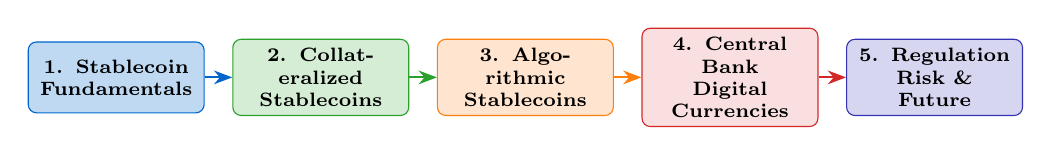
\begin{tikzpicture}[remember picture]
  \node[draw=mlblue, fill=mlblue!25, rounded corners=3pt, minimum width=2.1cm, minimum height=0.9cm, text width=2.0cm, align=center, font=\scriptsize\bfseries] (b1) {1. Stablecoin\\Fundamentals};
  \node[draw=mlgreen, fill=mlgreen!20, rounded corners=3pt, minimum width=2.1cm, minimum height=0.9cm, text width=2.0cm, align=center, font=\scriptsize\bfseries, right=0.35cm of b1] (b2) {2. Collateralized\\Stablecoins};
  \node[draw=mlorange, fill=mlorange!20, rounded corners=3pt, minimum width=2.1cm, minimum height=0.9cm, text width=2.0cm, align=center, font=\scriptsize\bfseries, right=0.35cm of b2] (b3) {3. Algorithmic\\Stablecoins};
  \node[draw=mlred, fill=mlred!15, rounded corners=3pt, minimum width=2.1cm, minimum height=0.9cm, text width=2.0cm, align=center, font=\scriptsize\bfseries, right=0.35cm of b3] (b4) {4. Central Bank\\Digital Currencies};
  \node[draw=mlpurple, fill=mlpurple!20, rounded corners=3pt, minimum width=2.1cm, minimum height=0.9cm, text width=2.0cm, align=center, font=\scriptsize\bfseries, right=0.35cm of b4] (b5) {5. Regulation\\Risk \& Future};
  \draw[-{Stealth}, thick, mlblue] (b1.east) -- (b2.west);
  \draw[-{Stealth}, thick, mlgreen] (b2.east) -- (b3.west);
  \draw[-{Stealth}, thick, mlorange] (b3.east) -- (b4.west);
  \draw[-{Stealth}, thick, mlred] (b4.east) -- (b5.west);
\end{tikzpicture}

\vspace{3mm}
\begin{columns}[T]
\column{0.5\textwidth}
\begin{block}{Learning Objectives}
\begin{itemize}\setlength{\itemsep}{1pt}
  \item Understand peg mechanisms and collateral models
  \item Analyse fiat-backed and crypto-backed designs
  \item Evaluate algorithmic stablecoin risks and failures
  \item Compare CBDC architectures and policy implications
  \item Apply quantitative risk metrics to stablecoin portfolios
\end{itemize}
\end{block}
\column{0.5\textwidth}
\begin{block}{Prerequisites}
\begin{itemize}\setlength{\itemsep}{1pt}
  \item Blockchain fundamentals (Lessons 1--2)
  \item Smart contract basics (Lessons 3--4)
  \item DeFi protocols overview (Lesson 5)
  \item Basic monetary economics
\end{itemize}
\end{block}
\end{columns}
\bottomnote{Duration: 90 minutes | 5 sections | \textasciitilde55 frames | Prerequisite: Lessons 1--4}
\end{frame}

% Frame 3: Table of Contents
\begin{frame}{Table of Contents}
\tableofcontents
\bottomnote{Navigate through 5 sections covering stablecoin fundamentals to CBDCs and regulation}
\end{frame}

%% ============================================================
%% SECTION 1: STABLECOIN FUNDAMENTALS
%% ============================================================
\section{Stablecoin Fundamentals}

% Frame 4: Section Divider
\begin{frame}{Section 1: Stablecoin Fundamentals}
\begin{beamercolorbox}[sep=12pt,center,rounded=true,shadow=true]{palette quaternary}
  {\Large\bfseries Section 1: Stablecoin Fundamentals}\\[4pt]
  {\normalsize Understanding price-stable digital assets and their role in the crypto ecosystem}
\end{beamercolorbox}

\vspace{4mm}
\begin{columns}[T]
\column{0.55\textwidth}
\begin{block}{What You Will Learn}
\begin{itemize}\setlength{\itemsep}{2pt}
  \item Why price stability matters in digital asset markets
  \item Core peg mechanisms: redemption, collateral, algorithms
  \item Taxonomy of stablecoin types and design trade-offs
  \item Market landscape: size, concentration, daily volumes
  \item Historical de-peg events and systemic risk
\end{itemize}
\end{block}
\column{0.45\textwidth}
\begin{block}{Frames in This Section}
\begin{itemize}\setlength{\itemsep}{2pt}
  \item Frame 5: The Volatility Problem
  \item Frame 6: What is a Stablecoin?
  \item Frame 7: Stablecoin Taxonomy
  \item Frame 8: Peg Mechanism Overview
  \item Frame 9: Market Landscape
  \item Frame 10: Market Share Chart
  \item Frame 11: Use Cases
  \item Frame 12: De-Peg Events Timeline
  \item Frame 13: Volume vs.\ TradFi
  \item Frame 14: Section Summary
\end{itemize}
\end{block}
\end{columns}
\bottomnote{Section 1 of 5 | Frames 4--14 | Foundational concepts before technical deep dives}
\end{frame}

% Frame 5: The Volatility Problem
\begin{frame}{The Volatility Problem}
\begin{columns}[T]
\column{0.44\textwidth}
\begin{block}{Why Volatility Breaks Money}
\begin{itemize}\setlength{\itemsep}{2pt}
  \item \textbf{Store of value:} BTC lost 80\% in 2018, 75\% in 2022 --- unusable savings
  \item \textbf{Unit of account:} Prices denominated in BTC change daily; merchants cannot plan
  \item \textbf{Medium of exchange:} A \$5 coffee may cost 0.00008 BTC today and 0.00012 BTC tomorrow
  \item \textbf{Annualised volatility:} BTC $\approx$70--80\%; USD $<$1\%; EUR $\approx$7\%
  \item \textbf{Consequence:} DeFi protocols need a stable unit for loans, collateral, and settlement
\end{itemize}
\end{block}
\vspace{2mm}
\begin{alertblock}{Key Insight}
\scriptsize Stablecoins decouple blockchain utility from crypto market volatility, enabling predictable financial applications.
\end{alertblock}
\column{0.56\textwidth}
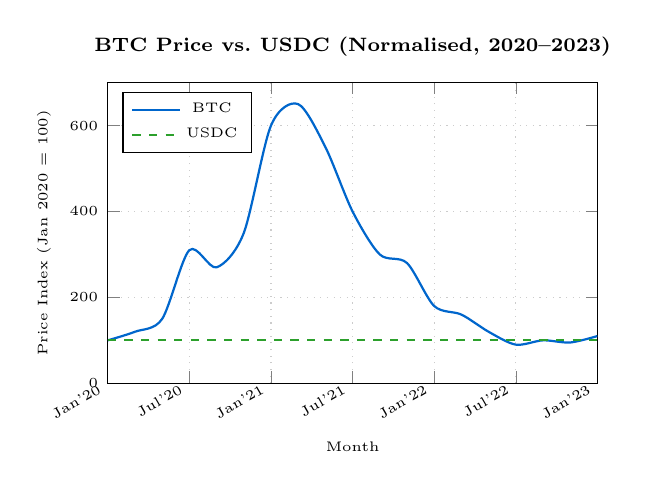
\begin{tikzpicture}
\begin{axis}[
  width=7.8cm, height=5.4cm,
  title={\scriptsize\bfseries BTC Price vs.\ USDC (Normalised, 2020--2023)},
  xlabel={\tiny Month},
  ylabel={\tiny Price Index (Jan 2020 = 100)},
  xmin=0, xmax=36,
  ymin=0, ymax=700,
  xtick={0,6,12,18,24,30,36},
  xticklabels={\tiny Jan'20,\tiny Jul'20,\tiny Jan'21,\tiny Jul'21,\tiny Jan'22,\tiny Jul'22,\tiny Jan'23},
  xticklabel style={rotate=30,anchor=east,font=\tiny},
  yticklabel style={font=\tiny},
  legend pos=north west,
  legend style={font=\tiny},
  grid=major,
  grid style={dotted,mlgray!40},
  title style={font=\scriptsize},
  xlabel style={font=\tiny},
  ylabel style={font=\tiny}
]
\addplot[thick, mlblue, smooth] coordinates {
  (0,100)(2,120)(4,150)(6,310)(8,270)(10,350)(12,600)(14,650)(16,550)(18,400)(20,300)(22,280)(24,180)(26,160)(28,120)(30,90)(32,100)(34,95)(36,110)
};
\addplot[thick, mlgreen, dashed] coordinates {
  (0,100)(6,100)(12,100)(18,100)(24,100)(30,100)(36,100)
};
\legend{BTC, USDC}
\end{axis}
\end{tikzpicture}
\end{columns}
\bottomnote{BTC annualised volatility source: CoinMetrics 2023 | USDC maintains \$1 peg within $\pm$0.1\% under normal conditions}
\end{frame}

% Frame 6: What is a Stablecoin?
\begin{frame}{What is a Stablecoin?}
\begin{columns}[T]
\column{0.48\textwidth}
\begin{block}{Definition}
A \textbf{stablecoin} is a cryptographic token designed to maintain a stable value relative to a reference asset (peg), typically a fiat currency (USD, EUR), a commodity (gold), or a basket of assets.
\end{block}
\vspace{2mm}
\begin{block}{Core Properties}
\begin{itemize}\setlength{\itemsep}{2pt}
  \item \textbf{Price stability:} Minimise deviation from peg ($|\Delta p| < \epsilon$)
  \item \textbf{Redeemability:} Holders can exchange tokens for underlying value
  \item \textbf{Scalability:} Supply adjusts to demand without destabilising peg
  \item \textbf{Decentralisation (optional):} Some designs avoid single issuer
  \item \textbf{Transparency:} Reserve composition verifiable by holders
\end{itemize}
\end{block}
\vspace{2mm}
\begin{alertblock}{Formal Peg Condition}
\scriptsize $\forall t:\; |P_t - P^* | < \delta$ \quad where $P^*$ is the target price and $\delta$ is the tolerance band (typically \$0.005 for USD stablecoins)
\end{alertblock}
\column{0.52\textwidth}
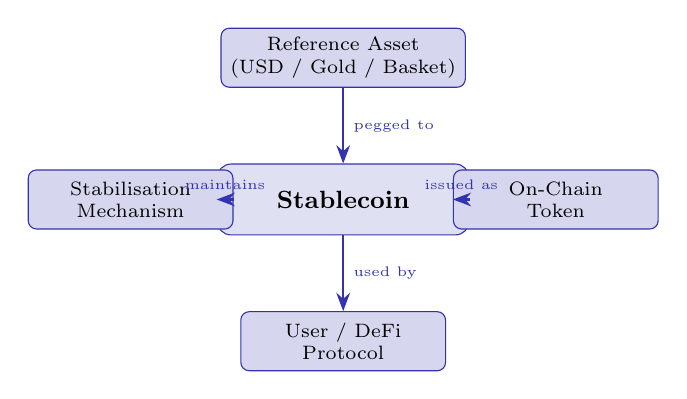
\begin{tikzpicture}[
  box/.style={draw=mlpurple, fill=mllavender4, rounded corners=3pt, minimum width=2.6cm, minimum height=0.75cm, align=center, font=\scriptsize},
  arrow/.style={-{Stealth}, thick, mlpurple}
]
  \node[draw=mlpurple, fill=mlpurple!15, rounded corners=5pt, minimum width=3.2cm, minimum height=0.9cm, align=center, font=\small\bfseries] (center) at (3.2,3.2) {Stablecoin};
  \node[box] (ref) at (3.2,5.0) {Reference Asset\\(USD / Gold / Basket)};
  \node[box] (mech) at (0.5,3.2) {Stabilisation\\Mechanism};
  \node[box] (token) at (5.9,3.2) {On-Chain\\Token};
  \node[box] (user) at (3.2,1.4) {User / DeFi\\Protocol};
  \draw[arrow] (ref.south) -- (center.north) node[midway,right,font=\tiny] {pegged to};
  \draw[arrow] (mech.east) -- (center.west) node[midway,above,font=\tiny] {maintains};
  \draw[arrow] (center.east) -- (token.west) node[midway,above,font=\tiny] {issued as};
  \draw[arrow] (center.south) -- (user.north) node[midway,right,font=\tiny] {used by};
\end{tikzpicture}
\end{columns}
\bottomnote{Stablecoins bridge traditional finance and DeFi | \$130B+ total market cap as of 2023 | Critical infrastructure for crypto markets}
\end{frame}

% Frame 7: Stablecoin Taxonomy
\begin{frame}{Stablecoin Taxonomy}
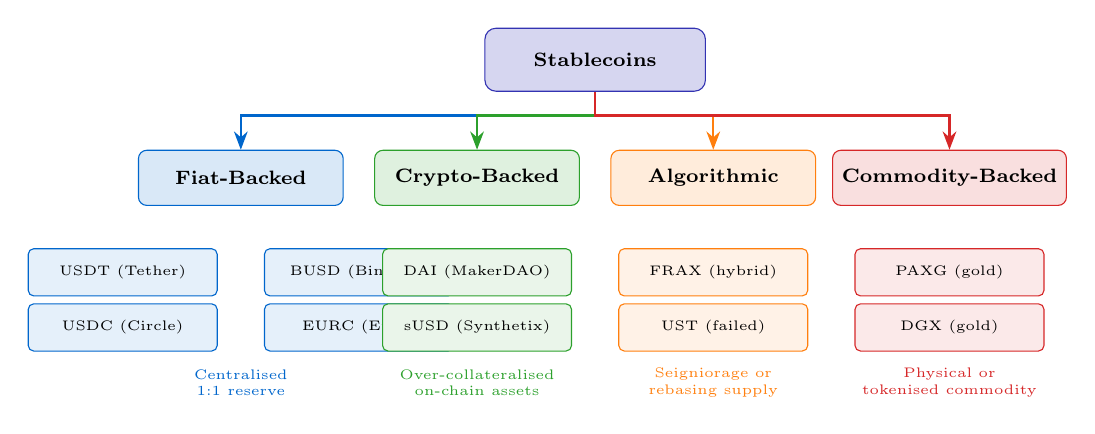
\begin{tikzpicture}[
  root/.style={draw=mlpurple, fill=mlpurple!20, rounded corners=4pt, minimum width=2.8cm, minimum height=0.8cm, align=center, font=\scriptsize\bfseries}
]
  \node[root] (sc) at (6.0,4.5) {Stablecoins};

  \node[draw=mlblue, fill=mlblue!15, rounded corners=3pt, minimum width=2.6cm, minimum height=0.7cm, align=center, font=\scriptsize\bfseries] (fiat) at (1.5,3.0) {Fiat-Backed};
  \node[draw=mlgreen, fill=mlgreen!15, rounded corners=3pt, minimum width=2.6cm, minimum height=0.7cm, align=center, font=\scriptsize\bfseries] (crypto) at (4.5,3.0) {Crypto-Backed};
  \node[draw=mlorange, fill=mlorange!15, rounded corners=3pt, minimum width=2.6cm, minimum height=0.7cm, align=center, font=\scriptsize\bfseries] (algo) at (7.5,3.0) {Algorithmic};
  \node[draw=mlred, fill=mlred!15, rounded corners=3pt, minimum width=2.6cm, minimum height=0.7cm, align=center, font=\scriptsize\bfseries] (comm) at (10.5,3.0) {Commodity-Backed};

  \draw[-{Stealth}, thick, mlblue] (sc.south) -- ++(0,-0.3) -| (fiat.north);
  \draw[-{Stealth}, thick, mlgreen] (sc.south) -- ++(0,-0.3) -| (crypto.north);
  \draw[-{Stealth}, thick, mlorange] (sc.south) -- ++(0,-0.3) -| (algo.north);
  \draw[-{Stealth}, thick, mlred] (sc.south) -- ++(0,-0.3) -| (comm.north);

  \node[draw=mlblue, fill=mlblue!10, rounded corners=2pt, minimum width=2.4cm, minimum height=0.6cm, align=center, font=\tiny] at (0.0,1.8) {USDT (Tether)};
  \node[draw=mlblue, fill=mlblue!10, rounded corners=2pt, minimum width=2.4cm, minimum height=0.6cm, align=center, font=\tiny] at (0.0,1.1) {USDC (Circle)};
  \node[draw=mlblue, fill=mlblue!10, rounded corners=2pt, minimum width=2.4cm, minimum height=0.6cm, align=center, font=\tiny] at (3.0,1.8) {BUSD (Binance)};
  \node[draw=mlblue, fill=mlblue!10, rounded corners=2pt, minimum width=2.4cm, minimum height=0.6cm, align=center, font=\tiny] at (3.0,1.1) {EURC (Euro)};

  \node[draw=mlgreen, fill=mlgreen!10, rounded corners=2pt, minimum width=2.4cm, minimum height=0.6cm, align=center, font=\tiny] at (4.5,1.8) {DAI (MakerDAO)};
  \node[draw=mlgreen, fill=mlgreen!10, rounded corners=2pt, minimum width=2.4cm, minimum height=0.6cm, align=center, font=\tiny] at (4.5,1.1) {sUSD (Synthetix)};

  \node[draw=mlorange, fill=mlorange!10, rounded corners=2pt, minimum width=2.4cm, minimum height=0.6cm, align=center, font=\tiny] at (7.5,1.8) {FRAX (hybrid)};
  \node[draw=mlorange, fill=mlorange!10, rounded corners=2pt, minimum width=2.4cm, minimum height=0.6cm, align=center, font=\tiny] at (7.5,1.1) {UST (failed)};

  \node[draw=mlred, fill=mlred!10, rounded corners=2pt, minimum width=2.4cm, minimum height=0.6cm, align=center, font=\tiny] at (10.5,1.8) {PAXG (gold)};
  \node[draw=mlred, fill=mlred!10, rounded corners=2pt, minimum width=2.4cm, minimum height=0.6cm, align=center, font=\tiny] at (10.5,1.1) {DGX (gold)};

  \node[font=\tiny, text=mlblue, align=center] at (1.5,0.4) {Centralised\\1:1 reserve};
  \node[font=\tiny, text=mlgreen, align=center] at (4.5,0.4) {Over-collateralised\\on-chain assets};
  \node[font=\tiny, text=mlorange, align=center] at (7.5,0.4) {Seigniorage or\\rebasing supply};
  \node[font=\tiny, text=mlred, align=center] at (10.5,0.4) {Physical or\\tokenised commodity};
\end{tikzpicture}
\bottomnote{Four primary design categories | Fiat-backed dominates with $>$85\% market share | Each category presents distinct risk--trust trade-offs}
\end{frame}

% Frame 8: Peg Mechanism Overview
\begin{frame}{Peg Mechanism Overview}
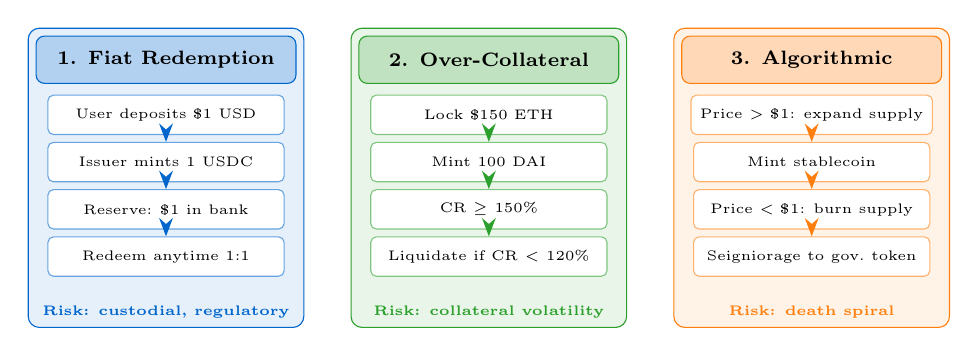
\begin{tikzpicture}
  % Panel 1: Redemption
  \node[draw=mlblue, fill=mlblue!10, rounded corners=4pt, minimum width=3.5cm, minimum height=3.8cm, align=center] (p1) at (1.9,2.0) {};
  \node[draw=mlblue, fill=mlblue!30, rounded corners=3pt, minimum width=3.3cm, minimum height=0.6cm, align=center, font=\scriptsize\bfseries] at (1.9,3.5) {1. Fiat Redemption};
  \node[draw=mlblue!60, fill=white, rounded corners=2pt, minimum width=3.0cm, minimum height=0.5cm, align=center, font=\tiny] (s1a) at (1.9,2.8) {User deposits \$1 USD};
  \node[draw=mlblue!60, fill=white, rounded corners=2pt, minimum width=3.0cm, minimum height=0.5cm, align=center, font=\tiny] (s1b) at (1.9,2.2) {Issuer mints 1 USDC};
  \node[draw=mlblue!60, fill=white, rounded corners=2pt, minimum width=3.0cm, minimum height=0.5cm, align=center, font=\tiny] (s1c) at (1.9,1.6) {Reserve: \$1 in bank};
  \node[draw=mlblue!60, fill=white, rounded corners=2pt, minimum width=3.0cm, minimum height=0.5cm, align=center, font=\tiny] (s1d) at (1.9,1.0) {Redeem anytime 1:1};
  \draw[-{Stealth}, thick, mlblue] (s1a.south) -- (s1b.north);
  \draw[-{Stealth}, thick, mlblue] (s1b.south) -- (s1c.north);
  \draw[-{Stealth}, thick, mlblue] (s1c.south) -- (s1d.north);

  % Panel 2: Over-collateralisation
  \node[draw=mlgreen, fill=mlgreen!10, rounded corners=4pt, minimum width=3.5cm, minimum height=3.8cm, align=center] (p2) at (6.0,2.0) {};
  \node[draw=mlgreen, fill=mlgreen!30, rounded corners=3pt, minimum width=3.3cm, minimum height=0.6cm, align=center, font=\scriptsize\bfseries] at (6.0,3.5) {2. Over-Collateral};
  \node[draw=mlgreen!60, fill=white, rounded corners=2pt, minimum width=3.0cm, minimum height=0.5cm, align=center, font=\tiny] (s2a) at (6.0,2.8) {Lock \$150 ETH};
  \node[draw=mlgreen!60, fill=white, rounded corners=2pt, minimum width=3.0cm, minimum height=0.5cm, align=center, font=\tiny] (s2b) at (6.0,2.2) {Mint 100 DAI};
  \node[draw=mlgreen!60, fill=white, rounded corners=2pt, minimum width=3.0cm, minimum height=0.5cm, align=center, font=\tiny] (s2c) at (6.0,1.6) {CR $\geq$ 150\%};
  \node[draw=mlgreen!60, fill=white, rounded corners=2pt, minimum width=3.0cm, minimum height=0.5cm, align=center, font=\tiny] (s2d) at (6.0,1.0) {Liquidate if CR $<$ 120\%};
  \draw[-{Stealth}, thick, mlgreen] (s2a.south) -- (s2b.north);
  \draw[-{Stealth}, thick, mlgreen] (s2b.south) -- (s2c.north);
  \draw[-{Stealth}, thick, mlgreen] (s2c.south) -- (s2d.north);

  % Panel 3: Algorithmic
  \node[draw=mlorange, fill=mlorange!10, rounded corners=4pt, minimum width=3.5cm, minimum height=3.8cm, align=center] (p3) at (10.1,2.0) {};
  \node[draw=mlorange, fill=mlorange!30, rounded corners=3pt, minimum width=3.3cm, minimum height=0.6cm, align=center, font=\scriptsize\bfseries] at (10.1,3.5) {3. Algorithmic};
  \node[draw=mlorange!60, fill=white, rounded corners=2pt, minimum width=3.0cm, minimum height=0.5cm, align=center, font=\tiny] (s3a) at (10.1,2.8) {Price $>$ \$1: expand supply};
  \node[draw=mlorange!60, fill=white, rounded corners=2pt, minimum width=3.0cm, minimum height=0.5cm, align=center, font=\tiny] (s3b) at (10.1,2.2) {Mint stablecoin};
  \node[draw=mlorange!60, fill=white, rounded corners=2pt, minimum width=3.0cm, minimum height=0.5cm, align=center, font=\tiny] (s3c) at (10.1,1.6) {Price $<$ \$1: burn supply};
  \node[draw=mlorange!60, fill=white, rounded corners=2pt, minimum width=3.0cm, minimum height=0.5cm, align=center, font=\tiny] (s3d) at (10.1,1.0) {Seigniorage to gov.\ token};
  \draw[-{Stealth}, thick, mlorange] (s3a.south) -- (s3b.north);
  \draw[-{Stealth}, thick, mlorange] (s3b.south) -- (s3c.north);
  \draw[-{Stealth}, thick, mlorange] (s3c.south) -- (s3d.north);

  \node[font=\tiny\bfseries, text=mlblue] at (1.9,0.3) {Risk: custodial, regulatory};
  \node[font=\tiny\bfseries, text=mlgreen] at (6.0,0.3) {Risk: collateral volatility};
  \node[font=\tiny\bfseries, text=mlorange] at (10.1,0.3) {Risk: death spiral};
\end{tikzpicture}
\bottomnote{Collateralisation ratio (CR) = collateral value / stablecoin value | Algorithmic designs depend on reflexive demand assumptions}
\end{frame}

% Frame 9: Stablecoin Market Landscape
\begin{frame}{Stablecoin Market Landscape}
\begin{columns}[T]
\column{0.55\textwidth}
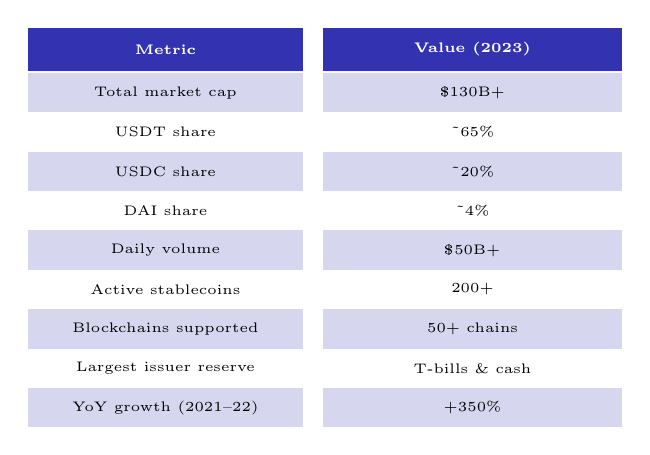
\begin{tikzpicture}[
  hdr/.style={fill=mlpurple, text=white, font=\tiny\bfseries, minimum height=0.55cm, align=center},
  row1/.style={fill=mllavender4, font=\tiny, minimum height=0.50cm, align=center},
  row2/.style={fill=white, font=\tiny, minimum height=0.50cm, align=center}
]
  \node[hdr, minimum width=3.5cm] at (1.75,5.8) {Metric};
  \node[hdr, minimum width=3.8cm] at (5.65,5.8) {Value (2023)};

  \node[row1, minimum width=3.5cm] at (1.75,5.25) {Total market cap};
  \node[row1, minimum width=3.8cm] at (5.65,5.25) {\$130B+};

  \node[row2, minimum width=3.5cm] at (1.75,4.75) {USDT share};
  \node[row2, minimum width=3.8cm] at (5.65,4.75) {\textasciitilde65\%};

  \node[row1, minimum width=3.5cm] at (1.75,4.25) {USDC share};
  \node[row1, minimum width=3.8cm] at (5.65,4.25) {\textasciitilde20\%};

  \node[row2, minimum width=3.5cm] at (1.75,3.75) {DAI share};
  \node[row2, minimum width=3.8cm] at (5.65,3.75) {\textasciitilde4\%};

  \node[row1, minimum width=3.5cm] at (1.75,3.25) {Daily volume};
  \node[row1, minimum width=3.8cm] at (5.65,3.25) {\$50B+};

  \node[row2, minimum width=3.5cm] at (1.75,2.75) {Active stablecoins};
  \node[row2, minimum width=3.8cm] at (5.65,2.75) {200+};

  \node[row1, minimum width=3.5cm] at (1.75,2.25) {Blockchains supported};
  \node[row1, minimum width=3.8cm] at (5.65,2.25) {50+ chains};

  \node[row2, minimum width=3.5cm] at (1.75,1.75) {Largest issuer reserve};
  \node[row2, minimum width=3.8cm] at (5.65,1.75) {T-bills \& cash};

  \node[row1, minimum width=3.5cm] at (1.75,1.25) {YoY growth (2021--22)};
  \node[row1, minimum width=3.8cm] at (5.65,1.25) {+350\%};
\end{tikzpicture}
\column{0.45\textwidth}
\begin{block}{Market Significance}
\begin{itemize}\setlength{\itemsep}{2pt}
  \item Stablecoins now exceed \textbf{10\% of total crypto market cap}
  \item USDT daily volume rivals Visa on peak days
  \item Critical settlement layer for CEX and DEX trading
  \item Primary vehicle for DeFi liquidity provision
  \item Tether reserves include US Treasury bills, making it a significant holder
\end{itemize}
\end{block}
\vspace{2mm}
\begin{alertblock}{Concentration Risk}
\scriptsize Top 2 stablecoins (USDT + USDC) control $>$85\% of market. Systemic failure of either would cascade across all of DeFi and centralised exchanges.
\end{alertblock}
\end{columns}
\bottomnote{Data: CoinGecko, DefiLlama Q3 2023 | USDT issued by Tether Ltd (BVI) | USDC issued by Circle (US-regulated)}
\end{frame}

% Frame 10: Stablecoin Market Share Chart
\begin{frame}{Stablecoin Market Share Chart}
\begin{columns}[T]
\column{0.58\textwidth}
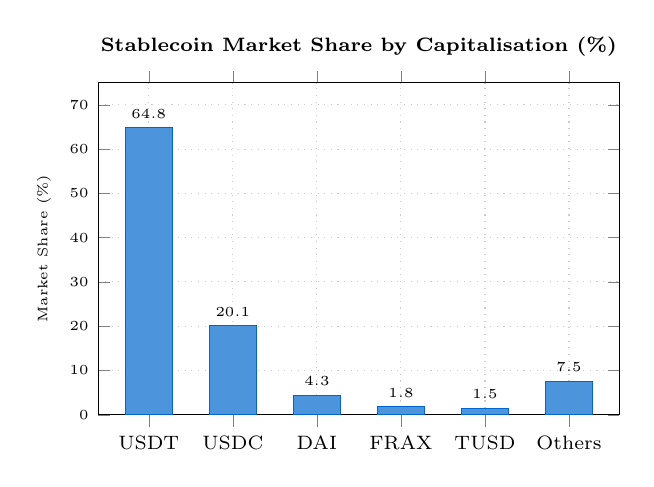
\begin{tikzpicture}
\begin{axis}[
  width=8.2cm, height=5.8cm,
  title={\scriptsize\bfseries Stablecoin Market Share by Capitalisation (\%)},
  ybar,
  bar width=0.6cm,
  symbolic x coords={USDT, USDC, DAI, FRAX, TUSD, Others},
  xtick=data,
  xticklabel style={font=\scriptsize},
  yticklabel style={font=\tiny},
  ylabel={\tiny Market Share (\%)},
  ymin=0, ymax=75,
  ytick={0,10,20,30,40,50,60,70},
  nodes near coords,
  nodes near coords style={font=\tiny, anchor=south},
  grid=major,
  grid style={dotted, mlgray!40},
  title style={font=\scriptsize},
  ylabel style={font=\tiny},
  enlarge x limits=0.12
]
\addplot[fill=mlblue!70, draw=mlblue] coordinates {
  (USDT,64.8) (USDC,20.1) (DAI,4.3) (FRAX,1.8) (TUSD,1.5) (Others,7.5)
};
\end{axis}
\end{tikzpicture}
\column{0.42\textwidth}
\begin{block}{Key Observations}
\begin{itemize}\setlength{\itemsep}{3pt}
  \item \textbf{USDT dominance:} 64.8\% despite repeated audit controversies
  \item \textbf{USDC growth:} Regulatory clarity driving institutional adoption
  \item \textbf{DAI resilience:} Survived 2022 crypto winter via over-collateralisation
  \item \textbf{FRAX hybrid:} Partial algorithmic design reduced risk vs.\ pure-algo
  \item \textbf{Long tail:} 200+ stablecoins share remaining 7.5\%
\end{itemize}
\end{block}
\vspace{2mm}
\begin{block}{Herfindahl--Hirschman Index}
\scriptsize $\text{HHI} = \sum_i s_i^2 \approx 0.648^2 + 0.201^2 + \ldots \approx 0.465$\\
Very high concentration (HHI $>$ 0.25 = highly concentrated)
\end{block}
\end{columns}
\bottomnote{Source: CoinGecko November 2023 | HHI $>$ 0.25 indicates highly concentrated market | TUSD = TrueUSD}
\end{frame}

% Frame 11: Stablecoin Use Cases
\begin{frame}{Stablecoin Use Cases}
\begin{columns}[T]
\column{0.52\textwidth}
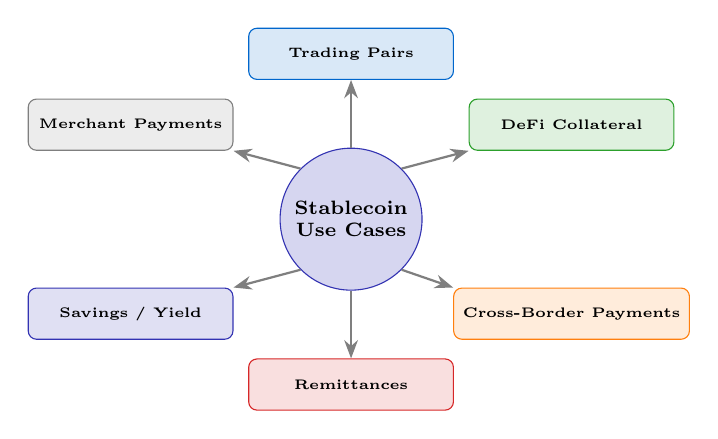
\begin{tikzpicture}[
  hub/.style={draw=mlpurple, fill=mlpurple!20, circle, minimum size=1.8cm, align=center, font=\scriptsize\bfseries}
]
  \node[hub] (center) at (3.5,3.2) {Stablecoin\\Use Cases};

  \node[draw=mlblue, fill=mlblue!15, rounded corners=3pt, minimum width=2.6cm, minimum height=0.65cm, align=center, font=\tiny\bfseries] (t1) at (3.5,5.3) {Trading Pairs};
  \node[draw=mlgreen, fill=mlgreen!15, rounded corners=3pt, minimum width=2.6cm, minimum height=0.65cm, align=center, font=\tiny\bfseries] (t2) at (6.3,4.4) {DeFi Collateral};
  \node[draw=mlorange, fill=mlorange!15, rounded corners=3pt, minimum width=2.6cm, minimum height=0.65cm, align=center, font=\tiny\bfseries] (t3) at (6.3,2.0) {Cross-Border Payments};
  \node[draw=mlred, fill=mlred!15, rounded corners=3pt, minimum width=2.6cm, minimum height=0.65cm, align=center, font=\tiny\bfseries] (t4) at (3.5,1.1) {Remittances};
  \node[draw=mlpurple, fill=mlpurple!15, rounded corners=3pt, minimum width=2.6cm, minimum height=0.65cm, align=center, font=\tiny\bfseries] (t5) at (0.7,2.0) {Savings / Yield};
  \node[draw=mlgray, fill=mlgray!15, rounded corners=3pt, minimum width=2.6cm, minimum height=0.65cm, align=center, font=\tiny\bfseries] (t6) at (0.7,4.4) {Merchant Payments};

  \draw[-{Stealth}, thick, mlgray] (center.north) -- (t1.south);
  \draw[-{Stealth}, thick, mlgray] (center.north east) -- (t2.south west);
  \draw[-{Stealth}, thick, mlgray] (center.south east) -- (t3.north west);
  \draw[-{Stealth}, thick, mlgray] (center.south) -- (t4.north);
  \draw[-{Stealth}, thick, mlgray] (center.south west) -- (t5.north east);
  \draw[-{Stealth}, thick, mlgray] (center.north west) -- (t6.south east);
\end{tikzpicture}
\column{0.48\textwidth}
\begin{block}{Use Case Details}
\begin{itemize}\setlength{\itemsep}{2pt}
  \item \textbf{Trading pairs:} BTC/USDT is the most-traded pair globally; avoids fiat withdrawal
  \item \textbf{DeFi collateral:} Aave, Compound accept USDC as highest-quality collateral
  \item \textbf{Cross-border:} Stellar USDC settles in 5s vs.\ 2--5 days SWIFT
  \item \textbf{Remittances:} MoneyGram--Stellar partnership; fees $<$1\% vs.\ Western Union 5--8\%
  \item \textbf{Savings/yield:} Anchor Protocol offered 20\% APY (unsustainably; collapsed 2022)
  \item \textbf{Merchant:} Shopify, PayPal, Stripe now support USDC settlement
\end{itemize}
\end{block}
\vspace{1mm}
\begin{alertblock}{Emerging Use: CBDCs}
\scriptsize Central banks are building their own stablecoins; retail CBDC pilots running in 130+ countries
\end{alertblock}
\end{columns}
\bottomnote{Stablecoins processed \$7.4T in on-chain volume in 2022 (Visa processed \$14T globally) | Fastest-growing payment rail in emerging markets}
\end{frame}

% Frame 12: De-Peg Events Timeline
\begin{frame}{De-Peg Events Timeline}
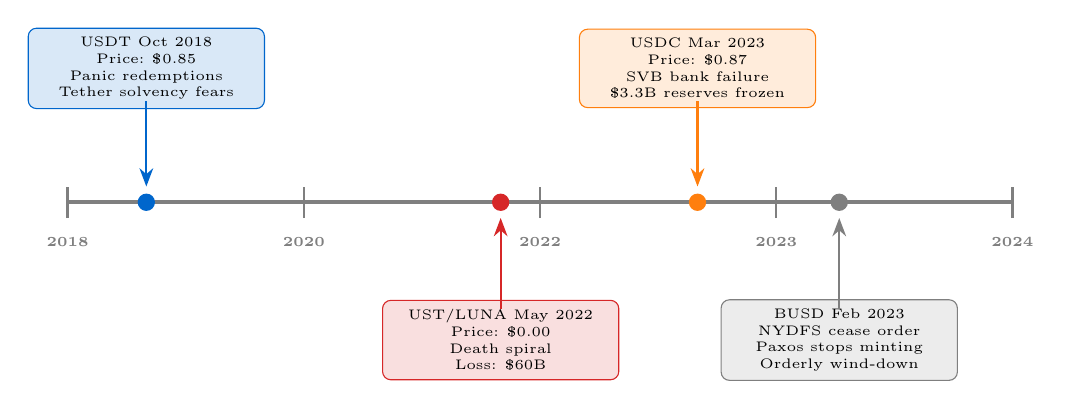
\begin{tikzpicture}
  % Timeline axis
  \draw[draw=mlgray, line width=1.5pt] (0,2.8) -- (12.0,2.8);
  \foreach \x in {0,3,6,9,12} \draw[mlgray, line width=0.8pt] (\x,2.6) -- (\x,3.0);
  \node[font=\tiny\bfseries, text=mlgray] at (0,2.3) {2018};
  \node[font=\tiny\bfseries, text=mlgray] at (3,2.3) {2020};
  \node[font=\tiny\bfseries, text=mlgray] at (6,2.3) {2022};
  \node[font=\tiny\bfseries, text=mlgray] at (9,2.3) {2023};
  \node[font=\tiny\bfseries, text=mlgray] at (12,2.3) {2024};

  % Event 1: USDT 2018
  \node[circle, fill=mlblue, minimum size=0.22cm, inner sep=0pt] at (1.0,2.8) {};
  \node[draw=mlblue, fill=mlblue!15, rounded corners=3pt, minimum width=3.0cm, minimum height=0.9cm, align=center, font=\tiny] at (1.0,4.5) {USDT Oct 2018\\Price: \$0.85\\Panic redemptions\\Tether solvency fears};
  \draw[-{Stealth}, thick, mlblue] (1.0,4.08) -- (1.0,3.0);

  % Event 2: UST/LUNA 2022
  \node[circle, fill=mlred, minimum size=0.22cm, inner sep=0pt] at (5.5,2.8) {};
  \node[draw=mlred, fill=mlred!15, rounded corners=3pt, minimum width=3.0cm, minimum height=0.9cm, align=center, font=\tiny] at (5.5,1.05) {UST/LUNA May 2022\\Price: \$0.00\\Death spiral\\Loss: \$60B};
  \draw[-{Stealth}, thick, mlred] (5.5,1.45) -- (5.5,2.6);

  % Event 3: USDC SVB 2023
  \node[circle, fill=mlorange, minimum size=0.22cm, inner sep=0pt] at (8.0,2.8) {};
  \node[draw=mlorange, fill=mlorange!15, rounded corners=3pt, minimum width=3.0cm, minimum height=0.9cm, align=center, font=\tiny] at (8.0,4.5) {USDC Mar 2023\\Price: \$0.87\\SVB bank failure\\\$3.3B reserves frozen};
  \draw[-{Stealth}, thick, mlorange] (8.0,4.08) -- (8.0,3.0);

  % Event 4: BUSD 2023
  \node[circle, fill=mlgray, minimum size=0.22cm, inner sep=0pt] at (9.8,2.8) {};
  \node[draw=mlgray, fill=mlgray!15, rounded corners=3pt, minimum width=3.0cm, minimum height=0.9cm, align=center, font=\tiny] at (9.8,1.05) {BUSD Feb 2023\\NYDFS cease order\\Paxos stops minting\\Orderly wind-down};
  \draw[-{Stealth}, thick, mlgray] (9.8,1.45) -- (9.8,2.6);
\end{tikzpicture}
\bottomnote{UST/LUNA collapse (May 2022) is the largest stablecoin failure in history | USDC SVB de-peg recovered within 48 hours after US Treasury intervention}
\end{frame}

% Frame 13: Transaction Volume vs Traditional Finance
\begin{frame}{Transaction Volume vs.\ Traditional Finance}
\begin{columns}[T]
\column{0.58\textwidth}
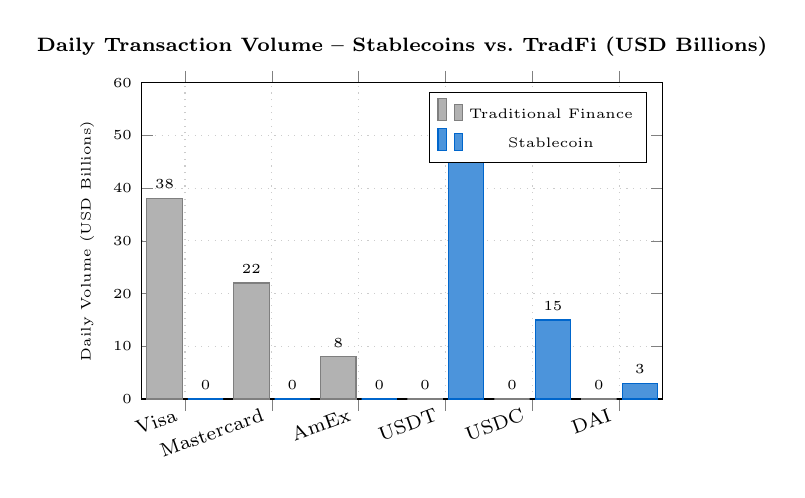
\begin{tikzpicture}
\begin{axis}[
  width=8.2cm, height=5.6cm,
  title={\scriptsize\bfseries Daily Transaction Volume -- Stablecoins vs.\ TradFi (USD Billions)},
  ybar,
  bar width=0.45cm,
  symbolic x coords={Visa, Mastercard, AmEx, USDT, USDC, DAI},
  xtick=data,
  xticklabel style={font=\scriptsize, rotate=20, anchor=east},
  yticklabel style={font=\tiny},
  ylabel={\tiny Daily Volume (USD Billions)},
  ymin=0, ymax=60,
  ytick={0,10,20,30,40,50,60},
  nodes near coords,
  nodes near coords style={font=\tiny, anchor=south},
  grid=major,
  grid style={dotted, mlgray!40},
  title style={font=\scriptsize},
  ylabel style={font=\tiny},
  enlarge x limits=0.1,
  legend pos=north east,
  legend style={font=\tiny}
]
\addplot[fill=mlgray!60, draw=mlgray] coordinates {
  (Visa,38.0) (Mastercard,22.0) (AmEx,8.0) (USDT,0) (USDC,0) (DAI,0)
};
\addplot[fill=mlblue!70, draw=mlblue] coordinates {
  (Visa,0) (Mastercard,0) (AmEx,0) (USDT,50.0) (USDC,15.0) (DAI,3.0)
};
\legend{Traditional Finance, Stablecoin}
\end{axis}
\end{tikzpicture}
\column{0.42\textwidth}
\begin{block}{Volume Analysis}
\begin{itemize}\setlength{\itemsep}{2pt}
  \item \textbf{USDT surpasses Visa:} On peak days, USDT processes $>$\$50B vs.\ Visa's \$38B average
  \item \textbf{Settlement finality:} Stablecoin transfers settle in seconds; Visa settles in 1--3 days
  \item \textbf{Cost:} USDT transfer on Tron: \$0.001; Visa merchant fee: 1.5--3.5\%
  \item \textbf{Geography:} Stablecoins dominant in EM (Turkey, Argentina, Vietnam)
\end{itemize}
\end{block}
\vspace{2mm}
\begin{block}{Settlement Efficiency}
\begin{tabular}{lcc}
\toprule
\tiny System & \tiny Settlement & \tiny Cost \\
\midrule
\tiny Visa & \tiny 1--3 days & \tiny 1.5--3.5\% \\
\tiny SWIFT & \tiny 2--5 days & \tiny \$15--50 flat \\
\tiny USDC (Eth) & \tiny 12 sec & \tiny \$0.50--2 \\
\tiny USDC (Sol) & \tiny 0.4 sec & \tiny \$0.001 \\
\bottomrule
\end{tabular}
\end{block}
\end{columns}
\bottomnote{USDT volume: CoinMarketCap 2023 | Visa daily volume: Visa Inc.\ Annual Report 2023 | Stablecoin costs vary with network congestion}
\end{frame}

% Frame 14: Section 1 Summary
\begin{frame}{Section 1 Summary}
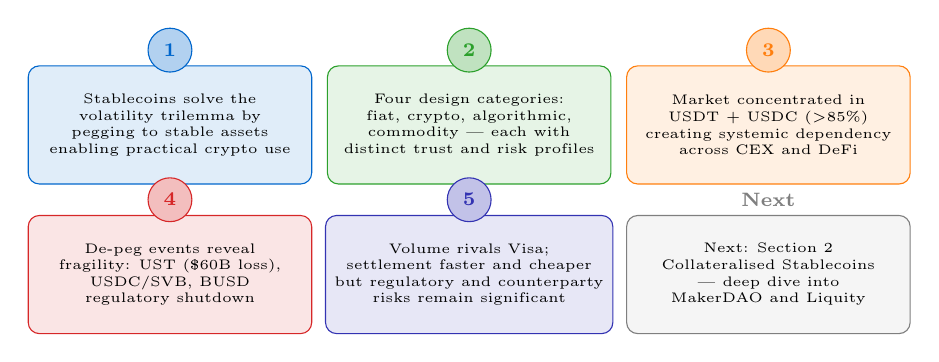
\begin{tikzpicture}
  \node[draw=mlblue, fill=mlblue!12, rounded corners=4pt, minimum width=3.6cm, minimum height=1.5cm, align=center, font=\tiny] (k1) at (1.9,3.2) {Stablecoins solve the\\volatility trilemma by\\pegging to stable assets\\enabling practical crypto use};
  \node[circle, draw=mlblue, fill=mlblue!30, minimum size=0.55cm, font=\scriptsize\bfseries, text=mlblue] at (1.9,4.15) {1};

  \node[draw=mlgreen, fill=mlgreen!12, rounded corners=4pt, minimum width=3.6cm, minimum height=1.5cm, align=center, font=\tiny] (k2) at (5.7,3.2) {Four design categories:\\fiat, crypto, algorithmic,\\commodity --- each with\\distinct trust and risk profiles};
  \node[circle, draw=mlgreen, fill=mlgreen!30, minimum size=0.55cm, font=\scriptsize\bfseries, text=mlgreen] at (5.7,4.15) {2};

  \node[draw=mlorange, fill=mlorange!12, rounded corners=4pt, minimum width=3.6cm, minimum height=1.5cm, align=center, font=\tiny] (k3) at (9.5,3.2) {Market concentrated in\\USDT + USDC ($>$85\%)\\creating systemic dependency\\across CEX and DeFi};
  \node[circle, draw=mlorange, fill=mlorange!30, minimum size=0.55cm, font=\scriptsize\bfseries, text=mlorange] at (9.5,4.15) {3};

  \node[draw=mlred, fill=mlred!12, rounded corners=4pt, minimum width=3.6cm, minimum height=1.5cm, align=center, font=\tiny] (k4) at (1.9,1.3) {De-peg events reveal\\fragility: UST (\$60B loss),\\USDC/SVB, BUSD\\regulatory shutdown};
  \node[circle, draw=mlred, fill=mlred!30, minimum size=0.55cm, font=\scriptsize\bfseries, text=mlred] at (1.9,2.25) {4};

  \node[draw=mlpurple, fill=mlpurple!12, rounded corners=4pt, minimum width=3.6cm, minimum height=1.5cm, align=center, font=\tiny] (k5) at (5.7,1.3) {Volume rivals Visa;\\settlement faster and cheaper\\but regulatory and counterparty\\risks remain significant};
  \node[circle, draw=mlpurple, fill=mlpurple!30, minimum size=0.55cm, font=\scriptsize\bfseries, text=mlpurple] at (5.7,2.25) {5};

  \node[draw=mlgray, fill=mlgray!8, rounded corners=4pt, minimum width=3.6cm, minimum height=1.5cm, align=center, font=\tiny] (k6) at (9.5,1.3) {Next: Section 2\\Collateralised Stablecoins\\--- deep dive into\\MakerDAO and Liquity};
  \node[font=\scriptsize\bfseries, text=mlgray] at (9.5,2.25) {Next};
\end{tikzpicture}
\bottomnote{Section 1 complete | 5 key takeaways | Proceed to Section 2: Collateralised Stablecoins for technical deep dive into CDP mechanisms}
\end{frame}

%% ============================================================
%% SECTION 2: COLLATERALIZED STABLECOINS
%% ============================================================
\section{Collateralized Stablecoins}

% Frame 15: Section 2 Divider
\begin{frame}{Section 2: Collateralized Stablecoins}
\begin{beamercolorbox}[sep=12pt,center,rounded=true,shadow=true]{palette quaternary}
  {\Large\bfseries Section 2: Collateralized Stablecoins}\\[4pt]
  {\normalsize Fiat-backed and crypto-backed approaches to maintaining price stability}
\end{beamercolorbox}

\vspace{4mm}
\begin{columns}[T]
\column{0.55\textwidth}
\begin{block}{What You Will Learn}
\begin{itemize}\setlength{\itemsep}{2pt}
  \item How fiat-backed stablecoins mint and redeem tokens
  \item USDT and USDC: architecture, reserves, and controversies
  \item Crypto-backed designs and over-collateralisation rationale
  \item MakerDAO / DAI: vaults, liquidation, multi-collateral
  \item Commodity-backed stablecoins (PAXG, XAUT)
\end{itemize}
\end{block}
\column{0.45\textwidth}
\begin{block}{Frames in This Section}
\begin{itemize}\setlength{\itemsep}{2pt}
  \item Frame 16: Fiat-Backed: How They Work
  \item Frame 17: USDT Deep Dive
  \item Frame 18: USDC Deep Dive
  \item Frame 19: Reserve Composition (Code)
  \item Frame 20: Crypto-Backed Overview
  \item Frame 21: MakerDAO and DAI
  \item Frame 22: Over-Collateralisation
  \item Frame 23: Liquidation Process
  \item Frame 24: Multi-Collateral DAI
  \item Frame 25: Commodity-Backed
  \item Frame 26: Section Summary
\end{itemize}
\end{block}
\end{columns}
\bottomnote{Section 2 of 5 | Frames 15--26 | Fiat-backed and crypto-backed stablecoin mechanisms in depth}
\end{frame}

% Frame 16: Fiat-Backed Stablecoins: How They Work
\begin{frame}{Fiat-Backed Stablecoins: How They Work}
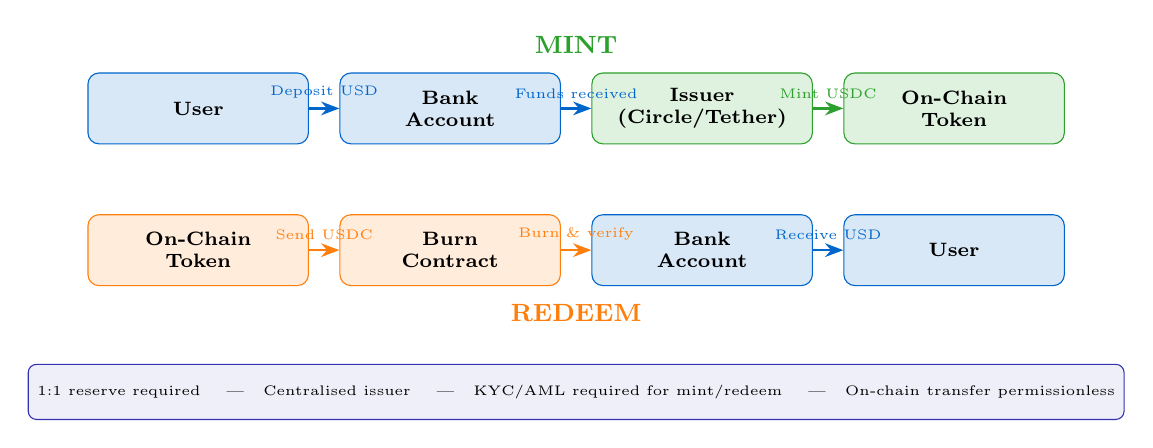
\begin{tikzpicture}
  %% --- MINT FLOW (top row) ---
  \node[draw=mlblue, fill=mlblue!15, rounded corners=4pt, minimum width=2.8cm, minimum height=0.9cm, align=center, font=\scriptsize\bfseries]    (user1)   at (0.0,4.2)  {User};
  \node[draw=mlblue, fill=mlblue!15, rounded corners=4pt, minimum width=2.8cm, minimum height=0.9cm, align=center, font=\scriptsize\bfseries]    (bank)    at (3.2,4.2)  {Bank\\Account};
  \node[draw=mlgreen, fill=mlgreen!15, rounded corners=4pt, minimum width=2.8cm, minimum height=0.9cm, align=center, font=\scriptsize\bfseries]   (issuer)  at (6.4,4.2)  {Issuer\\(Circle/Tether)};
  \node[draw=mlgreen, fill=mlgreen!15, rounded corners=4pt, minimum width=2.8cm, minimum height=0.9cm, align=center, font=\scriptsize\bfseries]   (chain)   at (9.6,4.2)  {On-Chain\\Token};

  \draw[-{Stealth}, thick, mlblue]  (user1.east)  -- (bank.west)   node[midway,above,font=\tiny,text=mlblue]  {Deposit USD};
  \draw[-{Stealth}, thick, mlblue]  (bank.east)   -- (issuer.west)  node[midway,above,font=\tiny,text=mlblue]  {Funds received};
  \draw[-{Stealth}, thick, mlgreen] (issuer.east) -- (chain.west)   node[midway,above,font=\tiny,text=mlgreen] {Mint USDC};

  %% --- REDEEM FLOW (bottom row) ---
  \node[draw=mlblue, fill=mlblue!15, rounded corners=4pt, minimum width=2.8cm, minimum height=0.9cm, align=center, font=\scriptsize\bfseries]    (user2)   at (9.6,2.4)  {User};
  \node[draw=mlblue, fill=mlblue!15, rounded corners=4pt, minimum width=2.8cm, minimum height=0.9cm, align=center, font=\scriptsize\bfseries]    (bank2)   at (6.4,2.4)  {Bank\\Account};
  \node[draw=mlorange, fill=mlorange!15, rounded corners=4pt, minimum width=2.8cm, minimum height=0.9cm, align=center, font=\scriptsize\bfseries]  (burn)    at (3.2,2.4)  {Burn\\Contract};
  \node[draw=mlorange, fill=mlorange!15, rounded corners=4pt, minimum width=2.8cm, minimum height=0.9cm, align=center, font=\scriptsize\bfseries]  (chain2)  at (0.0,2.4)  {On-Chain\\Token};

  \draw[-{Stealth}, thick, mlorange] (chain2.east) -- (burn.west)  node[midway,above,font=\tiny,text=mlorange] {Send USDC};
  \draw[-{Stealth}, thick, mlorange] (burn.east)   -- (bank2.west)  node[midway,above,font=\tiny,text=mlorange] {Burn \& verify};
  \draw[-{Stealth}, thick, mlblue]   (bank2.east)  -- (user2.west)  node[midway,above,font=\tiny,text=mlblue]   {Receive USD};

  %% --- LABELS ---
  \node[font=\small\bfseries, text=mlgreen] at (4.8,5.0) {MINT};
  \node[font=\small\bfseries, text=mlorange] at (4.8,1.6) {REDEEM};

  %% --- KEY PROPERTIES ---
  \node[draw=mlpurple, fill=mlpurple!8, rounded corners=3pt, minimum width=11.8cm, minimum height=0.7cm, align=center, font=\tiny] at (4.8,0.6)
    {1:1 reserve required \quad|\quad Centralised issuer \quad|\quad KYC/AML required for mint/redeem \quad|\quad On-chain transfer permissionless};
\end{tikzpicture}
\bottomnote{Fiat-backed stablecoins hold USD (or equivalents) in custody | Mint/redeem typically requires \$100k+ minimums | Secondary market provides retail access}
\end{frame}

% Frame 17: USDT (Tether) Deep Dive
\begin{frame}{USDT (Tether) Deep Dive}
\begin{columns}[T]
\column{0.48\textwidth}
\begin{block}{Key Facts}
\begin{itemize}\setlength{\itemsep}{2pt}
  \item \textbf{Launch:} 2014 (originally ``Realcoin'')
  \item \textbf{Issuer:} Tether Limited (British Virgin Islands)
  \item \textbf{Supply:} \$83B+ (largest stablecoin, 2023)
  \item \textbf{Chains:} Ethereum, Tron, Solana, BSC, Polygon
  \item \textbf{Tron share:} $\approx$50\% of USDT volume
  \item \textbf{Reserve attestations:} Quarterly (not full audits)
\end{itemize}
\end{block}
\vspace{2mm}
\begin{alertblock}{Controversy}
\scriptsize 2019 NYAG investigation: Tether used reserves to cover \$850M Bitfinex shortfall. Settled for \$18.5M. Raised questions about full reserve backing.
\end{alertblock}
\column{0.52\textwidth}
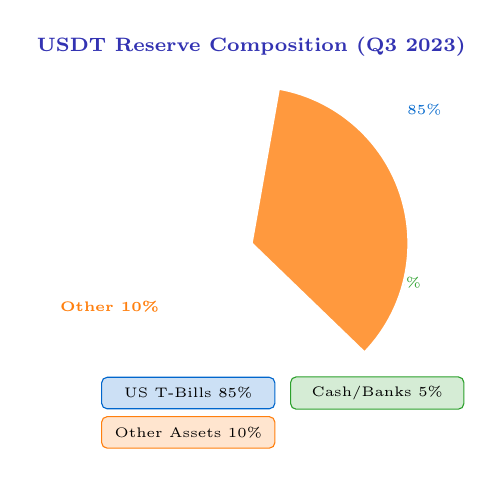
\begin{tikzpicture}[
  slice/.style={draw=white, line width=1pt}
]
  \node[font=\scriptsize\bfseries, text=mlpurple] at (2.8,5.3) {USDT Reserve Composition (Q3 2023)};
  %% US Treasuries ~85%
  \filldraw[fill=mlblue!80, slice] (2.8,2.8) -- ++(80:2.0) arc(80:-26:2.0) -- cycle;
  \node[font=\tiny\bfseries, text=white] at (3.4,3.6) {T-Bills};
  \node[font=\tiny, text=mlblue] at (5.0,4.5) {85\%};
  %% Cash ~5%
  \filldraw[fill=mlgreen!70, slice] (2.8,2.8) -- ++(-26:2.0) arc(-26:-44:2.0) -- cycle;
  \node[font=\tiny, text=mlgreen] at (4.5,2.3) {Cash 5\%};
  %% Other ~10%
  \filldraw[fill=mlorange!80, slice] (2.8,2.8) -- ++(-44:2.0) arc(-44:80:2.0) -- cycle;
  \node[font=\tiny\bfseries, text=mlorange] at (1.0,2.0) {Other 10\%};
  \node[font=\tiny, text=mlgray] at (2.8,2.8) {};
  %% Legend
  \node[draw=mlblue,   fill=mlblue!20,   rounded corners=2pt, minimum width=2.2cm, minimum height=0.4cm, font=\tiny, align=center] at (2.0,0.9) {US T-Bills 85\%};
  \node[draw=mlgreen,  fill=mlgreen!20,  rounded corners=2pt, minimum width=2.2cm, minimum height=0.4cm, font=\tiny, align=center] at (4.4,0.9) {Cash/Banks 5\%};
  \node[draw=mlorange, fill=mlorange!20, rounded corners=2pt, minimum width=2.2cm, minimum height=0.4cm, font=\tiny, align=center] at (2.0,0.4) {Other Assets 10\%};
\end{tikzpicture}
\end{columns}
\bottomnote{USDT dominates stablecoin volume | Tether Q3 2023 attestation: BDO Italia | Full audit never published | Key systemic risk due to market size}
\end{frame}

% Frame 18: USDC (Circle) Deep Dive
\begin{frame}{USDC (Circle) Deep Dive}
\begin{columns}[T]
\column{0.48\textwidth}
\begin{block}{Key Facts}
\begin{itemize}\setlength{\itemsep}{2pt}
  \item \textbf{Launch:} 2018 (Circle + Coinbase consortium)
  \item \textbf{Issuer:} Circle Internet Financial (Boston, MA)
  \item \textbf{Supply:} \$25B+ (2023, down from \$56B peak)
  \item \textbf{Reserves:} 100\% cash + short-term US Treasuries
  \item \textbf{Attestations:} Monthly by Deloitte
  \item \textbf{Regulation:} NY BitLicense; EU MiCA compliant path
\end{itemize}
\end{block}
\vspace{2mm}
\begin{block}{Transparency Advantage}
\begin{itemize}\setlength{\itemsep}{1pt}
  \item Monthly reserve attestations (public)
  \item Segregated reserve account at regulated banks
  \item SVB incident (Mar 2023): \$3.3B exposed, brief de-peg to \$0.87
  \item Recovered within 48h after FDIC guarantee announcement
\end{itemize}
\end{block}
\column{0.52\textwidth}
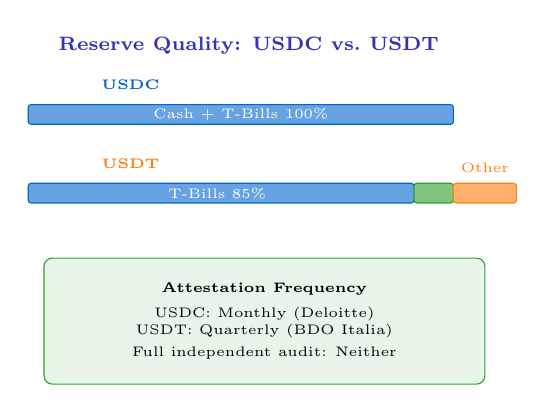
\begin{tikzpicture}
  \node[font=\scriptsize\bfseries, text=mlpurple] at (3.0,5.3) {Reserve Quality: USDC vs.\ USDT};
  %% USDC bar
  \node[font=\tiny\bfseries, text=mlblue] at (1.5,4.8) {USDC};
  \filldraw[draw=mlblue, fill=mlblue!60, rounded corners=1pt]   (0.2,4.3) rectangle (5.6,4.55);
  \node[font=\tiny, text=white] at (2.9,4.42) {Cash + T-Bills 100\%};
  %% USDT bar
  \node[font=\tiny\bfseries, text=mlorange] at (1.5,3.8) {USDT};
  \filldraw[draw=mlblue, fill=mlblue!60, rounded corners=1pt]   (0.2,3.3) rectangle (5.1,3.55);
  \node[font=\tiny, text=white] at (2.6,3.42) {T-Bills 85\%};
  \filldraw[draw=mlgreen, fill=mlgreen!60, rounded corners=1pt]  (5.1,3.3) rectangle (5.6,3.55);
  \filldraw[draw=mlorange, fill=mlorange!60, rounded corners=1pt] (5.6,3.3) rectangle (6.4,3.55);
  \node[font=\tiny, text=mlorange] at (6.0,3.75) {Other};
  %% Attestation frequency
  \node[draw=mlgreen, fill=mlgreen!10, rounded corners=3pt, minimum width=5.6cm, minimum height=1.6cm, align=center, font=\tiny] at (3.2,1.8)
    {\textbf{Attestation Frequency}\\[3pt]
     USDC: Monthly (Deloitte)\\
     USDT: Quarterly (BDO Italia)\\[2pt]
     Full independent audit: Neither};
\end{tikzpicture}
\end{columns}
\bottomnote{USDC lost market share after SVB (Mar 2023) and Binance halted BUSD (Feb 2023) | Circle files S-1 for IPO 2024 | MiCA compliance path established}
\end{frame}

% Frame 19: Reserve Composition Comparison (Code Frame)
\begin{frame}[fragile]{Reserve Composition: Smart Contract Interface}
\begin{columns}[T]
\column{0.50\textwidth}
\begin{lstlisting}[language=Solidity, caption={Stablecoin Interface}]
// SPDX-License-Identifier: MIT
pragma solidity ^0.8.0;

interface IStablecoin {
    function mint(address to, uint256 amount)
        external;
    function burn(address from, uint256 amount)
        external;
    function totalSupply()
        external view returns (uint256);
    function reserveBalance()
        external view returns (uint256);
    function collateralRatio()
        external view returns (uint256);
}
\end{lstlisting}
\column{0.50\textwidth}
\begin{block}{Interface Explanation}
\begin{itemize}\setlength{\itemsep}{3pt}
  \item \textbf{mint}: Creates new tokens when USD deposited; restricted to issuer
  \item \textbf{burn}: Destroys tokens on redemption; releases equivalent USD
  \item \textbf{totalSupply}: Circulating token count; must equal reserve for 1:1 peg
  \item \textbf{reserveBalance}: Off-chain verified reserve value in USD (18 decimals)
  \item \textbf{collateralRatio}: $\frac{\text{reserveBalance}}{\text{totalSupply}} \times 100$ --- should be $\geq 100$
\end{itemize}
\end{block}
\vspace{2mm}
\begin{alertblock}{Key Insight}
\scriptsize Fiat-backed issuers publish \texttt{totalSupply} on-chain but \texttt{reserveBalance} is off-chain attested. The gap between on-chain and off-chain is the core trust assumption.
\end{alertblock}
\end{columns}
\bottomnote{USDC contract: 0xA0b86991c6218b36c1d19D4a2e9Eb0cE3606eB48 (Ethereum) | Solidity interface pattern | Collateral ratio audit: off-chain attestation required}
\end{frame}

% Frame 20: Crypto-Backed Stablecoins: Overview
\begin{frame}{Crypto-Backed Stablecoins: Overview}
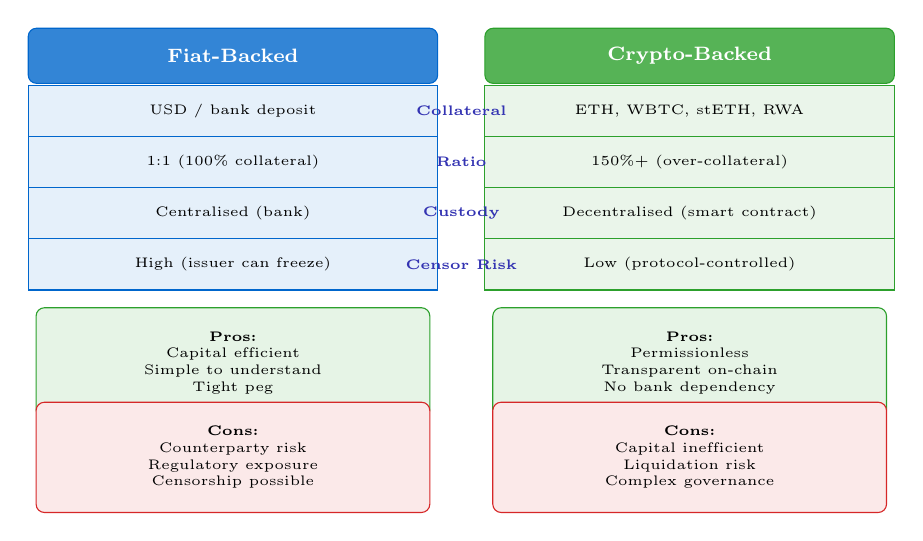
\begin{tikzpicture}[
  pro/.style={draw=mlgreen, fill=mlgreen!12, rounded corners=3pt, minimum width=5.0cm, minimum height=1.4cm, align=center, font=\tiny},
  con/.style={draw=mlred,   fill=mlred!10,   rounded corners=3pt, minimum width=5.0cm, minimum height=1.4cm, align=center, font=\tiny}
]
  %% Table header
  \node[draw=mlblue, fill=mlblue!80, rounded corners=3pt, minimum width=5.2cm, minimum height=0.7cm, align=center, font=\scriptsize\bfseries, text=white]   (h1) at (2.8,5.0) {Fiat-Backed};
  \node[draw=mlgreen, fill=mlgreen!80, rounded corners=3pt, minimum width=5.2cm, minimum height=0.7cm, align=center, font=\scriptsize\bfseries, text=white]  (h2) at (8.6,5.0) {Crypto-Backed};

  %% Row 1: Collateral
  \node[draw=mlblue, fill=mlblue!10, minimum width=5.2cm, minimum height=0.65cm, align=center, font=\tiny]  at (2.8,4.3) {USD / bank deposit};
  \node[draw=mlgreen, fill=mlgreen!10, minimum width=5.2cm, minimum height=0.65cm, align=center, font=\tiny] at (8.6,4.3) {ETH, WBTC, stETH, RWA};
  \node[font=\tiny\bfseries, text=mlpurple] at (5.7,4.3) {Collateral};

  %% Row 2: Ratio
  \node[draw=mlblue, fill=mlblue!10, minimum width=5.2cm, minimum height=0.65cm, align=center, font=\tiny]  at (2.8,3.65) {1:1 (100\% collateral)};
  \node[draw=mlgreen, fill=mlgreen!10, minimum width=5.2cm, minimum height=0.65cm, align=center, font=\tiny] at (8.6,3.65) {150\%+ (over-collateral)};
  \node[font=\tiny\bfseries, text=mlpurple] at (5.7,3.65) {Ratio};

  %% Row 3: Custody
  \node[draw=mlblue, fill=mlblue!10, minimum width=5.2cm, minimum height=0.65cm, align=center, font=\tiny]  at (2.8,3.0) {Centralised (bank)};
  \node[draw=mlgreen, fill=mlgreen!10, minimum width=5.2cm, minimum height=0.65cm, align=center, font=\tiny] at (8.6,3.0) {Decentralised (smart contract)};
  \node[font=\tiny\bfseries, text=mlpurple] at (5.7,3.0) {Custody};

  %% Row 4: Censor risk
  \node[draw=mlblue, fill=mlblue!10, minimum width=5.2cm, minimum height=0.65cm, align=center, font=\tiny]  at (2.8,2.35) {High (issuer can freeze)};
  \node[draw=mlgreen, fill=mlgreen!10, minimum width=5.2cm, minimum height=0.65cm, align=center, font=\tiny] at (8.6,2.35) {Low (protocol-controlled)};
  \node[font=\tiny\bfseries, text=mlpurple] at (5.7,2.35) {Censor Risk};

  %% Pros / Cons
  \node[pro] (p1) at (2.8,1.1) {\textbf{Pros:}\\Capital efficient\\Simple to understand\\Tight peg};
  \node[pro] (p2) at (8.6,1.1) {\textbf{Pros:}\\Permissionless\\Transparent on-chain\\No bank dependency};
  \node[con] (c1) at (2.8,-0.1) {\textbf{Cons:}\\Counterparty risk\\Regulatory exposure\\Censorship possible};
  \node[con] (c2) at (8.6,-0.1) {\textbf{Cons:}\\Capital inefficient\\Liquidation risk\\Complex governance};
\end{tikzpicture}
\bottomnote{Crypto-backed stablecoins: DAI (\$5B+), sUSD, LUSD | Over-collateralisation absorbs crypto price volatility | CDP = Collateralised Debt Position}
\end{frame}

% Frame 21: MakerDAO and DAI
\begin{frame}{MakerDAO and DAI}
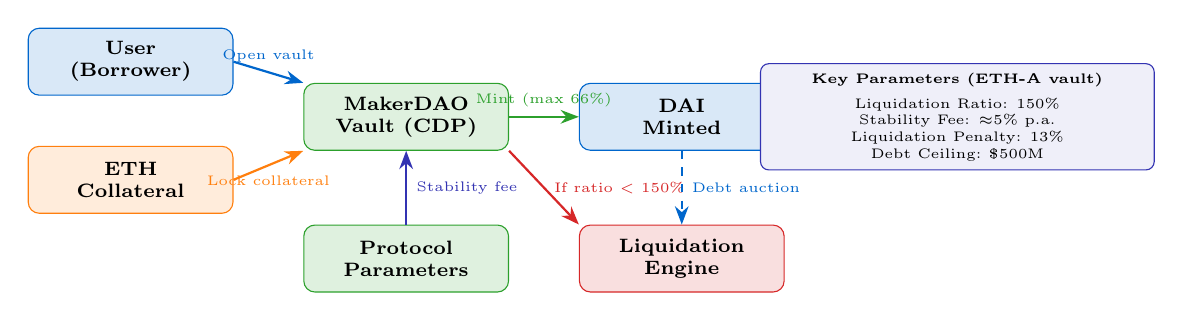
\begin{tikzpicture}
  %% Deposit
  \node[draw=mlblue, fill=mlblue!15, rounded corners=4pt, minimum width=2.6cm, minimum height=0.85cm, align=center, font=\scriptsize\bfseries]  (user)   at (0.0,3.5) {User\\(Borrower)};
  \node[draw=mlorange, fill=mlorange!15, rounded corners=4pt, minimum width=2.6cm, minimum height=0.85cm, align=center, font=\scriptsize\bfseries] (eth)   at (0.0,2.0) {ETH\\Collateral};
  \node[draw=mlgreen, fill=mlgreen!15, rounded corners=4pt, minimum width=2.6cm, minimum height=0.85cm, align=center, font=\scriptsize\bfseries]  (vault) at (3.5,2.8) {MakerDAO\\Vault (CDP)};
  \node[draw=mlblue, fill=mlblue!15, rounded corners=4pt, minimum width=2.6cm, minimum height=0.85cm, align=center, font=\scriptsize\bfseries]   (dai)   at (7.0,2.8) {DAI\\Minted};
  \node[draw=mlgreen, fill=mlgreen!15, rounded corners=4pt, minimum width=2.6cm, minimum height=0.85cm, align=center, font=\scriptsize\bfseries]  (proto) at (3.5,1.0) {Protocol\\Parameters};
  \node[draw=mlred, fill=mlred!15, rounded corners=4pt, minimum width=2.6cm, minimum height=0.85cm, align=center, font=\scriptsize\bfseries]    (liq)   at (7.0,1.0) {Liquidation\\Engine};

  \draw[-{Stealth}, thick, mlblue]   (user.east)  -- (vault.north west) node[midway,above,font=\tiny,text=mlblue]   {Open vault};
  \draw[-{Stealth}, thick, mlorange] (eth.east)   -- (vault.south west) node[midway,below,font=\tiny,text=mlorange]  {Lock collateral};
  \draw[-{Stealth}, thick, mlgreen]  (vault.east) -- (dai.west)          node[midway,above,font=\tiny,text=mlgreen]   {Mint (max 66\%)};
  \draw[-{Stealth}, thick, mlpurple] (proto.north) -- (vault.south)      node[midway,right,font=\tiny,text=mlpurple] {Stability fee};
  \draw[-{Stealth}, thick, mlred]    (vault.south east) -- (liq.north west) node[midway,right,font=\tiny,text=mlred]{If ratio $<$ 150\%};
  \draw[-{Stealth}, thick, mlblue, dashed] (dai.south) -- (liq.north)     node[midway,right,font=\tiny,text=mlblue]  {Debt auction};

  %% Key parameters box
  \node[draw=mlpurple, fill=mlpurple!8, rounded corners=3pt, minimum width=5.0cm, minimum height=1.2cm, align=center, font=\tiny] at (10.5,2.8)
    {\textbf{Key Parameters (ETH-A vault)}\\[3pt]
     Liquidation Ratio: 150\%\\
     Stability Fee: $\approx$5\% p.a.\\
     Liquidation Penalty: 13\%\\
     Debt Ceiling: \$500M};
\end{tikzpicture}
\bottomnote{MakerDAO launched 2017 | DAI peg maintained via stability fee adjustments and PSM | MKR holders govern protocol parameters | \$8B+ TVL peak 2022}
\end{frame}

% Frame 22: Over-Collateralisation Mechanics
\begin{frame}{Over-Collateralisation Mechanics}
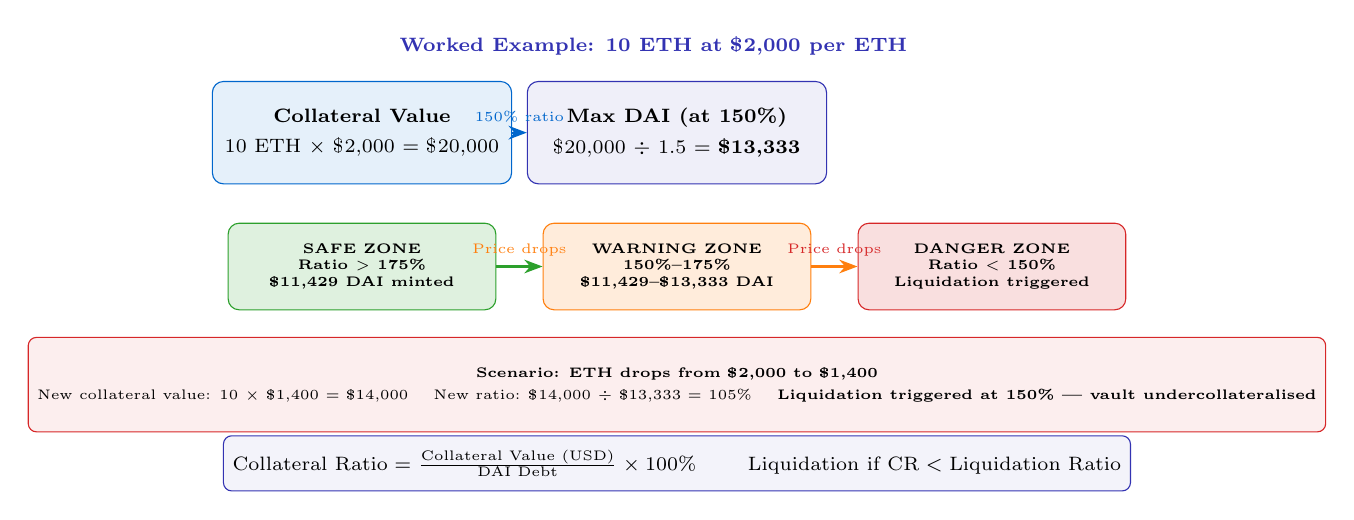
\begin{tikzpicture}
  %% Title annotation
  \node[font=\scriptsize\bfseries, text=mlpurple] at (5.5,5.6) {Worked Example: 10 ETH at \$2{,}000 per ETH};

  %% Input box
  \node[draw=mlblue, fill=mlblue!10, rounded corners=4pt, minimum width=3.8cm, minimum height=1.3cm, align=center, font=\scriptsize] (input) at (1.8,4.5)
    {\textbf{Collateral Value}\\[3pt]10 ETH $\times$ \$2{,}000 = \$20{,}000};

  %% Ratio calculation
  \node[draw=mlpurple, fill=mlpurple!8, rounded corners=4pt, minimum width=3.8cm, minimum height=1.3cm, align=center, font=\scriptsize] (ratio) at (5.8,4.5)
    {\textbf{Max DAI (at 150\%)}\\[3pt]\$20{,}000 $\div$ 1.5 = \textbf{\$13{,}333}};

  \draw[-{Stealth}, thick, mlblue] (input.east) -- (ratio.west) node[midway,above,font=\tiny,text=mlblue] {150\% ratio};

  %% Zone table
  \node[draw=mlgreen, fill=mlgreen!15, rounded corners=4pt, minimum width=3.4cm, minimum height=1.1cm, align=center, font=\tiny\bfseries]  (safe) at (1.8,2.8)    {SAFE ZONE\\Ratio $>$ 175\%\\\$11{,}429 DAI minted};
  \node[draw=mlorange, fill=mlorange!15, rounded corners=4pt, minimum width=3.4cm, minimum height=1.1cm, align=center, font=\tiny\bfseries] (warn) at (5.8,2.8)    {WARNING ZONE\\150\%--175\%\\\$11{,}429--\$13{,}333 DAI};
  \node[draw=mlred, fill=mlred!15, rounded corners=4pt, minimum width=3.4cm, minimum height=1.1cm, align=center, font=\tiny\bfseries]    (dang) at (9.8,2.8)    {DANGER ZONE\\Ratio $<$ 150\%\\Liquidation triggered};

  \draw[-{Stealth}, thick, mlgreen]  (safe.east)  -- (warn.west)  node[midway,above,font=\tiny,text=mlorange] {Price drops};
  \draw[-{Stealth}, thick, mlorange] (warn.east)  -- (dang.west)  node[midway,above,font=\tiny,text=mlred]    {Price drops};

  %% Price drop scenario
  \node[draw=mlred, fill=mlred!8, rounded corners=3pt, minimum width=10.8cm, minimum height=1.2cm, align=center, font=\tiny] at (5.8,1.3)
    {\textbf{Scenario: ETH drops from \$2{,}000 to \$1{,}400}\\[2pt]
     New collateral value: 10 $\times$ \$1{,}400 = \$14{,}000 \quad
     New ratio: \$14{,}000 $\div$ \$13{,}333 = 105\% \quad
     \textbf{Liquidation triggered at 150\% --- vault undercollateralised}};

  %% Formula
  \node[draw=mlpurple, fill=mlpurple!6, rounded corners=3pt, minimum width=10.8cm, minimum height=0.7cm, align=center, font=\scriptsize] at (5.8,0.3)
    {$\text{Collateral Ratio} = \frac{\text{Collateral Value (USD)}}{\text{DAI Debt}} \times 100\%$
     \qquad Liquidation if $\text{CR} < \text{Liquidation Ratio}$};
\end{tikzpicture}
\bottomnote{Over-collateralisation buffers against crypto volatility | ETH 30-day volatility $\approx$60\% annualised | 150\% ratio provides $\approx$33\% price drop buffer before liquidation}
\end{frame}

% Frame 23: Liquidation Process
\begin{frame}{Liquidation Process}
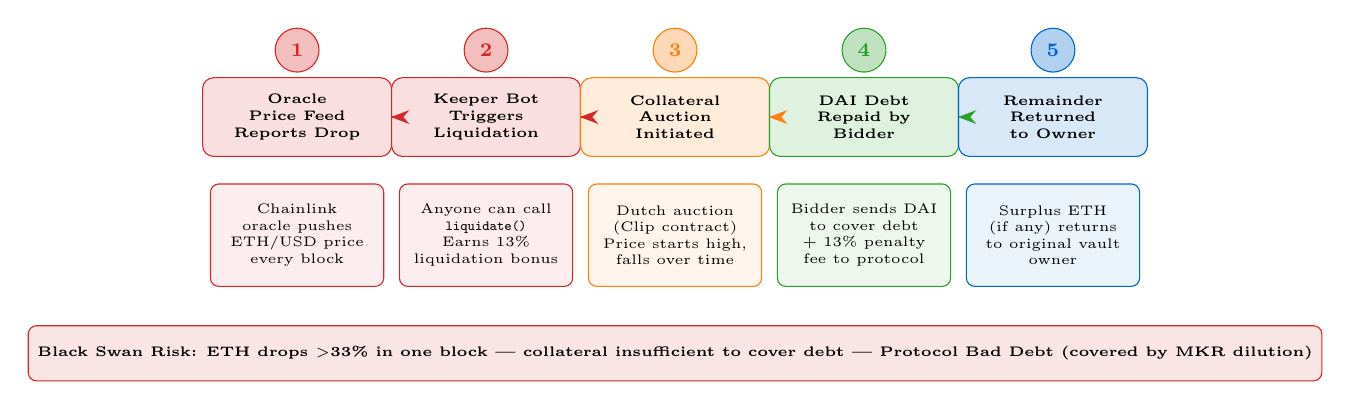
\begin{tikzpicture}
  %% Step boxes
  \node[draw=mlred, fill=mlred!15, rounded corners=4pt, minimum width=2.4cm, minimum height=1.0cm, align=center, font=\tiny\bfseries]     (s1) at (0.8,3.8)  {Oracle\\Price Feed\\Reports Drop};
  \node[draw=mlred, fill=mlred!15, rounded corners=4pt, minimum width=2.4cm, minimum height=1.0cm, align=center, font=\tiny\bfseries]     (s2) at (3.2,3.8)  {Keeper Bot\\Triggers\\Liquidation};
  \node[draw=mlorange, fill=mlorange!15, rounded corners=4pt, minimum width=2.4cm, minimum height=1.0cm, align=center, font=\tiny\bfseries]  (s3) at (5.6,3.8)  {Collateral\\Auction\\Initiated};
  \node[draw=mlgreen, fill=mlgreen!15, rounded corners=4pt, minimum width=2.4cm, minimum height=1.0cm, align=center, font=\tiny\bfseries]   (s4) at (8.0,3.8)  {DAI Debt\\Repaid by\\Bidder};
  \node[draw=mlblue, fill=mlblue!15, rounded corners=4pt, minimum width=2.4cm, minimum height=1.0cm, align=center, font=\tiny\bfseries]    (s5) at (10.4,3.8) {Remainder\\Returned\\to Owner};

  %% Arrows
  \draw[-{Stealth}, thick, mlred]    (s1.east) -- (s2.west);
  \draw[-{Stealth}, thick, mlred]    (s2.east) -- (s3.west);
  \draw[-{Stealth}, thick, mlorange] (s3.east) -- (s4.west);
  \draw[-{Stealth}, thick, mlgreen]  (s4.east) -- (s5.west);

  %% Step numbers
  \node[circle, draw=mlred, fill=mlred!30, minimum size=0.5cm, font=\scriptsize\bfseries, text=mlred]    at (0.8,4.65)  {1};
  \node[circle, draw=mlred, fill=mlred!30, minimum size=0.5cm, font=\scriptsize\bfseries, text=mlred]    at (3.2,4.65)  {2};
  \node[circle, draw=mlorange, fill=mlorange!30, minimum size=0.5cm, font=\scriptsize\bfseries, text=mlorange] at (5.6,4.65)  {3};
  \node[circle, draw=mlgreen, fill=mlgreen!30, minimum size=0.5cm, font=\scriptsize\bfseries, text=mlgreen]  at (8.0,4.65)  {4};
  \node[circle, draw=mlblue, fill=mlblue!30, minimum size=0.5cm, font=\scriptsize\bfseries, text=mlblue]   at (10.4,4.65) {5};

  %% Details boxes
  \node[draw=mlred, fill=mlred!8, rounded corners=3pt, minimum width=2.2cm, minimum height=1.3cm, align=center, font=\tiny] at (0.8,2.3)
    {Chainlink\\oracle pushes\\ETH/USD price\\every block};
  \node[draw=mlred, fill=mlred!8, rounded corners=3pt, minimum width=2.2cm, minimum height=1.3cm, align=center, font=\tiny] at (3.2,2.3)
    {Anyone can call\\\texttt{liquidate()}\\Earns 13\%\\liquidation bonus};
  \node[draw=mlorange, fill=mlorange!8, rounded corners=3pt, minimum width=2.2cm, minimum height=1.3cm, align=center, font=\tiny] at (5.6,2.3)
    {Dutch auction\\(Clip contract)\\Price starts high,\\falls over time};
  \node[draw=mlgreen, fill=mlgreen!8, rounded corners=3pt, minimum width=2.2cm, minimum height=1.3cm, align=center, font=\tiny] at (8.0,2.3)
    {Bidder sends DAI\\to cover debt\\+ 13\% penalty\\fee to protocol};
  \node[draw=mlblue, fill=mlblue!8, rounded corners=3pt, minimum width=2.2cm, minimum height=1.3cm, align=center, font=\tiny] at (10.4,2.3)
    {Surplus ETH\\(if any) returns\\to original vault\\owner};

  %% Warning
  \node[draw=mlred, fill=mlred!12, rounded corners=3pt, minimum width=11.0cm, minimum height=0.7cm, align=center, font=\tiny\bfseries] at (5.6,0.8)
    {Black Swan Risk: ETH drops $>$33\% in one block --- collateral insufficient to cover debt --- Protocol Bad Debt (covered by MKR dilution)};
\end{tikzpicture}
\bottomnote{MakerDAO liquidations: \$240M+ in March 2020 ``Black Thursday'' | Keeper network monitors $\approx$50{,}000 vaults | Clip auction system introduced in MCD upgrade 2021}
\end{frame}

% Frame 24: Multi-Collateral DAI
\begin{frame}{Multi-Collateral DAI}
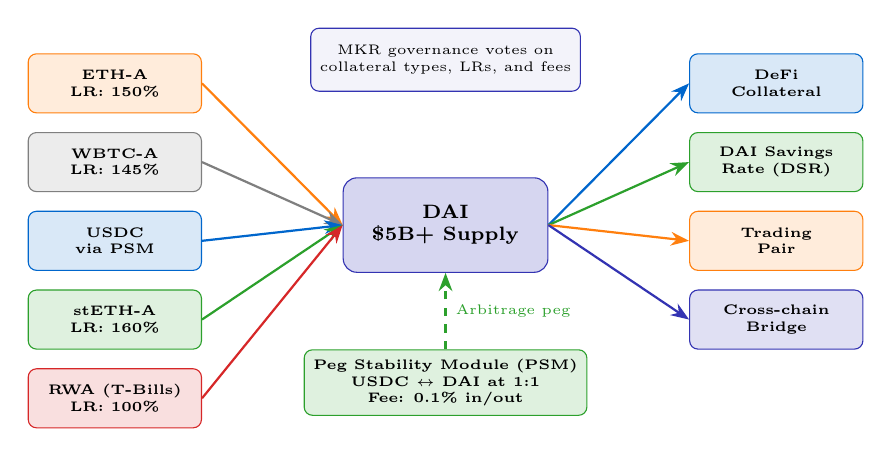
\begin{tikzpicture}[
  dai/.style={draw=mlpurple, fill=mlpurple!20, rounded corners=5pt, minimum width=2.6cm, minimum height=1.2cm, align=center, font=\scriptsize\bfseries},
  psm/.style={draw=mlgreen, fill=mlgreen!15, rounded corners=3pt, minimum width=3.0cm, minimum height=0.75cm, align=center, font=\tiny\bfseries}
]
  %% Central DAI node
  \node[dai] (dai) at (6.0,3.2) {DAI\\\$5B+ Supply};

  %% Collateral inputs (left side)
  \node[draw=mlorange, fill=mlorange!15, rounded corners=3pt, minimum width=2.2cm, minimum height=0.75cm, align=center, font=\tiny\bfseries] (eth)   at (1.8,5.0) {ETH-A\\LR: 150\%};
  \node[draw=mlgray, fill=mlgray!15, rounded corners=3pt, minimum width=2.2cm, minimum height=0.75cm, align=center, font=\tiny\bfseries]   (wbtc)  at (1.8,4.0) {WBTC-A\\LR: 145\%};
  \node[draw=mlblue, fill=mlblue!15, rounded corners=3pt, minimum width=2.2cm, minimum height=0.75cm, align=center, font=\tiny\bfseries]   (usdc)  at (1.8,3.0) {USDC\\via PSM};
  \node[draw=mlgreen, fill=mlgreen!15, rounded corners=3pt, minimum width=2.2cm, minimum height=0.75cm, align=center, font=\tiny\bfseries]  (stetH) at (1.8,2.0) {stETH-A\\LR: 160\%};
  \node[draw=mlred, fill=mlred!15, rounded corners=3pt, minimum width=2.2cm, minimum height=0.75cm, align=center, font=\tiny\bfseries]    (rwa)   at (1.8,1.0) {RWA (T-Bills)\\LR: 100\%};

  \draw[-{Stealth}, thick, mlorange] (eth.east)   -- (dai.west);
  \draw[-{Stealth}, thick, mlgray]   (wbtc.east)  -- (dai.west);
  \draw[-{Stealth}, thick, mlblue]   (usdc.east)  -- (dai.west);
  \draw[-{Stealth}, thick, mlgreen]  (stetH.east) -- (dai.west);
  \draw[-{Stealth}, thick, mlred]    (rwa.east)   -- (dai.west);

  %% PSM box
  \node[psm] (psm) at (6.0,1.2)
    {Peg Stability Module (PSM)\\USDC $\leftrightarrow$ DAI at 1:1\\Fee: 0.1\% in/out};
  \draw[-{Stealth}, thick, mlgreen, dashed] (psm.north) -- (dai.south) node[midway,right,font=\tiny,text=mlgreen] {Arbitrage peg};

  %% Output: use cases
  \node[draw=mlblue, fill=mlblue!15, rounded corners=3pt, minimum width=2.2cm, minimum height=0.75cm, align=center, font=\tiny\bfseries]   (defi)  at (10.2,5.0) {DeFi\\Collateral};
  \node[draw=mlgreen, fill=mlgreen!15, rounded corners=3pt, minimum width=2.2cm, minimum height=0.75cm, align=center, font=\tiny\bfseries]  (save)  at (10.2,4.0) {DAI Savings\\Rate (DSR)};
  \node[draw=mlorange, fill=mlorange!15, rounded corners=3pt, minimum width=2.2cm, minimum height=0.75cm, align=center, font=\tiny\bfseries] (trade) at (10.2,3.0) {Trading\\Pair};
  \node[draw=mlpurple, fill=mlpurple!15, rounded corners=3pt, minimum width=2.2cm, minimum height=0.75cm, align=center, font=\tiny\bfseries] (brdg)  at (10.2,2.0) {Cross-chain\\Bridge};

  \draw[-{Stealth}, thick, mlblue]   (dai.east) -- (defi.west);
  \draw[-{Stealth}, thick, mlgreen]  (dai.east) -- (save.west);
  \draw[-{Stealth}, thick, mlorange] (dai.east) -- (trade.west);
  \draw[-{Stealth}, thick, mlpurple] (dai.east) -- (brdg.west);

  %% Governance note
  \node[draw=mlpurple, fill=mlpurple!6, rounded corners=3pt, minimum width=3.2cm, minimum height=0.8cm, align=center, font=\tiny] at (6.0,5.3)
    {MKR governance votes on\\collateral types, LRs, and fees};
\end{tikzpicture}
\bottomnote{MCD launched Nov 2019 | PSM introduced 2020 for USDC 1:1 swap | RWA (real-world assets) added 2022 -- Monetalis Clydesdale holds US Treasuries | DSR: 5\% (2023)}
\end{frame}

% Frame 25: Commodity-Backed Stablecoins
\begin{frame}{Commodity-Backed Stablecoins}
\begin{columns}[T]
\column{0.50\textwidth}
\begin{block}{PAX Gold (PAXG)}
\begin{itemize}\setlength{\itemsep}{2pt}
  \item \textbf{Issuer:} Paxos Trust Company (NYDFS regulated)
  \item \textbf{Backing:} 1 PAXG = 1 troy ounce of LBMA gold
  \item \textbf{Storage:} Brinks vaults, London
  \item \textbf{Redemption:} Physical gold or cash (min.\ 430 oz)
  \item \textbf{Supply:} $\approx$250{,}000 oz (\$500M+ at \$2{,}000/oz)
  \item \textbf{Attestation:} Monthly by WithumSmith+Brown
\end{itemize}
\end{block}
\vspace{2mm}
\begin{block}{Tether Gold (XAUT)}
\begin{itemize}\setlength{\itemsep}{2pt}
  \item \textbf{Issuer:} Tether (British Virgin Islands)
  \item \textbf{Backing:} 1 XAUT = 1 troy ounce of fine gold
  \item \textbf{Storage:} Swiss vaults (undisclosed locations)
  \item \textbf{Attestation:} Quarterly (same as USDT)
  \item \textbf{Supply:} $\approx$246{,}000 oz
\end{itemize}
\end{block}
\column{0.50\textwidth}
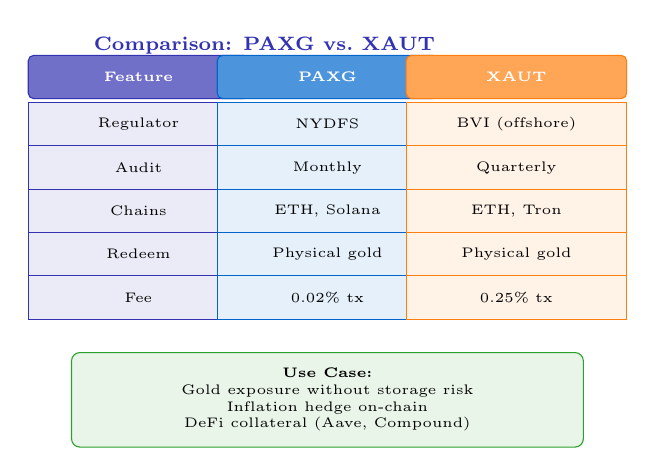
\begin{tikzpicture}
  \node[font=\scriptsize\bfseries, text=mlpurple] at (3.2,5.4) {Comparison: PAXG vs.\ XAUT};

  \node[draw=mlpurple, fill=mlpurple!70, minimum width=2.8cm, minimum height=0.55cm, align=center, font=\tiny\bfseries, text=white, rounded corners=2pt] at (1.6,5.0) {Feature};
  \node[draw=mlblue, fill=mlblue!70, minimum width=2.8cm, minimum height=0.55cm, align=center, font=\tiny\bfseries, text=white, rounded corners=2pt]   at (4.0,5.0) {PAXG};
  \node[draw=mlorange, fill=mlorange!70, minimum width=2.8cm, minimum height=0.55cm, align=center, font=\tiny\bfseries, text=white, rounded corners=2pt] at (6.4,5.0) {XAUT};

  \node[draw=mlpurple, fill=mlpurple!10, minimum width=2.8cm, minimum height=0.55cm, align=center, font=\tiny] at (1.6,4.4) {Regulator};
  \node[draw=mlblue, fill=mlblue!10, minimum width=2.8cm, minimum height=0.55cm, align=center, font=\tiny]   at (4.0,4.4) {NYDFS};
  \node[draw=mlorange, fill=mlorange!10, minimum width=2.8cm, minimum height=0.55cm, align=center, font=\tiny] at (6.4,4.4) {BVI (offshore)};

  \node[draw=mlpurple, fill=mlpurple!10, minimum width=2.8cm, minimum height=0.55cm, align=center, font=\tiny] at (1.6,3.85) {Audit};
  \node[draw=mlblue, fill=mlblue!10, minimum width=2.8cm, minimum height=0.55cm, align=center, font=\tiny]   at (4.0,3.85) {Monthly};
  \node[draw=mlorange, fill=mlorange!10, minimum width=2.8cm, minimum height=0.55cm, align=center, font=\tiny] at (6.4,3.85) {Quarterly};

  \node[draw=mlpurple, fill=mlpurple!10, minimum width=2.8cm, minimum height=0.55cm, align=center, font=\tiny] at (1.6,3.3) {Chains};
  \node[draw=mlblue, fill=mlblue!10, minimum width=2.8cm, minimum height=0.55cm, align=center, font=\tiny]   at (4.0,3.3) {ETH, Solana};
  \node[draw=mlorange, fill=mlorange!10, minimum width=2.8cm, minimum height=0.55cm, align=center, font=\tiny] at (6.4,3.3) {ETH, Tron};

  \node[draw=mlpurple, fill=mlpurple!10, minimum width=2.8cm, minimum height=0.55cm, align=center, font=\tiny] at (1.6,2.75) {Redeem};
  \node[draw=mlblue, fill=mlblue!10, minimum width=2.8cm, minimum height=0.55cm, align=center, font=\tiny]   at (4.0,2.75) {Physical gold};
  \node[draw=mlorange, fill=mlorange!10, minimum width=2.8cm, minimum height=0.55cm, align=center, font=\tiny] at (6.4,2.75) {Physical gold};

  \node[draw=mlpurple, fill=mlpurple!10, minimum width=2.8cm, minimum height=0.55cm, align=center, font=\tiny] at (1.6,2.2) {Fee};
  \node[draw=mlblue, fill=mlblue!10, minimum width=2.8cm, minimum height=0.55cm, align=center, font=\tiny]   at (4.0,2.2) {0.02\% tx};
  \node[draw=mlorange, fill=mlorange!10, minimum width=2.8cm, minimum height=0.55cm, align=center, font=\tiny] at (6.4,2.2) {0.25\% tx};

  \node[draw=mlgreen, fill=mlgreen!10, rounded corners=3pt, minimum width=6.5cm, minimum height=1.2cm, align=center, font=\tiny] at (4.0,0.9)
    {\textbf{Use Case:}\\Gold exposure without storage risk\\Inflation hedge on-chain\\DeFi collateral (Aave, Compound)};
\end{tikzpicture}
\end{columns}
\bottomnote{Gold-backed stablecoins: \$1B+ combined market cap | PAXG price tracks LBMA spot gold | Volatility $\approx$15\% annualised (vs.\ 70\%+ for BTC) | Not ideal for DeFi collateral due to price moves}
\end{frame}

% Frame 26: Section 2 Summary
\begin{frame}{Section 2 Summary}
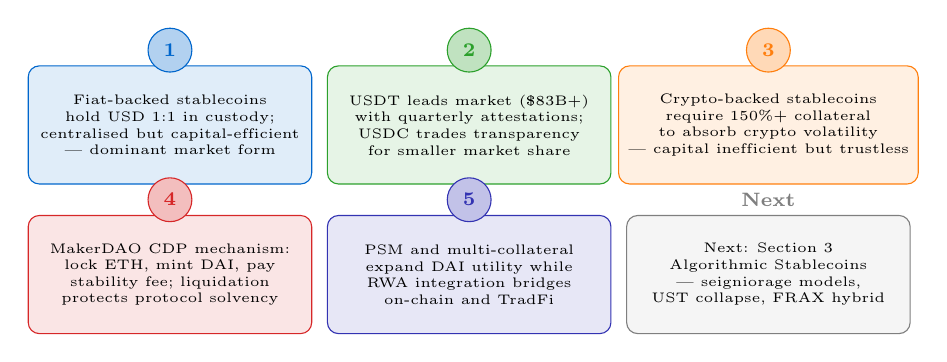
\begin{tikzpicture}
  \node[draw=mlblue, fill=mlblue!12, rounded corners=4pt, minimum width=3.6cm, minimum height=1.5cm, align=center, font=\tiny] (k1) at (1.9,3.2) {Fiat-backed stablecoins\\hold USD 1:1 in custody;\\centralised but capital-efficient\\--- dominant market form};
  \node[circle, draw=mlblue, fill=mlblue!30, minimum size=0.55cm, font=\scriptsize\bfseries, text=mlblue] at (1.9,4.15) {1};

  \node[draw=mlgreen, fill=mlgreen!12, rounded corners=4pt, minimum width=3.6cm, minimum height=1.5cm, align=center, font=\tiny] (k2) at (5.7,3.2) {USDT leads market (\$83B+)\\with quarterly attestations;\\USDC trades transparency\\for smaller market share};
  \node[circle, draw=mlgreen, fill=mlgreen!30, minimum size=0.55cm, font=\scriptsize\bfseries, text=mlgreen] at (5.7,4.15) {2};

  \node[draw=mlorange, fill=mlorange!12, rounded corners=4pt, minimum width=3.6cm, minimum height=1.5cm, align=center, font=\tiny] (k3) at (9.5,3.2) {Crypto-backed stablecoins\\require 150\%+ collateral\\to absorb crypto volatility\\--- capital inefficient but trustless};
  \node[circle, draw=mlorange, fill=mlorange!30, minimum size=0.55cm, font=\scriptsize\bfseries, text=mlorange] at (9.5,4.15) {3};

  \node[draw=mlred, fill=mlred!12, rounded corners=4pt, minimum width=3.6cm, minimum height=1.5cm, align=center, font=\tiny] (k4) at (1.9,1.3) {MakerDAO CDP mechanism:\\lock ETH, mint DAI, pay\\stability fee; liquidation\\protects protocol solvency};
  \node[circle, draw=mlred, fill=mlred!30, minimum size=0.55cm, font=\scriptsize\bfseries, text=mlred] at (1.9,2.25) {4};

  \node[draw=mlpurple, fill=mlpurple!12, rounded corners=4pt, minimum width=3.6cm, minimum height=1.5cm, align=center, font=\tiny] (k5) at (5.7,1.3) {PSM and multi-collateral\\expand DAI utility while\\RWA integration bridges\\on-chain and TradFi};
  \node[circle, draw=mlpurple, fill=mlpurple!30, minimum size=0.55cm, font=\scriptsize\bfseries, text=mlpurple] at (5.7,2.25) {5};

  \node[draw=mlgray, fill=mlgray!8, rounded corners=4pt, minimum width=3.6cm, minimum height=1.5cm, align=center, font=\tiny] (k6) at (9.5,1.3) {Next: Section 3\\Algorithmic Stablecoins\\--- seigniorage models,\\UST collapse, FRAX hybrid};
  \node[font=\scriptsize\bfseries, text=mlgray] at (9.5,2.25) {Next};
\end{tikzpicture}
\bottomnote{Section 2 complete | 5 key takeaways | Proceed to Section 3: Algorithmic Stablecoins for seigniorage models and the UST failure post-mortem}
\end{frame}

%% ============================================================
%% SECTION 3: ALGORITHMIC STABLECOINS
%% ============================================================
\section{Algorithmic Stablecoins}

% Frame 27: Section 3 Divider
\begin{frame}{Section 3: Algorithmic Stablecoins}
\begin{beamercolorbox}[sep=12pt,center,rounded=true,shadow=true]{palette quaternary}
  {\Large\bfseries Section 3: Algorithmic Stablecoins}\\[4pt]
  {\normalsize Achieving price stability through smart contract mechanisms without full collateral}
\end{beamercolorbox}

\vspace{4mm}
\begin{columns}[T]
\column{0.55\textwidth}
\begin{block}{What You Will Learn}
\begin{itemize}\setlength{\itemsep}{2pt}
  \item How algorithmic peg mechanisms work without collateral
  \item Rebasing and seigniorage models compared
  \item Terra/LUNA architecture and the May 2022 collapse
  \item Why most algorithmic stablecoins fail
  \item Hybrid approaches: Frax fractional-algorithmic design
  \item The stablecoin trilemma: stability, efficiency, decentralisation
\end{itemize}
\end{block}
\column{0.45\textwidth}
\begin{block}{Frames in This Section}
\begin{itemize}\setlength{\itemsep}{2pt}
  \item Frame 28: Algorithmic Concept
  \item Frame 29: Rebasing Mechanism (AMPL)
  \item Frame 30: Seigniorage Model
  \item Frame 31: Terra/LUNA Architecture (Code)
  \item Frame 32: Collapse Timeline
  \item Frame 33: Death Spiral Mechanics
  \item Frame 34: Anchor Protocol \& 20\% Yield
  \item Frame 35: Lessons from Failures
  \item Frame 36: Frax Fractional-Algorithmic
  \item Frame 37: Stablecoin Trilemma
  \item Frame 38: Section 3 Summary
\end{itemize}
\end{block}
\end{columns}
\bottomnote{Section 3 of 5 | Frames 27--38 | Algorithmic mechanisms, the UST post-mortem, and hybrid designs}
\end{frame}

% Frame 28: Algorithmic Stablecoin Concept
\begin{frame}{Algorithmic Stablecoin Concept}
\begin{columns}[T]
\column{0.45\textwidth}
\begin{block}{Core Idea}
\begin{itemize}\setlength{\itemsep}{2pt}
  \item \textbf{No collateral required:} Peg maintained purely through supply control
  \item \textbf{Above \$1.00:} Protocol expands supply --- more coins, price falls
  \item \textbf{Below \$1.00:} Protocol contracts supply --- fewer coins, price rises
  \item \textbf{Incentive:} Arbitrageurs profit by exploiting deviations
  \item \textbf{Risk:} Mechanism depends on market confidence; no backstop
\end{itemize}
\end{block}
\vspace{2mm}
\begin{alertblock}{Key Insight}
\scriptsize Algorithmic stablecoins replace collateral with game theory: if everyone believes the peg holds, it holds. When belief breaks, no assets exist to restore it.
\end{alertblock}
\column{0.55\textwidth}
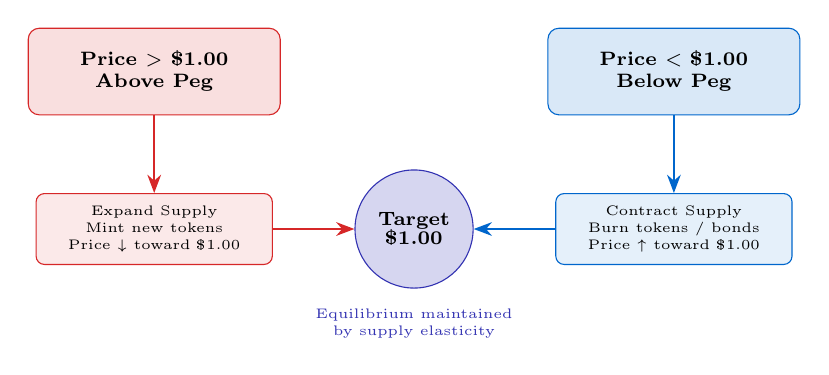
\begin{tikzpicture}
  %% Center target
  \node[draw=mlpurple, fill=mlpurple!20, circle, minimum size=1.5cm, align=center, font=\scriptsize\bfseries] (target) at (5.5,2.8) {Target\\[-1pt]\$1.00};

  %% Above peg box
  \node[draw=mlred, fill=mlred!15, rounded corners=4pt, minimum width=3.2cm, minimum height=1.1cm, align=center, font=\scriptsize\bfseries] (above) at (2.2,4.8) {Price $>$ \$1.00\\Above Peg};

  %% Below peg box
  \node[draw=mlblue, fill=mlblue!15, rounded corners=4pt, minimum width=3.2cm, minimum height=1.1cm, align=center, font=\scriptsize\bfseries] (below) at (8.8,4.8) {Price $<$ \$1.00\\Below Peg};

  %% Actions
  \node[draw=mlred, fill=mlred!10, rounded corners=3pt, minimum width=3.0cm, minimum height=0.9cm, align=center, font=\tiny] (expand) at (2.2,2.8) {Expand Supply\\Mint new tokens\\Price $\downarrow$ toward \$1.00};

  \node[draw=mlblue, fill=mlblue!10, rounded corners=3pt, minimum width=3.0cm, minimum height=0.9cm, align=center, font=\tiny] (contract) at (8.8,2.8) {Contract Supply\\Burn tokens / bonds\\Price $\uparrow$ toward \$1.00};

  %% Arrows
  \draw[-{Stealth}, thick, mlred] (above.south) -- (expand.north);
  \draw[-{Stealth}, thick, mlred] (expand.east) -- (target.west);
  \draw[-{Stealth}, thick, mlblue] (below.south) -- (contract.north);
  \draw[-{Stealth}, thick, mlblue] (contract.west) -- (target.east);

  %% Equilibrium label
  \node[font=\tiny, align=center, text=mlpurple] at (5.5,1.6) {Equilibrium maintained\\by supply elasticity};
\end{tikzpicture}
\end{columns}
\bottomnote{Algorithmic stablecoins: Basis, Empty Set Dollar, Ampleforth, Terra/UST | Combined peak market cap $>$\$60B (May 2022) | All major designs have failed or required collateral backstop}
\end{frame}

% Frame 29: Rebasing Mechanism (Ampleforth)
\begin{frame}{Rebasing Mechanism: Ampleforth (AMPL)}
\begin{columns}[T]
\column{0.48\textwidth}
\begin{block}{How Rebasing Works}
\begin{itemize}\setlength{\itemsep}{2pt}
  \item \textbf{Elastic supply:} All AMPL balances adjust simultaneously every 24h
  \item \textbf{Positive rebase:} Price $>$ \$1.05 --- every wallet balance increases proportionally
  \item \textbf{Negative rebase:} Price $<$ \$0.95 --- every wallet balance decreases proportionally
  \item \textbf{No rebase zone:} \$0.95--\$1.05 --- supply unchanged
  \item \textbf{Key property:} Your \% share of total supply never changes
\end{itemize}
\end{block}
\vspace{2mm}
\begin{exampleblock}{Example: 10,000 AMPL at \$1.10}
\scriptsize
Rebase factor $= \frac{1.10 - 1.00}{0.10} \times 0.10 = +10\%$\\[2pt]
New balance: $10{,}000 \times 1.10 = 11{,}000$ AMPL\\[2pt]
Price target: supply $\uparrow$ pushes price $\downarrow$ to \$1.00
\end{exampleblock}
\column{0.52\textwidth}
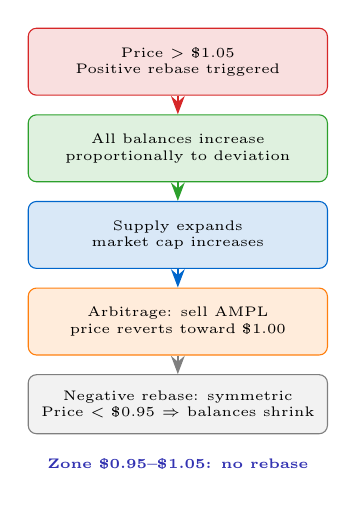
\begin{tikzpicture}
  \node[draw=mlred, fill=mlred!15, rounded corners=3pt, minimum width=3.8cm, minimum height=0.85cm, align=center, font=\tiny]    (s1) at (5.5,5.2) {Price $>$ \$1.05\\Positive rebase triggered};
  \node[draw=mlgreen, fill=mlgreen!15, rounded corners=3pt, minimum width=3.8cm, minimum height=0.85cm, align=center, font=\tiny]  (s2) at (5.5,4.1) {All balances increase\\proportionally to deviation};
  \node[draw=mlblue, fill=mlblue!15, rounded corners=3pt, minimum width=3.8cm, minimum height=0.85cm, align=center, font=\tiny]   (s3) at (5.5,3.0) {Supply expands\\market cap increases};
  \node[draw=mlorange, fill=mlorange!15, rounded corners=3pt, minimum width=3.8cm, minimum height=0.85cm, align=center, font=\tiny] (s4) at (5.5,1.9) {Arbitrage: sell AMPL\\price reverts toward \$1.00};

  \node[draw=mlgray, fill=mlgray!10, rounded corners=3pt, minimum width=3.8cm, minimum height=0.75cm, align=center, font=\tiny] (s5) at (5.5,0.85) {Negative rebase: symmetric\\Price $<$ \$0.95 $\Rightarrow$ balances shrink};

  \draw[-{Stealth}, thick, mlred]    (s1.south) -- (s2.north);
  \draw[-{Stealth}, thick, mlgreen]  (s2.south) -- (s3.north);
  \draw[-{Stealth}, thick, mlblue]   (s3.south) -- (s4.north);
  \draw[-{Stealth}, thick, mlgray]   (s4.south) -- (s5.north);

  \node[font=\tiny\bfseries, text=mlpurple] at (5.5,0.1) {Zone \$0.95--\$1.05: no rebase};
\end{tikzpicture}
\end{columns}
\bottomnote{AMPL launched 2019 | Peak market cap \$800M (Jul 2020) | Rebasing does not guarantee price stability --- supply elasticity shifts purchasing power not price | AMPL remains live but niche}
\end{frame}

% Frame 30: Seigniorage Model
\begin{frame}{Seigniorage Model: Two-Token Design}
\begin{columns}[T]
\column{0.46\textwidth}
\begin{block}{Seigniorage Mechanics}
\begin{itemize}\setlength{\itemsep}{2pt}
  \item \textbf{Two tokens:} Stablecoin (pegged) + Governance/seigniorage token (volatile)
  \item \textbf{Expansion:} When stablecoin $>$ \$1, mint new stablecoins and distribute to governance holders
  \item \textbf{Contraction:} When stablecoin $<$ \$1, sell bonds/coupons to absorb supply
  \item \textbf{Arbitrage loop:} Burn 1 governance token to mint \$1 of stablecoin; or redeem \$1 stablecoin for \$1 governance token
  \item \textbf{Stability assumption:} Governance token must retain value to back the peg
\end{itemize}
\end{block}
\vspace{2mm}
\begin{alertblock}{Fatal Flaw}
\scriptsize If governance token price collapses, the mint/burn arbitrage loop becomes unprofitable, destroying the peg mechanism entirely.
\end{alertblock}
\column{0.54\textwidth}
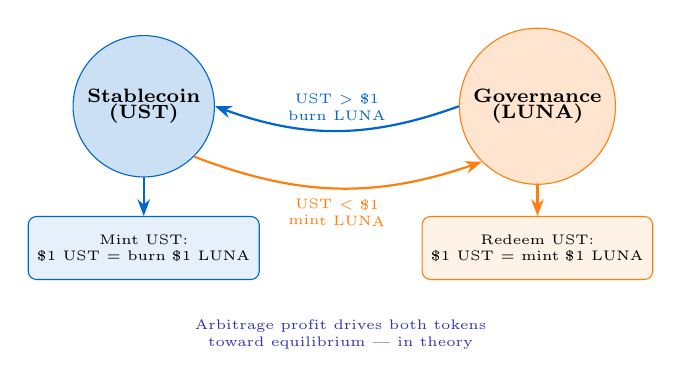
\begin{tikzpicture}
  %% Tokens
  \node[draw=mlblue, fill=mlblue!20, circle, minimum size=1.6cm, align=center, font=\scriptsize\bfseries]   (ust)  at (3.0,3.6) {Stablecoin\\[-2pt](UST)};
  \node[draw=mlorange, fill=mlorange!20, circle, minimum size=1.6cm, align=center, font=\scriptsize\bfseries] (luna) at (8.0,3.6) {Governance\\[-2pt](LUNA)};

  %% Actions
  \node[draw=mlblue, fill=mlblue!10, rounded corners=3pt, minimum width=2.8cm, minimum height=0.8cm, align=center, font=\tiny]   (mint)  at (3.0,1.8) {Mint UST:\\\$1 UST = burn \$1 LUNA};
  \node[draw=mlorange, fill=mlorange!10, rounded corners=3pt, minimum width=2.8cm, minimum height=0.8cm, align=center, font=\tiny] (redeem) at (8.0,1.8) {Redeem UST:\\\$1 UST = mint \$1 LUNA};

  %% Above peg arrow
  \draw[-{Stealth[length=6pt]}, thick, mlblue, bend left=20] (luna.west) to node[font=\tiny, align=center, text=mlblue, above, sloped]{UST $>$ \$1\\burn LUNA} (ust.east);

  %% Below peg arrow
  \draw[-{Stealth[length=6pt]}, thick, mlorange, bend right=20] (ust.south east) to node[font=\tiny, align=center, text=mlorange, below, sloped]{UST $<$ \$1\\mint LUNA} (luna.south west);

  \draw[-{Stealth[length=6pt]}, thick, mlblue]   (ust.south)  -- (mint.north);
  \draw[-{Stealth[length=6pt]}, thick, mlorange] (luna.south) -- (redeem.north);

  \node[font=\tiny, align=center, text=mlpurple] at (5.5,0.7) {Arbitrage profit drives both tokens\\toward equilibrium --- in theory};
\end{tikzpicture}
\end{columns}
\bottomnote{Seigniorage models: Basis (shutdown 2018), Terra/LUNA (collapsed 2022), Olympus DAO (fragile) | Two-token design popular 2020--2022 | All major implementations ultimately failed}
\end{frame}

% Frame 31: Terra/LUNA Architecture [FRAGILE] -- CODE FRAME 2
\begin{frame}[fragile]{Terra/LUNA Architecture}
\begin{columns}[T]
\column{0.52\textwidth}
\begin{lstlisting}[language=Solidity, caption={Simplified Terra Swap Logic}]
// Simplified Terra swap logic
contract TerraSwap {
    uint256 public ustSupply;
    uint256 public lunaPrice;

    // Mint UST by burning LUNA
    function mintUST(uint256 lunaAmount)
        external {
        uint256 ustAmount = lunaAmount
            * lunaPrice / 1e18;
        ustSupply += ustAmount;
        // burn lunaAmount from sender
    }

    // Redeem UST for LUNA
    function redeemUST(uint256 ustAmount)
        external {
        uint256 lunaAmount = ustAmount
            * 1e18 / lunaPrice;
        ustSupply -= ustAmount;
        // mint lunaAmount to sender
    }
}
\end{lstlisting}
\column{0.48\textwidth}
\begin{block}{Arbitrage Mechanism}
\begin{itemize}\setlength{\itemsep}{3pt}
  \item \textbf{UST $>$ \$1:} Burn \$1 of LUNA, receive 1 UST; sell UST for $>$\$1; pocket profit
  \item \textbf{UST $<$ \$1:} Buy 1 UST for $<$\$1; burn UST, receive \$1 LUNA; pocket spread
  \item \textbf{lunaPrice oracle:} Updated by Terra validators; manipulation risk
  \item \textbf{ustSupply:} Unbounded growth possible if LUNA price rises fast
  \item \textbf{Critical path:} Arbitrage only works if LUNA has positive market value
\end{itemize}
\end{block}
\vspace{2mm}
\begin{alertblock}{Design Vulnerability}
\scriptsize When LUNA price falls rapidly, arbitrageurs must receive ever-increasing LUNA quantities per UST redeemed --- hyperinflating LUNA supply and accelerating price collapse.
\end{alertblock}
\end{columns}
\bottomnote{Terra blockchain: Cosmos SDK, native LUNA token | UST peak supply: \$18.7B (May 2022) | Mint/burn module: terra/market | Oracle manipulation resistance: weighted median from 30+ validators}
\end{frame}

% Frame 32: Terra/LUNA Collapse Timeline
\begin{frame}{Terra/LUNA Collapse Timeline: May 2022}
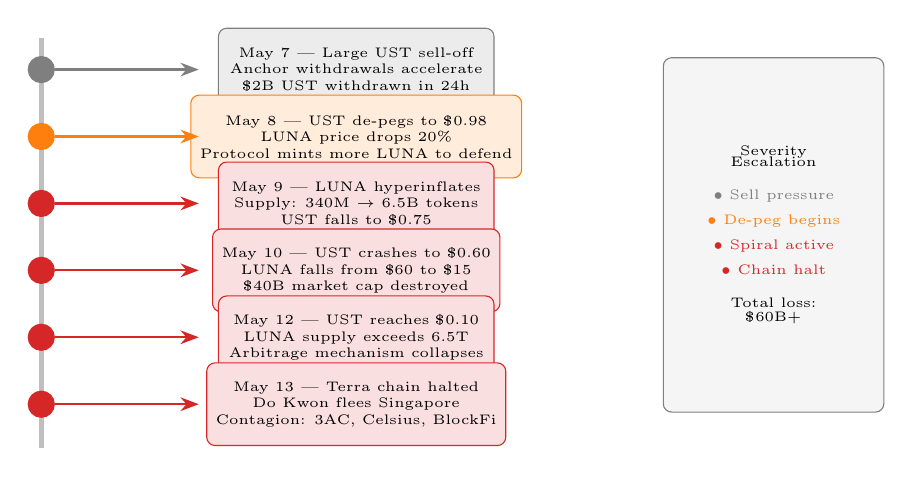
\begin{tikzpicture}
  %% Timeline spine
  \draw[line width=2pt, mlgray!50] (0.5,0.4) -- (0.5,5.6);

  %% Event 1 -- May 7
  \node[circle, draw=mlgray, fill=mlgray, minimum size=0.28cm]   (d1) at (0.5,5.2) {};
  \node[draw=mlgray, fill=mlgray!15, rounded corners=3pt, minimum width=3.5cm, minimum height=1.05cm, align=center, font=\tiny]   at (4.5,5.2) {May 7 | Large UST sell-off\\Anchor withdrawals accelerate\\\$2B UST withdrawn in 24h};
  \draw[-{Stealth}, thick, mlgray]   (d1.east) -- (2.5,5.2);

  %% Event 2 -- May 8
  \node[circle, draw=mlorange, fill=mlorange, minimum size=0.28cm] (d2) at (0.5,4.35) {};
  \node[draw=mlorange, fill=mlorange!15, rounded corners=3pt, minimum width=3.5cm, minimum height=1.05cm, align=center, font=\tiny] at (4.5,4.35) {May 8 | UST de-pegs to \$0.98\\LUNA price drops 20\%\\Protocol mints more LUNA to defend};
  \draw[-{Stealth}, thick, mlorange] (d2.east) -- (2.5,4.35);

  %% Event 3 -- May 9
  \node[circle, draw=mlred, fill=mlred, minimum size=0.28cm]    (d3) at (0.5,3.5) {};
  \node[draw=mlred, fill=mlred!15, rounded corners=3pt, minimum width=3.5cm, minimum height=1.05cm, align=center, font=\tiny]    at (4.5,3.5) {May 9 | LUNA hyperinflates\\Supply: 340M $\to$ 6.5B tokens\\UST falls to \$0.75};
  \draw[-{Stealth}, thick, mlred]    (d3.east) -- (2.5,3.5);

  %% Event 4 -- May 10
  \node[circle, draw=mlred, fill=mlred, minimum size=0.28cm]    (d4) at (0.5,2.65) {};
  \node[draw=mlred, fill=mlred!15, rounded corners=3pt, minimum width=3.5cm, minimum height=1.05cm, align=center, font=\tiny]    at (4.5,2.65) {May 10 | UST crashes to \$0.60\\LUNA falls from \$60 to \$15\\\$40B market cap destroyed};
  \draw[-{Stealth}, thick, mlred]    (d4.east) -- (2.5,2.65);

  %% Event 5 -- May 12
  \node[circle, draw=mlred, fill=mlred, minimum size=0.28cm]    (d5) at (0.5,1.8) {};
  \node[draw=mlred, fill=mlred!15, rounded corners=3pt, minimum width=3.5cm, minimum height=1.05cm, align=center, font=\tiny]    at (4.5,1.8) {May 12 | UST reaches \$0.10\\LUNA supply exceeds 6.5T\\Arbitrage mechanism collapses};
  \draw[-{Stealth}, thick, mlred]    (d5.east) -- (2.5,1.8);

  %% Event 6 -- May 13
  \node[circle, draw=mlred, fill=mlred, minimum size=0.28cm]    (d6) at (0.5,0.95) {};
  \node[draw=mlred, fill=mlred!15, rounded corners=3pt, minimum width=3.5cm, minimum height=1.05cm, align=center, font=\tiny]    at (4.5,0.95) {May 13 | Terra chain halted\\Do Kwon flees Singapore\\Contagion: 3AC, Celsius, BlockFi};
  \draw[-{Stealth}, thick, mlred]    (d6.east) -- (2.5,0.95);

  %% Right: severity legend
  \node[draw=mlgray, fill=mlgray!8, rounded corners=3pt, minimum width=2.8cm, minimum height=4.5cm, align=center, font=\tiny] at (9.8,3.1) {Severity\\[-2pt]{\tiny Escalation}\\[6pt]
  \textcolor{mlgray}{$\bullet$ Sell pressure}\\[3pt]
  \textcolor{mlorange}{$\bullet$ De-peg begins}\\[3pt]
  \textcolor{mlred}{$\bullet$ Spiral active}\\[3pt]
  \textcolor{mlred}{$\bullet$ Chain halt}\\[6pt]
  Total loss:\\[-1pt]\$60B+};
\end{tikzpicture}
\bottomnote{Total value destroyed: \$60B+ | LUNA: \$119 peak (Apr 5) to \$0.0002 (May 13) | UST: \$18.7B supply to \$0 | Do Kwon indicted by US DOJ (2023) | Largest crypto collapse in history}
\end{frame}

% Frame 33: Death Spiral Mechanics
\begin{frame}{Death Spiral Mechanics}
\begin{columns}[T]
\column{0.44\textwidth}
\begin{block}{Why Spirals Are Inevitable}
\begin{itemize}\setlength{\itemsep}{2pt}
  \item \textbf{Reflexivity:} Falling LUNA price makes UST defence more expensive
  \item \textbf{Dilution:} Each UST redeemed mints more LUNA, diluting existing holders
  \item \textbf{Confidence:} Rational actors exit before others, accelerating collapse
  \item \textbf{No floor:} Unlike crypto-backed, no collateral to liquidate for recovery
  \item \textbf{Bank run dynamics:} Game theory favours early exit for all participants
\end{itemize}
\end{block}
\vspace{2mm}
\begin{alertblock}{Nash Equilibrium}
\scriptsize Once confidence wavers, the dominant strategy for every holder is to exit immediately. This creates a self-fulfilling prophecy that guarantees collapse.
\end{alertblock}
\column{0.56\textwidth}
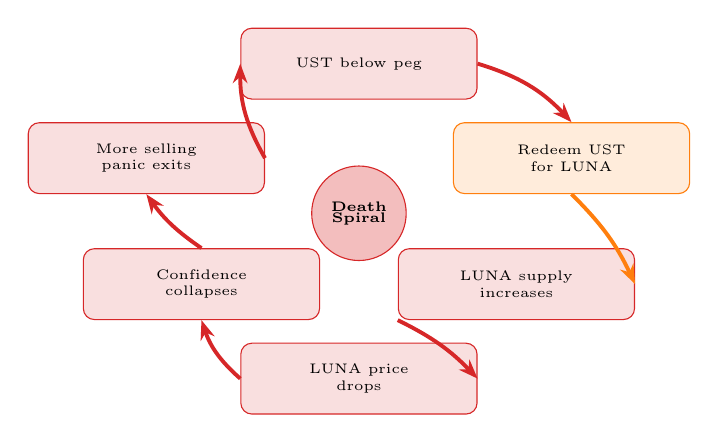
\begin{tikzpicture}
  %% Circular nodes
  \node[draw=mlred, fill=mlred!15, rounded corners=4pt, minimum width=3.0cm, minimum height=0.9cm, align=center, font=\tiny]    (a) at (5.5,5.0) {UST below peg};
  \node[draw=mlorange, fill=mlorange!15, rounded corners=4pt, minimum width=3.0cm, minimum height=0.9cm, align=center, font=\tiny] (b) at (8.2,3.8) {Redeem UST\\for LUNA};
  \node[draw=mlred, fill=mlred!15, rounded corners=4pt, minimum width=3.0cm, minimum height=0.9cm, align=center, font=\tiny]    (c) at (7.5,2.2) {LUNA supply\\increases};
  \node[draw=mlred, fill=mlred!15, rounded corners=4pt, minimum width=3.0cm, minimum height=0.9cm, align=center, font=\tiny]    (d) at (5.5,1.0) {LUNA price\\drops};
  \node[draw=mlred, fill=mlred!15, rounded corners=4pt, minimum width=3.0cm, minimum height=0.9cm, align=center, font=\tiny]    (e) at (3.5,2.2) {Confidence\\collapses};
  \node[draw=mlred, fill=mlred!15, rounded corners=4pt, minimum width=3.0cm, minimum height=0.9cm, align=center, font=\tiny]    (f) at (2.8,3.8) {More selling\\panic exits};

  %% Circular arrows
  \draw[-{Stealth[length=7pt]}, line width=1.4pt, mlred]    (a.east)  to[bend left=15]  (b.north);
  \draw[-{Stealth[length=7pt]}, line width=1.4pt, mlorange] (b.south) to[bend left=10]  (c.east);
  \draw[-{Stealth[length=7pt]}, line width=1.4pt, mlred]    (c.south west) to[bend left=10]  (d.east);
  \draw[-{Stealth[length=7pt]}, line width=1.4pt, mlred]    (d.west)  to[bend left=15]  (e.south);
  \draw[-{Stealth[length=7pt]}, line width=1.4pt, mlred]    (e.north) to[bend left=10]  (f.south);
  \draw[-{Stealth[length=7pt]}, line width=1.4pt, mlred]    (f.east)  to[bend left=15]  (a.west);

  %% Centre label
  \node[draw=mlred, fill=mlred!30, circle, minimum size=1.2cm, align=center, font=\tiny\bfseries] at (5.5,3.1) {Death\\[-2pt]Spiral};
\end{tikzpicture}
\end{columns}
\bottomnote{Death spiral: positive feedback loop where each step amplifies the next | First described in context of currency attacks (Soros/GBP 1992) | Applies to any undercollateralised peg system | No known algorithmic fix}
\end{frame}

% Frame 34: Anchor Protocol and the 20% Yield
\begin{frame}{Anchor Protocol and the 20\% APY Problem}
\begin{columns}[T]
\column{0.48\textwidth}
\begin{block}{How Anchor Offered $\approx$20\% APY}
\begin{itemize}\setlength{\itemsep}{2pt}
  \item \textbf{Mechanism:} Deposit UST, receive aUST bearing yield
  \item \textbf{Collateral:} Borrowers deposit bLUNA/bETH (staked assets) as collateral
  \item \textbf{Yield source 1:} Borrower interest payments (variable, $\approx$12\%)
  \item \textbf{Yield source 2:} Staking rewards from bLUNA/bETH collateral ($\approx$6-8\%)
  \item \textbf{Yield source 3:} Luna Foundation Guard (LFG) subsidised shortfall from reserves
  \item \textbf{Reality:} Subsidies burned through \$450M reserve in 3 months
\end{itemize}
\end{block}
\vspace{2mm}
\begin{alertblock}{Warning Signal}
\scriptsize Anchor paid depositors more than borrowers paid in interest. The \$450M reserve was a time-limited subsidy, not sustainable yield.
\end{alertblock}
\column{0.52\textwidth}
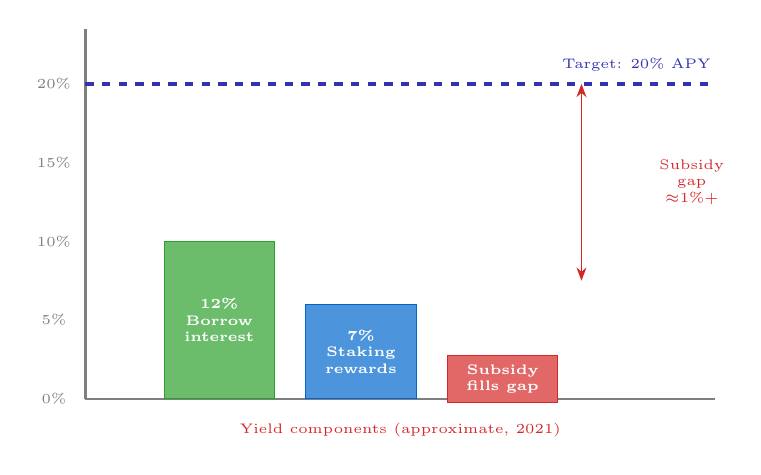
\begin{tikzpicture}
  %% Axes
  \draw[thick, mlgray] (1.5,0.5) -- (1.5,5.2);
  \draw[thick, mlgray] (1.5,0.5) -- (9.5,0.5);

  %% Bars: Yield components
  \node[draw=mlgreen, fill=mlgreen!70, minimum width=1.4cm, minimum height=2.0cm, align=center, font=\tiny\bfseries, text=white] at (3.2,1.5) {12\%\\Borrow\\interest};
  \node[draw=mlblue, fill=mlblue!70, minimum width=1.4cm, minimum height=1.2cm, align=center, font=\tiny\bfseries, text=white]  at (5.0,1.1) {7\%\\Staking\\rewards};
  \node[draw=mlred, fill=mlred!70, minimum width=1.4cm, minimum height=0.5cm, align=center, font=\tiny\bfseries, text=white]   at (6.8,0.75) {Subsidy\\fills gap};

  %% Total target line
  \draw[dashed, mlpurple, line width=1.2pt] (1.5,4.5) -- (9.5,4.5);
  \node[font=\tiny, align=center, text=mlpurple] at (8.5,4.75) {Target: 20\% APY};

  %% Gap annotation
  \draw[{Stealth}-{Stealth}, mlred] (7.8,2.0) -- (7.8,4.5);
  \node[font=\tiny, align=center, text=mlred] at (9.2,3.25) {Subsidy\\gap\\$\approx$1\%+};

  %% Y-axis labels
  \node[font=\tiny, align=center, text=mlgray] at (1.1,0.5) {\tiny 0\%};
  \node[font=\tiny, align=center, text=mlgray] at (1.1,1.5) {\tiny 5\%};
  \node[font=\tiny, align=center, text=mlgray] at (1.1,2.5) {\tiny 10\%};
  \node[font=\tiny, align=center, text=mlgray] at (1.1,3.5) {\tiny 15\%};
  \node[font=\tiny, align=center, text=mlgray] at (1.1,4.5) {\tiny 20\%};

  \node[font=\tiny, align=center, text=mlred] at (5.5,0.1) {Yield components (approximate, 2021)};
\end{tikzpicture}
\end{columns}
\bottomnote{Anchor Protocol: \$14B TVL at peak (Mar 2022) | LFG reserve: \$450M depleted in $<$90 days | 20\% APY attracted 72\% of all UST supply | Unsustainable yield primary driver of UST demand and subsequent collapse}
\end{frame}

% Frame 35: Lessons from Algorithmic Failures
\begin{frame}{Lessons from Algorithmic Stablecoin Failures}
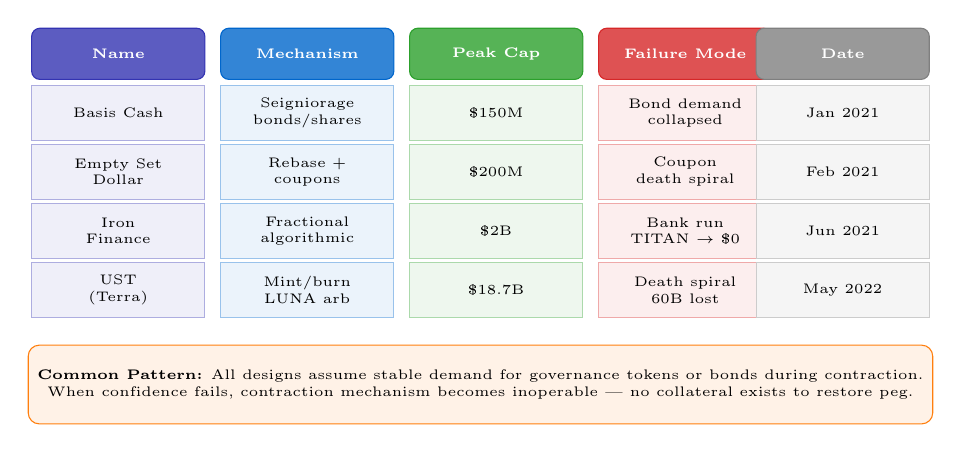
\begin{tikzpicture}
  %% Column headers
  \node[draw=mlpurple, fill=mlpurple!80, rounded corners=3pt, minimum width=2.2cm, minimum height=0.65cm, align=center, font=\tiny\bfseries, text=white] at (1.3,5.3) {Name};
  \node[draw=mlblue, fill=mlblue!80, rounded corners=3pt, minimum width=2.2cm, minimum height=0.65cm, align=center, font=\tiny\bfseries, text=white]   at (3.7,5.3) {Mechanism};
  \node[draw=mlgreen, fill=mlgreen!80, rounded corners=3pt, minimum width=2.2cm, minimum height=0.65cm, align=center, font=\tiny\bfseries, text=white]  at (6.1,5.3) {Peak Cap};
  \node[draw=mlred, fill=mlred!80, rounded corners=3pt, minimum width=2.2cm, minimum height=0.65cm, align=center, font=\tiny\bfseries, text=white]    at (8.5,5.3) {Failure Mode};
  \node[draw=mlgray, fill=mlgray!80, rounded corners=3pt, minimum width=2.2cm, minimum height=0.65cm, align=center, font=\tiny\bfseries, text=white]   at (10.5,5.3) {Date};

  %% Row 1: Basis Cash
  \node[draw=mlpurple!40, fill=mlpurple!8, minimum width=2.2cm, minimum height=0.7cm, align=center, font=\tiny] at (1.3,4.55) {Basis Cash};
  \node[draw=mlblue!40, fill=mlblue!8, minimum width=2.2cm, minimum height=0.7cm, align=center, font=\tiny]   at (3.7,4.55) {Seigniorage\\bonds/shares};
  \node[draw=mlgreen!40, fill=mlgreen!8, minimum width=2.2cm, minimum height=0.7cm, align=center, font=\tiny]  at (6.1,4.55) {\$150M};
  \node[draw=mlred!40, fill=mlred!8, minimum width=2.2cm, minimum height=0.7cm, align=center, font=\tiny]    at (8.5,4.55) {Bond demand\\collapsed};
  \node[draw=mlgray!40, fill=mlgray!8, minimum width=2.2cm, minimum height=0.7cm, align=center, font=\tiny]   at (10.5,4.55) {Jan 2021};

  %% Row 2: Empty Set Dollar
  \node[draw=mlpurple!40, fill=mlpurple!8, minimum width=2.2cm, minimum height=0.7cm, align=center, font=\tiny] at (1.3,3.8) {Empty Set\\Dollar};
  \node[draw=mlblue!40, fill=mlblue!8, minimum width=2.2cm, minimum height=0.7cm, align=center, font=\tiny]   at (3.7,3.8) {Rebase +\\coupons};
  \node[draw=mlgreen!40, fill=mlgreen!8, minimum width=2.2cm, minimum height=0.7cm, align=center, font=\tiny]  at (6.1,3.8) {\$200M};
  \node[draw=mlred!40, fill=mlred!8, minimum width=2.2cm, minimum height=0.7cm, align=center, font=\tiny]    at (8.5,3.8) {Coupon\\death spiral};
  \node[draw=mlgray!40, fill=mlgray!8, minimum width=2.2cm, minimum height=0.7cm, align=center, font=\tiny]   at (10.5,3.8) {Feb 2021};

  %% Row 3: Iron Finance
  \node[draw=mlpurple!40, fill=mlpurple!8, minimum width=2.2cm, minimum height=0.7cm, align=center, font=\tiny] at (1.3,3.05) {Iron\\Finance};
  \node[draw=mlblue!40, fill=mlblue!8, minimum width=2.2cm, minimum height=0.7cm, align=center, font=\tiny]   at (3.7,3.05) {Fractional\\algorithmic};
  \node[draw=mlgreen!40, fill=mlgreen!8, minimum width=2.2cm, minimum height=0.7cm, align=center, font=\tiny]  at (6.1,3.05) {\$2B};
  \node[draw=mlred!40, fill=mlred!8, minimum width=2.2cm, minimum height=0.7cm, align=center, font=\tiny]    at (8.5,3.05) {Bank run\\TITAN $\to$ \$0};
  \node[draw=mlgray!40, fill=mlgray!8, minimum width=2.2cm, minimum height=0.7cm, align=center, font=\tiny]   at (10.5,3.05) {Jun 2021};

  %% Row 4: UST
  \node[draw=mlpurple!40, fill=mlpurple!8, minimum width=2.2cm, minimum height=0.7cm, align=center, font=\tiny] at (1.3,2.3) {UST\\(Terra)};
  \node[draw=mlblue!40, fill=mlblue!8, minimum width=2.2cm, minimum height=0.7cm, align=center, font=\tiny]   at (3.7,2.3) {Mint/burn\\LUNA arb};
  \node[draw=mlgreen!40, fill=mlgreen!8, minimum width=2.2cm, minimum height=0.7cm, align=center, font=\tiny]  at (6.1,2.3) {\$18.7B};
  \node[draw=mlred!40, fill=mlred!8, minimum width=2.2cm, minimum height=0.7cm, align=center, font=\tiny]    at (8.5,2.3) {Death spiral\\60B lost};
  \node[draw=mlgray!40, fill=mlgray!8, minimum width=2.2cm, minimum height=0.7cm, align=center, font=\tiny]   at (10.5,2.3) {May 2022};

  %% Lesson box
  \node[draw=mlorange, fill=mlorange!10, rounded corners=4pt, minimum width=10.5cm, minimum height=1.0cm, align=center, font=\tiny] at (5.9,1.1)
    {\textbf{Common Pattern:} All designs assume stable demand for governance tokens or bonds during contraction.\\When confidence fails, contraction mechanism becomes inoperable --- no collateral exists to restore peg.};
\end{tikzpicture}
\bottomnote{Failed algorithmic stablecoins: 100\% failure rate for pure designs | Combined losses: $>$\$70B | Iron Finance: Mark Cuban investor | Pattern: works in bull markets, fails catastrophically in downturns}
\end{frame}

% Frame 36: Fractional-Algorithmic Approach (Frax)
\begin{frame}{Fractional-Algorithmic Approach: Frax}
\begin{columns}[T]
\column{0.46\textwidth}
\begin{block}{Frax Hybrid Design}
\begin{itemize}\setlength{\itemsep}{2pt}
  \item \textbf{Two tokens:} FRAX (stablecoin) + FXS (Frax Shares, governance)
  \item \textbf{Collateral ratio (CR):} Adjustable 0--100\%; starts at 100\% USDC
  \item \textbf{Expansion:} If FRAX $>$ \$1, CR decreases (less collateral needed)
  \item \textbf{Contraction:} If FRAX $<$ \$1, CR increases (more collateral required)
  \item \textbf{Mint:} Deposit \$CR of USDC + burn \$(1-CR) of FXS to receive 1 FRAX
  \item \textbf{Redeem:} Burn 1 FRAX, receive \$CR of USDC + \$(1-CR) of FXS
\end{itemize}
\end{block}
\vspace{2mm}
\begin{block}{Key Advantage vs.\ Pure Algorithmic}
\scriptsize Collateral provides a floor. Even at 10\% CR, \$0.10 of real assets backs each FRAX, limiting maximum downside unlike UST's zero-collateral model.
\end{block}
\column{0.54\textwidth}
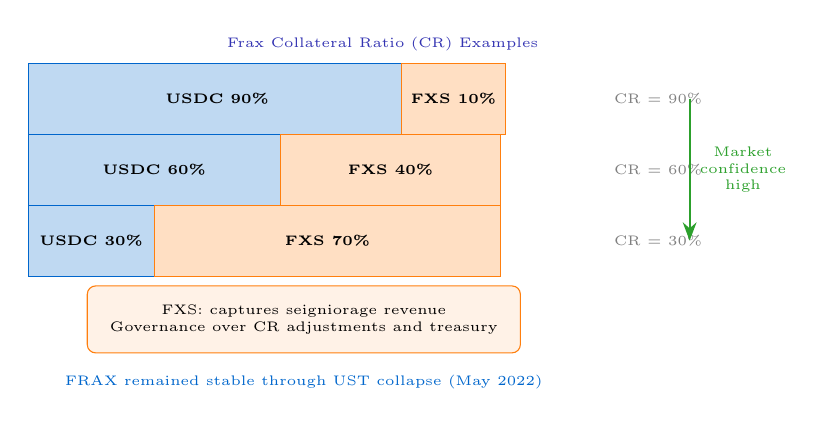
\begin{tikzpicture}
  %% Frax composition bar at different CR levels
  %% CR = 90%
  \node[font=\tiny, align=center, text=mlpurple] at (5.5,5.0) {Frax Collateral Ratio (CR) Examples};

  \node[draw=mlblue, fill=mlblue!25, minimum width=4.8cm, minimum height=0.9cm, align=center, font=\tiny\bfseries] at (3.4,4.3) {USDC 90\%};
  \node[draw=mlorange, fill=mlorange!25, minimum width=1.2cm, minimum height=0.9cm, align=center, font=\tiny\bfseries] at (6.4,4.3) {FXS 10\%};
  \node[font=\tiny, align=center, text=mlgray] at (9.0,4.3) {CR = 90\%};

  \node[draw=mlblue, fill=mlblue!25, minimum width=3.2cm, minimum height=0.9cm, align=center, font=\tiny\bfseries] at (2.6,3.4) {USDC 60\%};
  \node[draw=mlorange, fill=mlorange!25, minimum width=2.8cm, minimum height=0.9cm, align=center, font=\tiny\bfseries] at (5.6,3.4) {FXS 40\%};
  \node[font=\tiny, align=center, text=mlgray] at (9.0,3.4) {CR = 60\%};

  \node[draw=mlblue, fill=mlblue!25, minimum width=1.6cm, minimum height=0.9cm, align=center, font=\tiny\bfseries] at (1.8,2.5) {USDC 30\%};
  \node[draw=mlorange, fill=mlorange!25, minimum width=4.4cm, minimum height=0.9cm, align=center, font=\tiny\bfseries] at (4.8,2.5) {FXS 70\%};
  \node[font=\tiny, align=center, text=mlgray] at (9.0,2.5) {CR = 30\%};

  %% Arrows showing direction
  \draw[-{Stealth}, thick, mlgreen] (9.4,4.3) -- node[font=\tiny, align=center, text=mlgreen, right]{Market\\confidence\\high} (9.4,2.5);

  %% FXS governance label
  \node[draw=mlorange, fill=mlorange!10, rounded corners=3pt, minimum width=5.5cm, minimum height=0.85cm, align=center, font=\tiny] at (4.5,1.5)
    {FXS: captures seigniorage revenue\\Governance over CR adjustments and treasury};

  \node[font=\tiny, align=center, text=mlblue] at (4.5,0.7) {FRAX remained stable through UST collapse (May 2022)};
\end{tikzpicture}
\end{columns}
\bottomnote{Frax Finance launched Dec 2020 | Peak FRAX supply \$3B (2022) | CR dynamically adjusts via PID controller | FRAX maintained peg through UST collapse | FXS market cap: \$500M+ | Most robust algorithmic design to date}
\end{frame}

% Frame 37: Stablecoin Trilemma
\begin{frame}{The Stablecoin Trilemma}
\begin{columns}[T]
\column{0.44\textwidth}
\begin{block}{Three Desiderata}
\begin{itemize}\setlength{\itemsep}{2pt}
  \item \textbf{Price Stability:} Peg holds under stress; low deviation; rapid recovery
  \item \textbf{Capital Efficiency:} Low collateral per \$1 issued; scalable supply
  \item \textbf{Decentralisation:} No trusted custodian; censorship-resistant; permissionless
  \item \textbf{Trilemma:} Achieving all three simultaneously appears impossible
  \item \textbf{USDC:} Stable + efficient, but centralised (Circle can freeze)
  \item \textbf{DAI:} Stable + decentralised, but capital-inefficient (150\%+ collateral)
  \item \textbf{UST:} Efficient + decentralised, but fatally unstable
\end{itemize}
\end{block}
\vspace{2mm}
\begin{alertblock}{Open Research Problem}
\scriptsize No stablecoin has achieved all three properties. FRAX attempts the middle ground with adjustable CR, but retains partial centralisation via USDC collateral.
\end{alertblock}
\column{0.56\textwidth}
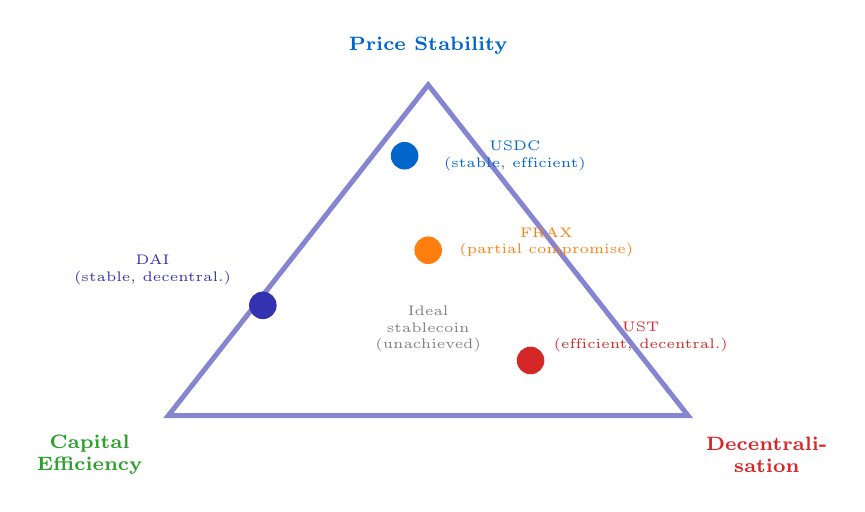
\begin{tikzpicture}
  %% Triangle vertices
  \coordinate (top) at (5.5,5.2);
  \coordinate (bl)  at (2.2,1.0);
  \coordinate (br)  at (8.8,1.0);

  %% Triangle
  \draw[line width=1.8pt, mlpurple!60] (top) -- (bl) -- (br) -- cycle;

  %% Vertex labels
  \node[font=\scriptsize\bfseries, text=mlblue, align=center]   at (5.5,5.7)  {Price Stability};
  \node[font=\scriptsize\bfseries, text=mlgreen, align=center]  at (1.2,0.5)  {Capital\\Efficiency};
  \node[font=\scriptsize\bfseries, text=mlred, align=center]    at (9.8,0.5)  {Decentrali-\\sation};

  %% USDC -- stable + efficient, centralised
  \node[circle, fill=mlblue, minimum size=0.35cm]   (usdc) at (5.2,4.3) {};
  \node[font=\tiny, text=mlblue, align=center]  at (6.6,4.3) {USDC\\(stable, efficient)};

  %% DAI -- stable + decentralised, inefficient
  \node[circle, fill=mlpurple, minimum size=0.35cm] (dai)  at (3.4,2.4) {};
  \node[font=\tiny, text=mlpurple, align=center] at (2.0,2.85) {DAI\\(stable, decentral.)};

  %% UST -- efficient + decentralised, unstable
  \node[circle, fill=mlred, minimum size=0.35cm]    (ust)  at (6.8,1.7) {};
  \node[font=\tiny, text=mlred, align=center]   at (8.2,2.0)  {UST\\(efficient, decentral.)};

  %% FRAX -- middle ground
  \node[circle, fill=mlorange, minimum size=0.35cm] (frax) at (5.5,3.1) {};
  \node[font=\tiny, text=mlorange, align=center] at (7.0,3.2) {FRAX\\(partial compromise)};

  %% Centre label
  \node[font=\tiny, text=mlgray, align=center] at (5.5,2.1) {Ideal\\stablecoin\\(unachieved)};
\end{tikzpicture}
\end{columns}
\bottomnote{Stablecoin trilemma: analogous to blockchain scalability trilemma | First formalised by Ariah Klages-Mundt (2020) | FRAX v3 explores CDP model to reduce USDC dependency | No provably optimal design exists}
\end{frame}

% Frame 38: Section 3 Summary
\begin{frame}{Section 3 Summary}
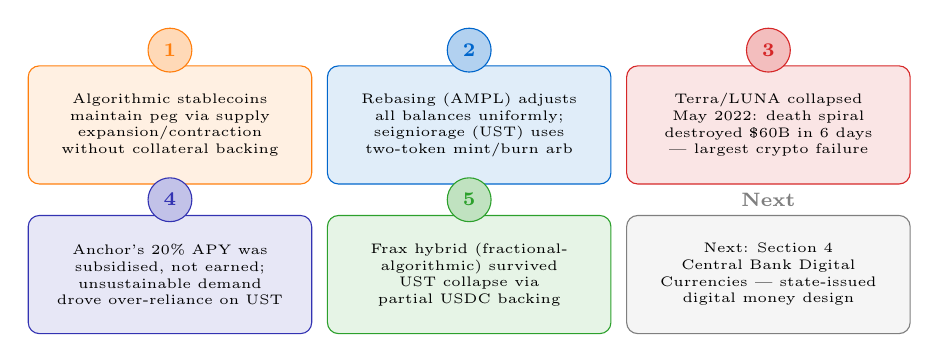
\begin{tikzpicture}
  \node[draw=mlorange, fill=mlorange!12, rounded corners=4pt, minimum width=3.6cm, minimum height=1.5cm, align=center, font=\tiny] (k1) at (1.9,3.2) {Algorithmic stablecoins\\maintain peg via supply\\expansion/contraction\\without collateral backing};
  \node[circle, draw=mlorange, fill=mlorange!30, minimum size=0.55cm, font=\scriptsize\bfseries, text=mlorange] at (1.9,4.15) {1};

  \node[draw=mlblue, fill=mlblue!12, rounded corners=4pt, minimum width=3.6cm, minimum height=1.5cm, align=center, font=\tiny] (k2) at (5.7,3.2) {Rebasing (AMPL) adjusts\\all balances uniformly;\\seigniorage (UST) uses\\two-token mint/burn arb};
  \node[circle, draw=mlblue, fill=mlblue!30, minimum size=0.55cm, font=\scriptsize\bfseries, text=mlblue] at (5.7,4.15) {2};

  \node[draw=mlred, fill=mlred!12, rounded corners=4pt, minimum width=3.6cm, minimum height=1.5cm, align=center, font=\tiny] (k3) at (9.5,3.2) {Terra/LUNA collapsed\\May 2022: death spiral\\destroyed \$60B in 6 days\\--- largest crypto failure};
  \node[circle, draw=mlred, fill=mlred!30, minimum size=0.55cm, font=\scriptsize\bfseries, text=mlred] at (9.5,4.15) {3};

  \node[draw=mlpurple, fill=mlpurple!12, rounded corners=4pt, minimum width=3.6cm, minimum height=1.5cm, align=center, font=\tiny] (k4) at (1.9,1.3) {Anchor's 20\% APY was\\subsidised, not earned;\\unsustainable demand\\drove over-reliance on UST};
  \node[circle, draw=mlpurple, fill=mlpurple!30, minimum size=0.55cm, font=\scriptsize\bfseries, text=mlpurple] at (1.9,2.25) {4};

  \node[draw=mlgreen, fill=mlgreen!12, rounded corners=4pt, minimum width=3.6cm, minimum height=1.5cm, align=center, font=\tiny] (k5) at (5.7,1.3) {Frax hybrid (fractional-\\algorithmic) survived\\UST collapse via\\partial USDC backing};
  \node[circle, draw=mlgreen, fill=mlgreen!30, minimum size=0.55cm, font=\scriptsize\bfseries, text=mlgreen] at (5.7,2.25) {5};

  \node[draw=mlgray, fill=mlgray!8, rounded corners=4pt, minimum width=3.6cm, minimum height=1.5cm, align=center, font=\tiny] (k6) at (9.5,1.3) {Next: Section 4\\Central Bank Digital\\Currencies --- state-issued\\digital money design};
  \node[font=\scriptsize\bfseries, text=mlgray] at (9.5,2.25) {Next};
\end{tikzpicture}
\bottomnote{Section 3 complete | 5 key takeaways | Algorithmic designs: 100\% failure rate for pure models | Proceed to Section 4: CBDCs for state-issued digital currency architecture}
\end{frame}

%% ============================================================
%% SECTION 4: CENTRAL BANK DIGITAL CURRENCIES
%% ============================================================
\section{Central Bank Digital Currencies}

% Frame 39: Section 4 Divider
\begin{frame}{Section 4: Central Bank Digital Currencies}
\begin{beamercolorbox}[sep=12pt,center,rounded=true,shadow=true]{palette quaternary}
  {\Large\bfseries Section 4: Central Bank Digital Currencies}\\[4pt]
  {\normalsize Government-issued digital money: motivations, architectures, and global initiatives}
\end{beamercolorbox}

\vspace{4mm}
\begin{columns}[T]
\column{0.55\textwidth}
\begin{block}{What You Will Learn}
\begin{itemize}\setlength{\itemsep}{2pt}
  \item Why central banks are pursuing digital currencies
  \item Wholesale vs.\ retail CBDC distinctions
  \item Account-based vs.\ token-based architectures
  \item Global CBDC landscape: launched, piloting, researching
  \item Privacy considerations and design tradeoffs
\end{itemize}
\end{block}
\column{0.45\textwidth}
\begin{block}{Frames in This Section}
\begin{itemize}\setlength{\itemsep}{2pt}
  \item Frame 40: What is a CBDC?
  \item Frame 41: CBDC Motivations
  \item Frame 42: Wholesale vs.\ Retail
  \item Frame 43: Architecture Models
  \item Frame 44: Account vs.\ Token (Code)
  \item Frame 45: Global Landscape
  \item Frame 46: China's e-CNY
  \item Frame 47: Privacy Spectrum
  \item Frame 48: Section Summary
\end{itemize}
\end{block}
\end{columns}
\bottomnote{Section 4 of 5 | Frames 39--48 | 130+ countries exploring CBDCs as of 2024 | BIS: 93\% of central banks engaged in CBDC work}
\end{frame}

% Frame 40: What is a CBDC?
\begin{frame}{What is a CBDC?}
\begin{columns}[T]
\column{0.44\textwidth}
\begin{block}{Definition}
\begin{itemize}\setlength{\itemsep}{2pt}
  \item \textbf{Central Bank Digital Currency:} A digital form of a country's sovereign currency, issued and backed by the central bank
  \item \textbf{Direct liability:} Unlike bank deposits, CBDCs are direct claims on the central bank (like digital cash)
  \item \textbf{Legal tender:} Designated as official means of payment by law
  \item \textbf{Programmable:} Can embed rules: expiry dates, spending categories, interest rates
  \item \textbf{Not cryptocurrency:} Centralised, permissioned, identity-linked
\end{itemize}
\end{block}
\vspace{2mm}
\begin{alertblock}{Key Distinction}
\scriptsize A CBDC is \emph{not} a stablecoin. It is issued by the state, carries no counterparty risk relative to the issuer, and may not use public blockchain infrastructure.
\end{alertblock}
\column{0.56\textwidth}
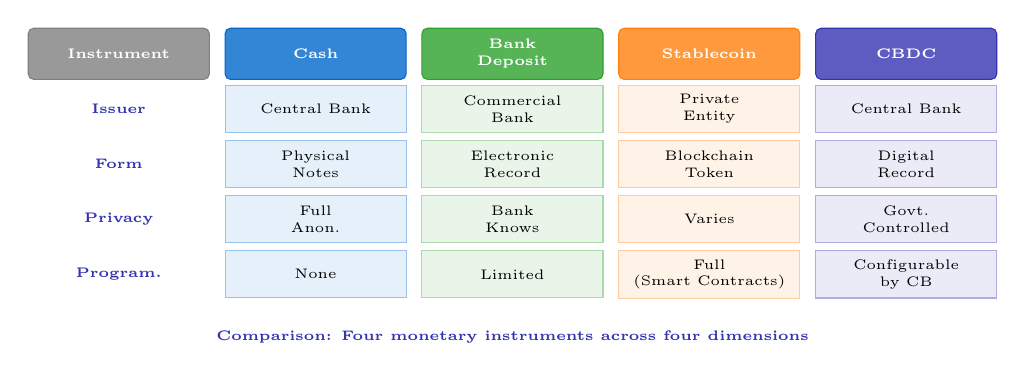
\begin{tikzpicture}[
  lhdr/.style={font=\tiny\bfseries, text=mlpurple, align=center}
]
  %% Column headers
  \node[draw=mlgray, fill=mlgray!80, rounded corners=2pt, minimum width=2.3cm, minimum height=0.65cm, align=center, font=\tiny\bfseries, text=white]   at (1.5,5.1) {Instrument};
  \node[draw=mlblue, fill=mlblue!80, rounded corners=2pt, minimum width=2.3cm, minimum height=0.65cm, align=center, font=\tiny\bfseries, text=white]   at (4.0,5.1) {Cash};
  \node[draw=mlgreen, fill=mlgreen!80, rounded corners=2pt, minimum width=2.3cm, minimum height=0.65cm, align=center, font=\tiny\bfseries, text=white]  at (6.5,5.1) {Bank\\Deposit};
  \node[draw=mlorange, fill=mlorange!80, rounded corners=2pt, minimum width=2.3cm, minimum height=0.65cm, align=center, font=\tiny\bfseries, text=white] at (9.0,5.1) {Stablecoin};
  \node[draw=mlpurple, fill=mlpurple!80, rounded corners=2pt, minimum width=2.3cm, minimum height=0.65cm, align=center, font=\tiny\bfseries, text=white] at (11.5,5.1) {CBDC};

  %% Row: Issuer
  \node[lhdr=mlgray]  at (1.5,4.4) {Issuer};
  \node[draw=mlblue!40, fill=mlblue!10, minimum width=2.3cm, minimum height=0.6cm, align=center, font=\tiny]   at (4.0,4.4) {Central Bank};
  \node[draw=mlgreen!40, fill=mlgreen!10, minimum width=2.3cm, minimum height=0.6cm, align=center, font=\tiny]  at (6.5,4.4) {Commercial\\Bank};
  \node[draw=mlorange!40, fill=mlorange!10, minimum width=2.3cm, minimum height=0.6cm, align=center, font=\tiny] at (9.0,4.4) {Private\\Entity};
  \node[draw=mlpurple!40, fill=mlpurple!10, minimum width=2.3cm, minimum height=0.6cm, align=center, font=\tiny] at (11.5,4.4) {Central Bank};

  %% Row: Form
  \node[lhdr=mlgray]  at (1.5,3.7) {Form};
  \node[draw=mlblue!40, fill=mlblue!10, minimum width=2.3cm, minimum height=0.6cm, align=center, font=\tiny]   at (4.0,3.7) {Physical\\Notes};
  \node[draw=mlgreen!40, fill=mlgreen!10, minimum width=2.3cm, minimum height=0.6cm, align=center, font=\tiny]  at (6.5,3.7) {Electronic\\Record};
  \node[draw=mlorange!40, fill=mlorange!10, minimum width=2.3cm, minimum height=0.6cm, align=center, font=\tiny] at (9.0,3.7) {Blockchain\\Token};
  \node[draw=mlpurple!40, fill=mlpurple!10, minimum width=2.3cm, minimum height=0.6cm, align=center, font=\tiny] at (11.5,3.7) {Digital\\Record};

  %% Row: Privacy
  \node[lhdr=mlgray]  at (1.5,3.0) {Privacy};
  \node[draw=mlblue!40, fill=mlblue!10, minimum width=2.3cm, minimum height=0.6cm, align=center, font=\tiny]   at (4.0,3.0) {Full\\Anon.};
  \node[draw=mlgreen!40, fill=mlgreen!10, minimum width=2.3cm, minimum height=0.6cm, align=center, font=\tiny]  at (6.5,3.0) {Bank\\Knows};
  \node[draw=mlorange!40, fill=mlorange!10, minimum width=2.3cm, minimum height=0.6cm, align=center, font=\tiny] at (9.0,3.0) {Varies};
  \node[draw=mlpurple!40, fill=mlpurple!10, minimum width=2.3cm, minimum height=0.6cm, align=center, font=\tiny] at (11.5,3.0) {Govt.\\Controlled};

  %% Row: Programmable
  \node[lhdr=mlgray]   at (1.5,2.3) {Program.};
  \node[draw=mlblue!40, fill=mlblue!10, minimum width=2.3cm, minimum height=0.6cm, align=center, font=\tiny]    at (4.0,2.3) {None};
  \node[draw=mlgreen!40, fill=mlgreen!10, minimum width=2.3cm, minimum height=0.6cm, align=center, font=\tiny]   at (6.5,2.3) {Limited};
  \node[draw=mlorange!40, fill=mlorange!10, minimum width=2.3cm, minimum height=0.6cm, align=center, font=\tiny]  at (9.0,2.3) {Full\\(Smart Contracts)};
  \node[draw=mlpurple!40, fill=mlpurple!10, minimum width=2.3cm, minimum height=0.6cm, align=center, font=\tiny]  at (11.5,2.3) {Configurable\\by CB};

  \node[font=\tiny\bfseries, text=mlpurple, align=center] at (6.5,1.5) {Comparison: Four monetary instruments across four dimensions};
\end{tikzpicture}
\end{columns}
\bottomnote{BIS definition: CBDC is a digital form of CB money, different from existing reserves | IMF: 100+ countries in various stages of CBDC exploration | First live CBDC: Bahamas Sand Dollar, Oct 2020}
\end{frame}

% Frame 41: CBDC Motivation
\begin{frame}{Why Are Central Banks Pursuing CBDCs?}
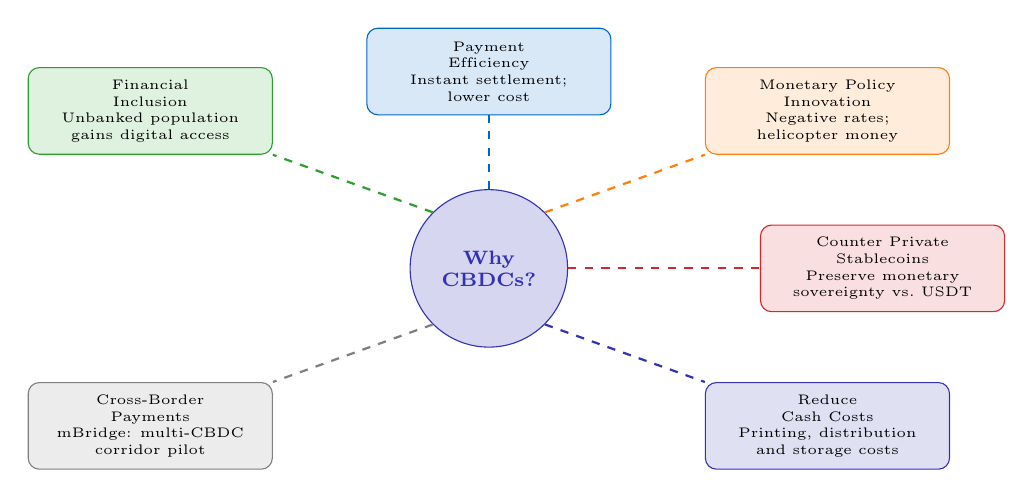
\begin{tikzpicture}[
  hub/.style={draw=mlpurple, fill=mlpurple!20, circle, minimum size=2.0cm, align=center, font=\scriptsize\bfseries, text=mlpurple}
]
  %% Centre hub
  \node[hub] (ctr) at (5.5,3.0) {Why\\CBDCs?};

  %% Spoke 1: Financial Inclusion (top-left)
  \node[draw=mlgreen, fill=mlgreen!15, rounded corners=4pt, minimum width=3.1cm, minimum height=1.1cm, align=center, font=\tiny] (fi) at (1.2,5.0) {Financial\\Inclusion\\Unbanked population\\gains digital access};
  \draw[thick, mlgreen, dashed] (ctr.north west) -- (fi.south east);

  %% Spoke 2: Payment Efficiency (top)
  \node[draw=mlblue, fill=mlblue!15, rounded corners=4pt, minimum width=3.1cm, minimum height=1.1cm, align=center, font=\tiny] (pe) at (5.5,5.5) {Payment\\Efficiency\\Instant settlement;\\lower cost};
  \draw[thick, mlblue, dashed] (ctr.north) -- (pe.south);

  %% Spoke 3: Monetary Policy Innovation (top-right)
  \node[draw=mlorange, fill=mlorange!15, rounded corners=4pt, minimum width=3.1cm, minimum height=1.1cm, align=center, font=\tiny] (mp) at (9.8,5.0) {Monetary Policy\\Innovation\\Negative rates;\\helicopter money};
  \draw[thick, mlorange, dashed] (ctr.north east) -- (mp.south west);

  %% Spoke 4: Counter Private Stablecoins (right)
  \node[draw=mlred, fill=mlred!15, rounded corners=4pt, minimum width=3.1cm, minimum height=1.1cm, align=center, font=\tiny] (cp) at (10.5,3.0) {Counter Private\\Stablecoins\\Preserve monetary\\sovereignty vs.\ USDT};
  \draw[thick, mlred, dashed] (ctr.east) -- (cp.west);

  %% Spoke 5: Reduce Cash Costs (bottom-right)
  \node[draw=mlpurple, fill=mlpurple!15, rounded corners=4pt, minimum width=3.1cm, minimum height=1.1cm, align=center, font=\tiny] (rc) at (9.8,1.0) {Reduce\\Cash Costs\\Printing, distribution\\and storage costs};
  \draw[thick, mlpurple, dashed] (ctr.south east) -- (rc.north west);

  %% Spoke 6: Cross-Border Payments (bottom-left)
  \node[draw=mlgray, fill=mlgray!15, rounded corners=4pt, minimum width=3.1cm, minimum height=1.1cm, align=center, font=\tiny] (cb) at (1.2,1.0) {Cross-Border\\Payments\\mBridge: multi-CBDC\\corridor pilot};
  \draw[thick, mlgray, dashed] (ctr.south west) -- (cb.north east);
\end{tikzpicture}
\bottomnote{BIS survey 2023: 93\% of central banks exploring CBDCs | mBridge: BIS Innovation Hub multi-CBDC platform | Sweden Riksbank: e-Krona pilot since 2020; cash use $<$10\% of transactions | ECB Digital Euro consultation: 6,500+ responses}
\end{frame}

% Frame 42: Wholesale vs Retail CBDC
\begin{frame}{Wholesale vs.\ Retail CBDC}
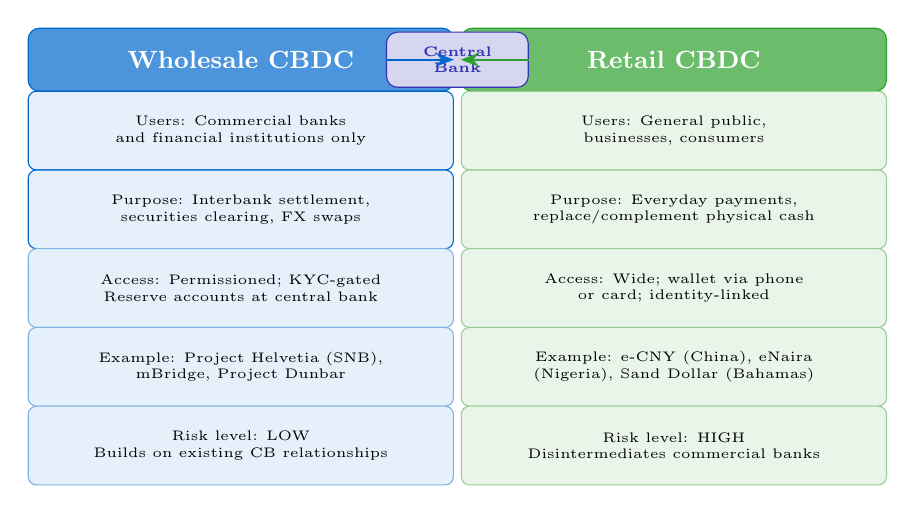
\begin{tikzpicture}
  %% Wholesale panel (left)
  \node[draw=mlblue, fill=mlblue!70, rounded corners=4pt, minimum width=5.4cm, minimum height=0.8cm, align=center, font=\small\bfseries, text=white] (wh) at (3.0,5.5) {Wholesale CBDC};
  \node[draw=mlblue, fill=mlblue!10, rounded corners=3pt, minimum width=5.4cm, minimum height=1.0cm, align=center, font=\tiny] at (3.0,4.6) {Users: Commercial banks\\and financial institutions only};
  \node[draw=mlblue, fill=mlblue!10, rounded corners=3pt, minimum width=5.4cm, minimum height=1.0cm, align=center, font=\tiny] at (3.0,3.6) {Purpose: Interbank settlement,\\securities clearing, FX swaps};
  \node[draw=mlblue!50, fill=mlblue!10, rounded corners=3pt, minimum width=5.4cm, minimum height=1.0cm, align=center, font=\tiny] at (3.0,2.6) {Access: Permissioned; KYC-gated\\Reserve accounts at central bank};
  \node[draw=mlblue!50, fill=mlblue!10, rounded corners=3pt, minimum width=5.4cm, minimum height=1.0cm, align=center, font=\tiny] at (3.0,1.6) {Example: Project Helvetia (SNB),\\mBridge, Project Dunbar};
  \node[draw=mlblue!50, fill=mlblue!10, rounded corners=3pt, minimum width=5.4cm, minimum height=1.0cm, align=center, font=\tiny] at (3.0,0.6) {Risk level: LOW\\Builds on existing CB relationships};

  %% Retail panel (right)
  \node[draw=mlgreen, fill=mlgreen!70, rounded corners=4pt, minimum width=5.4cm, minimum height=0.8cm, align=center, font=\small\bfseries, text=white] (rt) at (8.5,5.5) {Retail CBDC};
  \node[draw=mlgreen!50, fill=mlgreen!10, rounded corners=3pt, minimum width=5.4cm, minimum height=1.0cm, align=center, font=\tiny] at (8.5,4.6) {Users: General public,\\businesses, consumers};
  \node[draw=mlgreen!50, fill=mlgreen!10, rounded corners=3pt, minimum width=5.4cm, minimum height=1.0cm, align=center, font=\tiny] at (8.5,3.6) {Purpose: Everyday payments,\\replace/complement physical cash};
  \node[draw=mlgreen!50, fill=mlgreen!10, rounded corners=3pt, minimum width=5.4cm, minimum height=1.0cm, align=center, font=\tiny] at (8.5,2.6) {Access: Wide; wallet via phone\\or card; identity-linked};
  \node[draw=mlgreen!50, fill=mlgreen!10, rounded corners=3pt, minimum width=5.4cm, minimum height=1.0cm, align=center, font=\tiny] at (8.5,1.6) {Example: e-CNY (China), eNaira\\(Nigeria), Sand Dollar (Bahamas)};
  \node[draw=mlgreen!50, fill=mlgreen!10, rounded corners=3pt, minimum width=5.4cm, minimum height=1.0cm, align=center, font=\tiny] at (8.5,0.6) {Risk level: HIGH\\Disintermediates commercial banks};

  %% Central Bank node
  \node[draw=mlpurple, fill=mlpurple!20, rounded corners=4pt, minimum width=1.8cm, minimum height=0.7cm, align=center, font=\tiny\bfseries, text=mlpurple] (cb) at (5.75,5.5) {Central\\Bank};
  \draw[-{Stealth}, thick, mlblue]  (cb.west)  -- (wh.east);
  \draw[-{Stealth}, thick, mlgreen] (cb.east)  -- (rt.west);
\end{tikzpicture}
\bottomnote{Most early CBDCs are retail-focused | Wholesale CBDCs less disruptive to banking sector | mBridge: China, UAE, Thailand, HK multi-currency wholesale corridor | BIS: both types possible in parallel}
\end{frame}

% Frame 43: CBDC Architecture Models
\begin{frame}{CBDC Architecture Models}
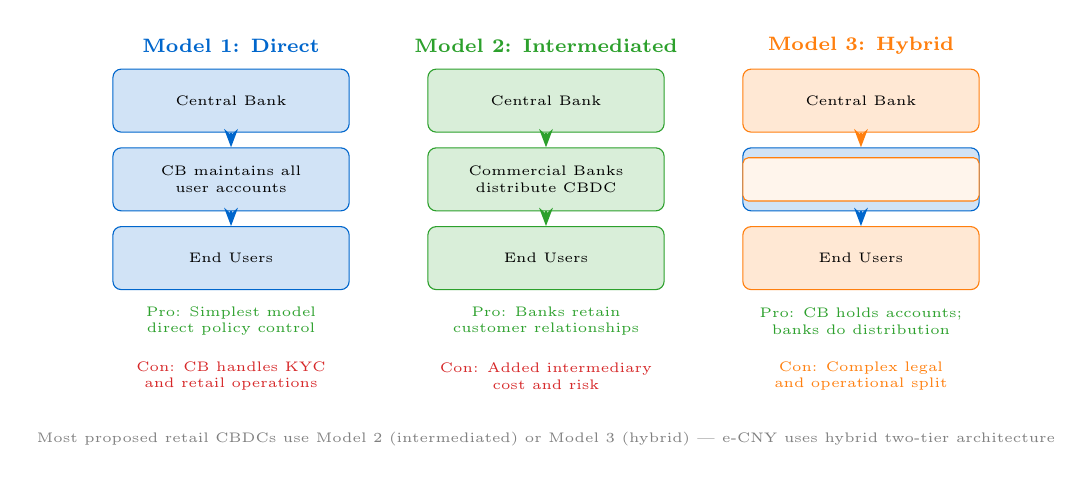
\begin{tikzpicture}
  %% Model 1: Direct
  \node[font=\scriptsize\bfseries, text=mlblue] at (1.8,5.7) {Model 1: Direct};
  \node[draw=mlblue, fill=mlblue!18, rounded corners=3pt, minimum width=3.0cm, minimum height=0.8cm, align=center, font=\tiny] (d_cb)  at (1.8,5.0) {Central Bank};
  \node[draw=mlblue, fill=mlblue!18, rounded corners=3pt, minimum width=3.0cm, minimum height=0.8cm, align=center, font=\tiny] (d_acc) at (1.8,4.0) {CB maintains all\\user accounts};
  \node[draw=mlblue, fill=mlblue!18, rounded corners=3pt, minimum width=3.0cm, minimum height=0.8cm, align=center, font=\tiny] (d_usr) at (1.8,3.0) {End Users};
  \draw[-{Stealth}, thick, mlblue] (d_cb.south)  -- (d_acc.north);
  \draw[-{Stealth}, thick, mlblue] (d_acc.south) -- (d_usr.north);
  \node[font=\tiny, text=mlgreen, align=center] at (1.8,2.2) {Pro: Simplest model\\direct policy control};
  \node[font=\tiny, text=mlred, align=center]   at (1.8,1.5) {Con: CB handles KYC\\and retail operations};

  %% Model 2: Intermediated
  \node[font=\scriptsize\bfseries, text=mlgreen] at (5.8,5.7) {Model 2: Intermediated};
  \node[draw=mlgreen, fill=mlgreen!18, rounded corners=3pt, minimum width=3.0cm, minimum height=0.8cm, align=center, font=\tiny] (i_cb)  at (5.8,5.0) {Central Bank};
  \node[draw=mlgreen, fill=mlgreen!18, rounded corners=3pt, minimum width=3.0cm, minimum height=0.8cm, align=center, font=\tiny] (i_bk)  at (5.8,4.0) {Commercial Banks\\distribute CBDC};
  \node[draw=mlgreen, fill=mlgreen!18, rounded corners=3pt, minimum width=3.0cm, minimum height=0.8cm, align=center, font=\tiny] (i_usr) at (5.8,3.0) {End Users};
  \draw[-{Stealth}, thick, mlgreen] (i_cb.south)  -- (i_bk.north);
  \draw[-{Stealth}, thick, mlgreen] (i_bk.south)  -- (i_usr.north);
  \node[font=\tiny, text=mlgreen, align=center] at (5.8,2.2) {Pro: Banks retain\\customer relationships};
  \node[font=\tiny, text=mlred, align=center]   at (5.8,1.5) {Con: Added intermediary\\cost and risk};

  %% Model 3: Hybrid
  \node[font=\scriptsize\bfseries, text=mlorange] at (9.8,5.7) {Model 3: Hybrid};
  \node[draw=mlorange, fill=mlorange!18, rounded corners=3pt, minimum width=3.0cm, minimum height=0.8cm, align=center, font=\tiny] (h_cb)  at (9.8,5.0) {Central Bank};
  \node[draw=mlblue, fill=mlblue!18, rounded corners=3pt, minimum width=3.0cm, minimum height=0.8cm, align=center, font=\tiny]   (h_bk)  at (9.8,4.0) {Banks: front-end\\payments processing};
  \node[draw=mlorange, fill=mlorange!18, rounded corners=3pt, minimum width=3.0cm, minimum height=0.8cm, align=center, font=\tiny] (h_usr) at (9.8,3.0) {End Users};
  \draw[-{Stealth}, thick, mlorange] (h_cb.south)  -- (h_bk.north);
  \draw[-{Stealth}, thick, mlblue]   (h_bk.south)  -- (h_usr.north);
  \node[draw=mlorange, fill=mlorange!8, rounded corners=2pt, minimum width=3.0cm, minimum height=0.55cm, align=center, font=\tiny] at (9.8,4.0) {};
  \node[font=\tiny, text=mlgreen, align=center]  at (9.8,2.2) {Pro: CB holds accounts;\\banks do distribution};
  \node[font=\tiny, text=mlorange, align=center] at (9.8,1.5) {Con: Complex legal\\and operational split};

  \node[font=\tiny, text=mlgray, align=center] at (5.8,0.7) {Most proposed retail CBDCs use Model 2 (intermediated) or Model 3 (hybrid) | e-CNY uses hybrid two-tier architecture};
\end{tikzpicture}
\bottomnote{IMF: 60\% of CBDC pilots use two-tier (intermediated) model | Digital Euro: hybrid model proposed | e-CNY: hybrid with PBOC at top, state banks distributing | Direct model: used in Eastern Caribbean (DCash)}
\end{frame}

% Frame 44: Account-Based vs Token-Based [FRAGILE] -- CODE FRAME 3
\begin{frame}[fragile]{Account-Based vs Token-Based}
\begin{columns}[T]
\column{0.50\textwidth}
\begin{lstlisting}[language=Solidity, caption={Account-Based CBDC Interface}]
// Account-based CBDC model
interface IAccountCBDC {
    function balanceOf(address account)
        external view returns (uint256);
    function transfer(
        address to, uint256 amount
    ) external returns (bool);
    function freeze(address account)
        external; // regulatory
    function setSpendingLimit(
        address account, uint256 limit
    ) external;
}
\end{lstlisting}
\vspace{2mm}
\begin{alertblock}{Design Choice Impact}
\scriptsize Account-based: identity is primary --- you prove who you are. Token-based: possession is primary --- you prove you have the token. This determines privacy, offline capability, and programmability.
\end{alertblock}
\column{0.50\textwidth}
\begin{block}{Account-Based}
\begin{itemize}\setlength{\itemsep}{2pt}
  \item \textbf{Identity-linked:} Balance tied to verified identity; KYC enforced at account opening
  \item \textbf{Regulatory tools:} \texttt{freeze()} and \texttt{setSpendingLimit()} enable direct control
  \item \textbf{Traceability:} Full transaction history visible to issuer; AML-compliant
  \item \textbf{Offline:} Difficult; requires identity verification at every transfer
\end{itemize}
\end{block}
\vspace{2mm}
\begin{block}{Token-Based}
\begin{itemize}\setlength{\itemsep}{2pt}
  \item \textbf{Possession-based:} Valid token = valid payment; like digital banknote
  \item \textbf{Privacy:} Bearer instrument; sender/receiver can be pseudonymous
  \item \textbf{Offline:} Possible via secure hardware element (TEE/SE chips)
  \item \textbf{Double-spend:} Requires cryptographic prevention (blind signatures, hardware)
\end{itemize}
\end{block}
\end{columns}
\bottomnote{e-CNY: account-based with tiered anonymity | Digital Euro: exploring hybrid with low-value offline token capability | BIS working paper 976: privacy-preserving CBDC via zero-knowledge proofs | Most designs: account-based for AML compliance}
\end{frame}

% Frame 45: Global CBDC Landscape
\begin{frame}{Global CBDC Landscape}
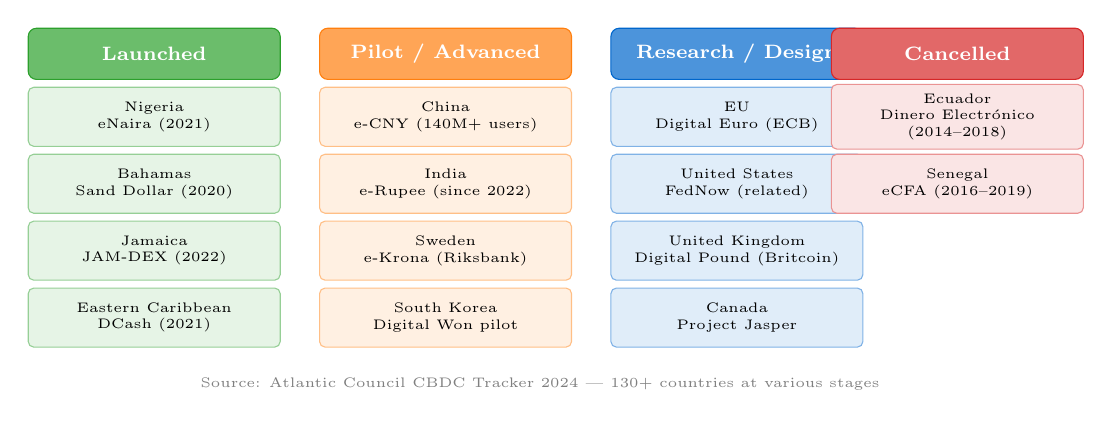
\begin{tikzpicture}
  %% Launched column
  \node[draw=mlgreen, fill=mlgreen!70, rounded corners=3pt, minimum width=3.2cm, minimum height=0.65cm, align=center, font=\scriptsize\bfseries, text=white]  at (1.8,5.5) {Launched};
  \node[draw=mlgreen!50, fill=mlgreen!12, rounded corners=2pt, minimum width=3.2cm, minimum height=0.75cm, align=center, font=\tiny]  at (1.8,4.7) {Nigeria\\eNaira (2021)};
  \node[draw=mlgreen!50, fill=mlgreen!12, rounded corners=2pt, minimum width=3.2cm, minimum height=0.75cm, align=center, font=\tiny]  at (1.8,3.85) {Bahamas\\Sand Dollar (2020)};
  \node[draw=mlgreen!50, fill=mlgreen!12, rounded corners=2pt, minimum width=3.2cm, minimum height=0.75cm, align=center, font=\tiny]  at (1.8,3.0) {Jamaica\\JAM-DEX (2022)};
  \node[draw=mlgreen!50, fill=mlgreen!12, rounded corners=2pt, minimum width=3.2cm, minimum height=0.75cm, align=center, font=\tiny]  at (1.8,2.15) {Eastern Caribbean\\DCash (2021)};

  %% Pilot column
  \node[draw=mlorange, fill=mlorange!70, rounded corners=3pt, minimum width=3.2cm, minimum height=0.65cm, align=center, font=\scriptsize\bfseries, text=white] at (5.5,5.5) {Pilot / Advanced};
  \node[draw=mlorange!50, fill=mlorange!12, rounded corners=2pt, minimum width=3.2cm, minimum height=0.75cm, align=center, font=\tiny] at (5.5,4.7) {China\\e-CNY (140M+ users)};
  \node[draw=mlorange!50, fill=mlorange!12, rounded corners=2pt, minimum width=3.2cm, minimum height=0.75cm, align=center, font=\tiny] at (5.5,3.85) {India\\e-Rupee (since 2022)};
  \node[draw=mlorange!50, fill=mlorange!12, rounded corners=2pt, minimum width=3.2cm, minimum height=0.75cm, align=center, font=\tiny] at (5.5,3.0) {Sweden\\e-Krona (Riksbank)};
  \node[draw=mlorange!50, fill=mlorange!12, rounded corners=2pt, minimum width=3.2cm, minimum height=0.75cm, align=center, font=\tiny] at (5.5,2.15) {South Korea\\Digital Won pilot};

  %% Research column
  \node[draw=mlblue, fill=mlblue!70, rounded corners=3pt, minimum width=3.2cm, minimum height=0.65cm, align=center, font=\scriptsize\bfseries, text=white]   at (9.2,5.5) {Research / Design};
  \node[draw=mlblue!50, fill=mlblue!12, rounded corners=2pt, minimum width=3.2cm, minimum height=0.75cm, align=center, font=\tiny]   at (9.2,4.7) {EU\\Digital Euro (ECB)};
  \node[draw=mlblue!50, fill=mlblue!12, rounded corners=2pt, minimum width=3.2cm, minimum height=0.75cm, align=center, font=\tiny]   at (9.2,3.85) {United States\\FedNow (related)};
  \node[draw=mlblue!50, fill=mlblue!12, rounded corners=2pt, minimum width=3.2cm, minimum height=0.75cm, align=center, font=\tiny]   at (9.2,3.0) {United Kingdom\\Digital Pound (Britcoin)};
  \node[draw=mlblue!50, fill=mlblue!12, rounded corners=2pt, minimum width=3.2cm, minimum height=0.75cm, align=center, font=\tiny]   at (9.2,2.15) {Canada\\Project Jasper};

  %% Cancelled column
  \node[draw=mlred, fill=mlred!70, rounded corners=3pt, minimum width=3.2cm, minimum height=0.65cm, align=center, font=\scriptsize\bfseries, text=white]    at (12.0,5.5) {Cancelled};
  \node[draw=mlred!50, fill=mlred!12, rounded corners=2pt, minimum width=3.2cm, minimum height=0.75cm, align=center, font=\tiny]    at (12.0,4.7) {Ecuador\\Dinero Electr\'{o}nico\\(2014--2018)};
  \node[draw=mlred!50, fill=mlred!12, rounded corners=2pt, minimum width=3.2cm, minimum height=0.75cm, align=center, font=\tiny]    at (12.0,3.85) {Senegal\\eCFA (2016--2019)};

  \node[font=\tiny, text=mlgray, align=center] at (6.7,1.3) {Source: Atlantic Council CBDC Tracker 2024 | 130+ countries at various stages};
\end{tikzpicture}
\bottomnote{Atlantic Council CBDC Tracker: 130 countries in some stage of CBDC | G7: all have active research programs | BIS mBridge: 26 observing members | eNaira adoption challenged by low uptake; only 0.5\% of Nigerians used it by 2023}
\end{frame}

% Frame 46: China's Digital Yuan (e-CNY)
\begin{frame}{China's Digital Yuan: e-CNY}
\begin{columns}[T]
\column{0.44\textwidth}
\begin{block}{Key Facts}
\begin{itemize}\setlength{\itemsep}{2pt}
  \item \textbf{Issuer:} People's Bank of China (PBOC)
  \item \textbf{Launch:} Pilot since 2019; expanded to 26 cities
  \item \textbf{Users:} 260M+ registered wallets (2023)
  \item \textbf{Transactions:} \$250B+ in pilot transactions
  \item \textbf{Technology:} Proprietary; not on public blockchain
  \item \textbf{Tiers:} Four wallet tiers by ID verification level
  \item \textbf{Anonymity:} Managed: PBOC sees all, but limited visibility for merchants
\end{itemize}
\end{block}
\vspace{2mm}
\begin{block}{Strategic Objectives}
\begin{itemize}\setlength{\itemsep}{2pt}
  \item Reduce dependence on USD in international trade
  \item Counter Alipay/WeChat Pay duopoly
  \item Enable programmable fiscal stimulus (expiry-dated vouchers)
  \item Lay groundwork for cross-border CNY settlement
\end{itemize}
\end{block}
\column{0.56\textwidth}
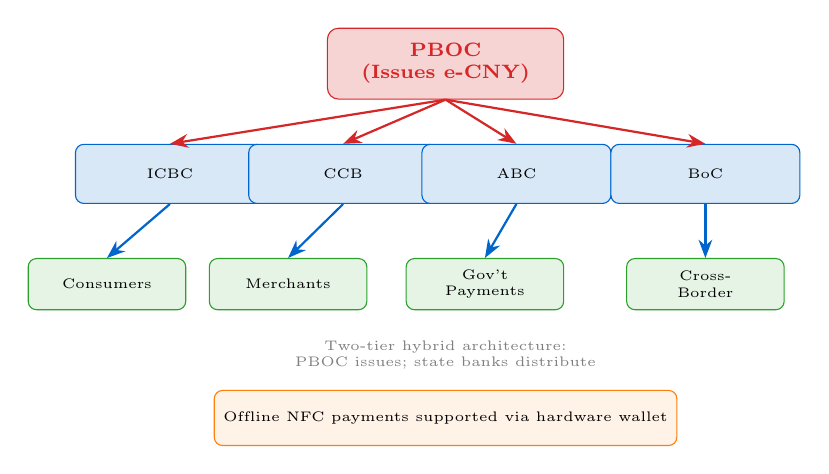
\begin{tikzpicture}[
  node_cb/.style={draw=mlred, fill=mlred!20, rounded corners=4pt, minimum width=3.0cm, minimum height=0.9cm, align=center, font=\scriptsize\bfseries, text=mlred},
  node_bk/.style={draw=mlblue, fill=mlblue!15, rounded corners=3pt, minimum width=2.4cm, minimum height=0.75cm, align=center, font=\tiny},
  node_usr/.style={draw=mlgreen, fill=mlgreen!12, rounded corners=3pt, minimum width=2.0cm, minimum height=0.65cm, align=center, font=\tiny}
]
  %% PBOC at top
  \node[node_cb] (pboc) at (5.5,5.2) {PBOC\\(Issues e-CNY)};

  %% Tier 1 banks
  \node[node_bk] (icbc) at (2.0,3.8) {ICBC};
  \node[node_bk] (ccb)  at (4.2,3.8) {CCB};
  \node[node_bk] (abc)  at (6.4,3.8) {ABC};
  \node[node_bk] (boc)  at (8.8,3.8) {BoC};

  \draw[-{Stealth}, thick, mlred] (pboc.south) -- (icbc.north);
  \draw[-{Stealth}, thick, mlred] (pboc.south) -- (ccb.north);
  \draw[-{Stealth}, thick, mlred] (pboc.south) -- (abc.north);
  \draw[-{Stealth}, thick, mlred] (pboc.south) -- (boc.north);

  %% Users / Merchants
  \node[node_usr] (u1) at (1.2,2.4) {Consumers};
  \node[node_usr] (u2) at (3.5,2.4) {Merchants};
  \node[node_usr] (u3) at (6.0,2.4) {Gov't\\Payments};
  \node[node_usr] (u4) at (8.8,2.4) {Cross-\\Border};

  \draw[-{Stealth}, thick, mlblue] (icbc.south) -- (u1.north);
  \draw[-{Stealth}, thick, mlblue] (ccb.south)  -- (u2.north);
  \draw[-{Stealth}, thick, mlblue] (abc.south)  -- (u3.north);
  \draw[-{Stealth}, thick, mlblue] (boc.south)  -- (u4.north);

  %% Label
  \node[font=\tiny, text=mlgray, align=center] at (5.5,1.5) {Two-tier hybrid architecture:\\PBOC issues; state banks distribute};

  %% Offline capability note
  \node[draw=mlorange, fill=mlorange!10, rounded corners=3pt, minimum width=5.0cm, minimum height=0.7cm, align=center, font=\tiny] at (5.5,0.7) {Offline NFC payments supported via hardware wallet};
\end{tikzpicture}
\end{columns}
\bottomnote{e-CNY used at Beijing 2022 Olympics | PBOC goal: domestic cash replacement + cross-border USD alternative | mBridge connects e-CNY with HK, UAE, Thailand CBDCs | Privacy concern: controlled anonymity --- PBOC retains full oversight}
\end{frame}

% Frame 47: Privacy in CBDCs
\begin{frame}{Privacy in CBDCs: A Spectrum}
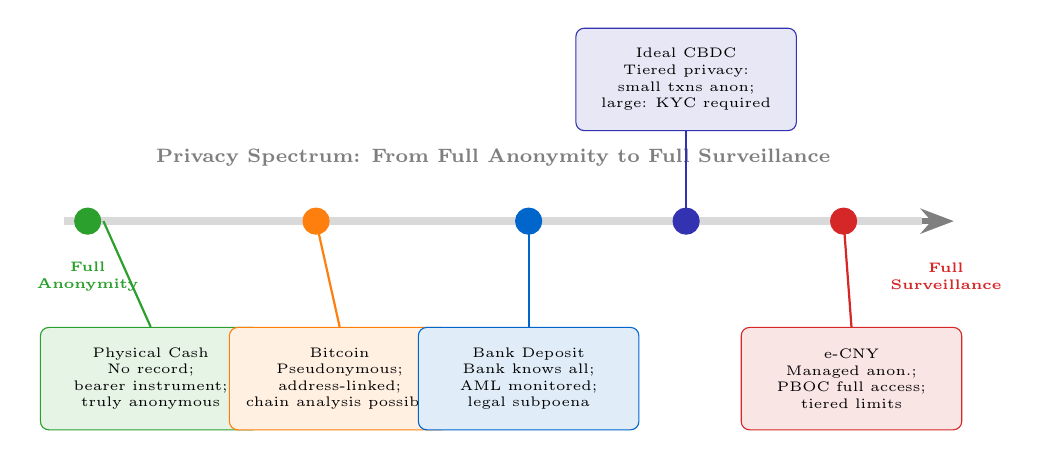
\begin{tikzpicture}
  %% Main spectrum axis
  \draw[line width=3pt, mlgray!30] (0.3,3.5) -- (11.2,3.5);
  \draw[-{Stealth}, line width=2pt, mlgray] (11.2,3.5) -- (11.6,3.5);
  \node[font=\scriptsize\bfseries, text=mlgray, align=center] at (5.75,4.3) {Privacy Spectrum: From Full Anonymity to Full Surveillance};

  %% Left pole: Full anonymity
  \node[font=\tiny\bfseries, text=mlgreen, align=center] at (0.6,2.8) {Full\\Anonymity};
  \node[draw=mlgreen, fill=mlgreen, circle, minimum size=0.3cm] at (0.6,3.5) {};

  %% Right pole: Full surveillance
  \node[font=\tiny\bfseries, text=mlred, align=center] at (11.5,2.8) {Full\\Surveillance};

  %% Cash
  \node[draw=mlgreen, fill=mlgreen!12, rounded corners=3pt, minimum width=2.8cm, minimum height=1.3cm, align=center, font=\tiny] (cash) at (1.4,1.5) {Physical Cash\\No record;\\bearer instrument;\\truly anonymous};
  \draw[thick, mlgreen] (cash.north) -- (0.8,3.5);

  %% Bitcoin
  \node[draw=mlorange, fill=mlorange!12, rounded corners=3pt, minimum width=2.8cm, minimum height=1.3cm, align=center, font=\tiny] (btc) at (3.8,1.5) {Bitcoin\\Pseudonymous;\\address-linked;\\chain analysis possible};
  \draw[thick, mlorange] (btc.north) -- (3.5,3.5);
  \node[draw=mlorange, fill=mlorange, circle, minimum size=0.3cm] at (3.5,3.5) {};

  %% Bank deposit
  \node[draw=mlblue, fill=mlblue!12, rounded corners=3pt, minimum width=2.8cm, minimum height=1.3cm, align=center, font=\tiny] (bank) at (6.2,1.5) {Bank Deposit\\Bank knows all;\\AML monitored;\\legal subpoena};
  \draw[thick, mlblue] (bank.north) -- (6.2,3.5);
  \node[draw=mlblue, fill=mlblue, circle, minimum size=0.3cm] at (6.2,3.5) {};

  %% Ideal CBDC
  \node[draw=mlpurple, fill=mlpurple!12, rounded corners=3pt, minimum width=2.8cm, minimum height=1.3cm, align=center, font=\tiny] (cbdc_i) at (8.2,5.3) {Ideal CBDC\\Tiered privacy:\\small txns anon;\\large: KYC required};
  \draw[thick, mlpurple] (cbdc_i.south) -- (8.2,3.5);
  \node[draw=mlpurple, fill=mlpurple, circle, minimum size=0.3cm] at (8.2,3.5) {};

  %% e-CNY
  \node[draw=mlred, fill=mlred!12, rounded corners=3pt, minimum width=2.8cm, minimum height=1.3cm, align=center, font=\tiny] (ecny) at (10.3,1.5) {e-CNY\\Managed anon.;\\PBOC full access;\\tiered limits};
  \draw[thick, mlred] (ecny.north) -- (10.2,3.5);
  \node[draw=mlred, fill=mlred, circle, minimum size=0.3cm] at (10.2,3.5) {};
\end{tikzpicture}
\bottomnote{ECB Digital Euro: privacy by design, offline payments without traceability for small amounts | BIS: tiered privacy model most likely for retail CBDCs | ZKP-based approaches (e.g., MIT Hamilton project) can provide privacy with AML compliance | Key tension: financial surveillance vs.\ civil liberties}
\end{frame}

% Frame 48: Section 4 Summary
\begin{frame}{Section 4 Summary}
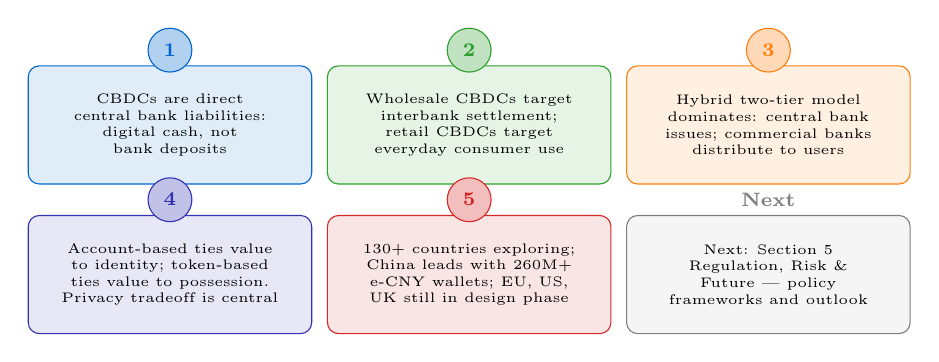
\begin{tikzpicture}
  \node[draw=mlblue, fill=mlblue!12, rounded corners=4pt, minimum width=3.6cm, minimum height=1.5cm, align=center, font=\tiny] (k1) at (1.9,3.2) {CBDCs are direct\\central bank liabilities:\\digital cash, not\\bank deposits};
  \node[circle, draw=mlblue, fill=mlblue!30, minimum size=0.55cm, font=\scriptsize\bfseries, text=mlblue] at (1.9,4.15) {1};

  \node[draw=mlgreen, fill=mlgreen!12, rounded corners=4pt, minimum width=3.6cm, minimum height=1.5cm, align=center, font=\tiny] (k2) at (5.7,3.2) {Wholesale CBDCs target\\interbank settlement;\\retail CBDCs target\\everyday consumer use};
  \node[circle, draw=mlgreen, fill=mlgreen!30, minimum size=0.55cm, font=\scriptsize\bfseries, text=mlgreen] at (5.7,4.15) {2};

  \node[draw=mlorange, fill=mlorange!12, rounded corners=4pt, minimum width=3.6cm, minimum height=1.5cm, align=center, font=\tiny] (k3) at (9.5,3.2) {Hybrid two-tier model\\dominates: central bank\\issues; commercial banks\\distribute to users};
  \node[circle, draw=mlorange, fill=mlorange!30, minimum size=0.55cm, font=\scriptsize\bfseries, text=mlorange] at (9.5,4.15) {3};

  \node[draw=mlpurple, fill=mlpurple!12, rounded corners=4pt, minimum width=3.6cm, minimum height=1.5cm, align=center, font=\tiny] (k4) at (1.9,1.3) {Account-based ties value\\to identity; token-based\\ties value to possession.\\Privacy tradeoff is central};
  \node[circle, draw=mlpurple, fill=mlpurple!30, minimum size=0.55cm, font=\scriptsize\bfseries, text=mlpurple] at (1.9,2.25) {4};

  \node[draw=mlred, fill=mlred!12, rounded corners=4pt, minimum width=3.6cm, minimum height=1.5cm, align=center, font=\tiny] (k5) at (5.7,1.3) {130+ countries exploring;\\China leads with 260M+\\e-CNY wallets; EU, US,\\UK still in design phase};
  \node[circle, draw=mlred, fill=mlred!30, minimum size=0.55cm, font=\scriptsize\bfseries, text=mlred] at (5.7,2.25) {5};

  \node[draw=mlgray, fill=mlgray!8, rounded corners=4pt, minimum width=3.6cm, minimum height=1.5cm, align=center, font=\tiny] (k6) at (9.5,1.3) {Next: Section 5\\Regulation, Risk \&\\Future --- policy\\frameworks and outlook};
  \node[font=\scriptsize\bfseries, text=mlgray] at (9.5,2.25) {Next};
\end{tikzpicture}
\bottomnote{Section 4 complete | 5 key takeaways | CBDCs: state response to private stablecoin growth | Proceed to Section 5: Regulation, Risk \& Future}
\end{frame}

%% ============================================================
%% SECTION 5: REGULATION, RISK & FUTURE
%% ============================================================
\section{Regulation, Risk \& Future}

% Frame 49: Section 5 Divider
\begin{frame}{Section 5: Regulation, Risk \& Future}
\begin{beamercolorbox}[sep=12pt,center,rounded=true,shadow=true]{palette quaternary}
  {\Large\bfseries Section 5: Regulation, Risk \& Future}\\[4pt]
  {\normalsize Regulatory frameworks, systemic risks, and the future of programmable money}
\end{beamercolorbox}

\vspace{4mm}
\begin{columns}[T]
\column{0.55\textwidth}
\begin{block}{What You Will Learn}
\begin{itemize}\setlength{\itemsep}{2pt}
  \item Global regulatory frameworks for stablecoins
  \item Systemic risk categories and interdependencies
  \item Stablecoins as DeFi infrastructure components
  \item Cross-border payment revolution underway
  \item Future convergence of stablecoins and CBDCs
\end{itemize}
\end{block}
\column{0.45\textwidth}
\begin{block}{Frames in This Section}
\begin{itemize}\setlength{\itemsep}{2pt}
  \item Frame 50: Regulatory Landscape
  \item Frame 51: Systemic Risk Analysis
  \item Frame 52: Stablecoins in DeFi (Code)
  \item Frame 53: Cross-Border Payments
  \item Frame 54: Future of Programmable Money
  \item Frame 55: Key Takeaways
\end{itemize}
\end{block}
\end{columns}
\bottomnote{Section 5 of 5 | Frames 49--55 | Regulation accelerating globally post-Terra/LUNA collapse | MiCA: world's first comprehensive crypto asset framework}
\end{frame}

% Frame 50: Regulatory Landscape
\begin{frame}{Global Regulatory Landscape for Stablecoins}
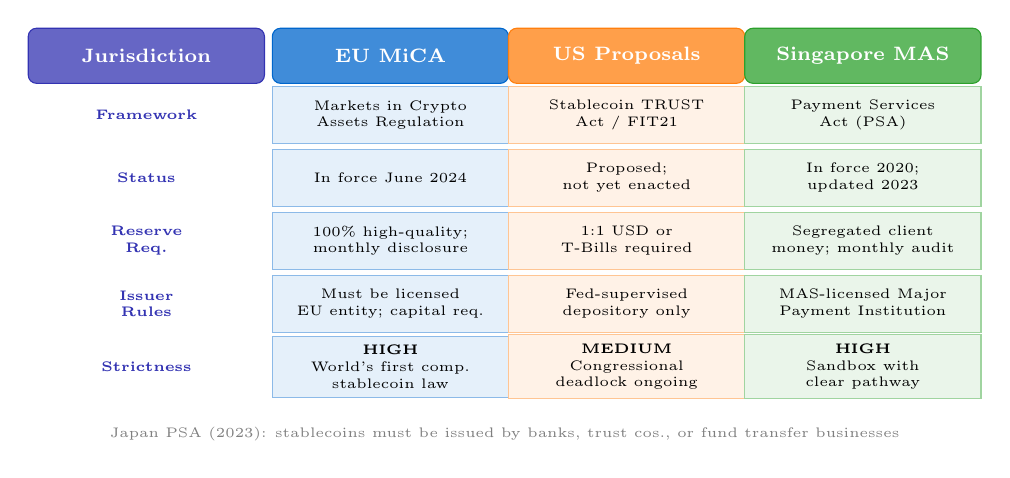
\begin{tikzpicture}[
  lhdr/.style={font=\tiny\bfseries, text=mlpurple, align=center}
]
  %% Column headers
  \node[draw=mlpurple, fill=mlpurple!75, rounded corners=3pt, minimum width=3.0cm, minimum height=0.7cm, align=center, font=\scriptsize\bfseries, text=white]  at (1.8,5.5) {Jurisdiction};
  \node[draw=mlblue,   fill=mlblue!75,   rounded corners=3pt, minimum width=3.0cm, minimum height=0.7cm, align=center, font=\scriptsize\bfseries, text=white]    at (4.9,5.5) {EU MiCA};
  \node[draw=mlorange, fill=mlorange!75, rounded corners=3pt, minimum width=3.0cm, minimum height=0.7cm, align=center, font=\scriptsize\bfseries, text=white]  at (7.9,5.5) {US Proposals};
  \node[draw=mlgreen,  fill=mlgreen!75,  rounded corners=3pt, minimum width=3.0cm, minimum height=0.7cm, align=center, font=\scriptsize\bfseries, text=white]   at (10.9,5.5) {Singapore MAS};

  %% Row: Framework
  \node[lhdr]  at (1.8,4.75) {Framework};
  \node[draw=mlblue!45,   fill=mlblue!10,   minimum width=3.0cm, minimum height=0.72cm, align=center, font=\tiny]   at (4.9,4.75) {Markets in Crypto\\Assets Regulation};
  \node[draw=mlorange!45, fill=mlorange!10, minimum width=3.0cm, minimum height=0.72cm, align=center, font=\tiny] at (7.9,4.75) {Stablecoin TRUST\\Act / FIT21};
  \node[draw=mlgreen!45,  fill=mlgreen!10,  minimum width=3.0cm, minimum height=0.72cm, align=center, font=\tiny]  at (10.9,4.75) {Payment Services\\Act (PSA)};

  %% Row: Status
  \node[lhdr]  at (1.8,3.95) {Status};
  \node[draw=mlblue!45,   fill=mlblue!10,   minimum width=3.0cm, minimum height=0.72cm, align=center, font=\tiny]   at (4.9,3.95) {In force June 2024};
  \node[draw=mlorange!45, fill=mlorange!10, minimum width=3.0cm, minimum height=0.72cm, align=center, font=\tiny] at (7.9,3.95) {Proposed;\\not yet enacted};
  \node[draw=mlgreen!45,  fill=mlgreen!10,  minimum width=3.0cm, minimum height=0.72cm, align=center, font=\tiny]  at (10.9,3.95) {In force 2020;\\updated 2023};

  %% Row: Reserve requirement
  \node[lhdr]  at (1.8,3.15) {Reserve\\Req.};
  \node[draw=mlblue!45,   fill=mlblue!10,   minimum width=3.0cm, minimum height=0.72cm, align=center, font=\tiny]   at (4.9,3.15) {100\% high-quality;\\monthly disclosure};
  \node[draw=mlorange!45, fill=mlorange!10, minimum width=3.0cm, minimum height=0.72cm, align=center, font=\tiny] at (7.9,3.15) {1:1 USD or\\T-Bills required};
  \node[draw=mlgreen!45,  fill=mlgreen!10,  minimum width=3.0cm, minimum height=0.72cm, align=center, font=\tiny]  at (10.9,3.15) {Segregated client\\money; monthly audit};

  %% Row: Issuer
  \node[lhdr]  at (1.8,2.35) {Issuer\\Rules};
  \node[draw=mlblue!45,   fill=mlblue!10,   minimum width=3.0cm, minimum height=0.72cm, align=center, font=\tiny]   at (4.9,2.35) {Must be licensed\\EU entity; capital req.};
  \node[draw=mlorange!45, fill=mlorange!10, minimum width=3.0cm, minimum height=0.72cm, align=center, font=\tiny] at (7.9,2.35) {Fed-supervised\\depository only};
  \node[draw=mlgreen!45,  fill=mlgreen!10,  minimum width=3.0cm, minimum height=0.72cm, align=center, font=\tiny]  at (10.9,2.35) {MAS-licensed Major\\Payment Institution};

  %% Row: Strictness indicator
  \node[lhdr]  at (1.8,1.55) {Strictness};
  \node[draw=mlblue!45,   fill=mlblue!10,   minimum width=3.0cm, minimum height=0.72cm, align=center, font=\tiny]   at (4.9,1.55) {\textbf{HIGH}\\World's first comp.\\stablecoin law};
  \node[draw=mlorange!45, fill=mlorange!10, minimum width=3.0cm, minimum height=0.72cm, align=center, font=\tiny] at (7.9,1.55) {\textbf{MEDIUM}\\Congressional\\deadlock ongoing};
  \node[draw=mlgreen!45,  fill=mlgreen!10,  minimum width=3.0cm, minimum height=0.72cm, align=center, font=\tiny]  at (10.9,1.55) {\textbf{HIGH}\\Sandbox with\\clear pathway};

  \node[font=\tiny, text=mlgray, align=center] at (6.35,0.7) {Japan PSA (2023): stablecoins must be issued by banks, trust cos., or fund transfer businesses};
\end{tikzpicture}
\bottomnote{MiCA: Art.\ 17--49 cover ARTs and EMTs | USDC compliant with MiCA; Tether (USDT) not compliant as of mid-2024 | FSB: Cross-border regulatory coordination framework 2023 | G20: stablecoin regulation a priority since 2021}
\end{frame}

% Frame 51: Systemic Risk Analysis
\begin{frame}{Systemic Risk Analysis}
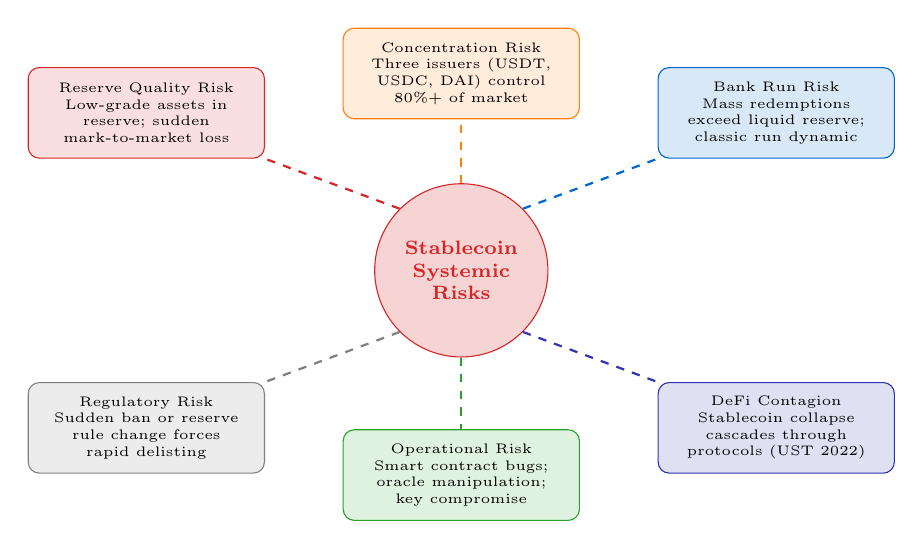
\begin{tikzpicture}[
  ctr/.style={draw=mlred, fill=mlred!20, circle, minimum size=2.2cm, align=center, font=\scriptsize\bfseries, text=mlred}
]
  %% Central risk node
  \node[ctr] (ctr) at (5.5,3.0) {Stablecoin\\Systemic\\Risks};

  %% Risk 1: Reserve quality (top-left)
  \node[draw=mlred, fill=mlred!15, rounded corners=4pt, minimum width=3.0cm, minimum height=1.15cm, align=center, font=\tiny] (rq) at (1.5,5.0) {Reserve Quality Risk\\Low-grade assets in\\reserve; sudden\\mark-to-market loss};
  \draw[thick, dashed, mlred] (ctr.north west) -- (rq.south east);

  %% Risk 2: Concentration (top)
  \node[draw=mlorange, fill=mlorange!15, rounded corners=4pt, minimum width=3.0cm, minimum height=1.15cm, align=center, font=\tiny] (cr) at (5.5,5.5) {Concentration Risk\\Three issuers (USDT,\\USDC, DAI) control\\80\%+ of market};
  \draw[thick, dashed, mlorange] (ctr.north) -- (cr.south);

  %% Risk 3: Bank run (top-right)
  \node[draw=mlblue, fill=mlblue!15, rounded corners=4pt, minimum width=3.0cm, minimum height=1.15cm, align=center, font=\tiny] (br) at (9.5,5.0) {Bank Run Risk\\Mass redemptions\\exceed liquid reserve;\\classic run dynamic};
  \draw[thick, dashed, mlblue] (ctr.north east) -- (br.south west);

  %% Risk 4: Contagion (bottom-right)
  \node[draw=mlpurple, fill=mlpurple!15, rounded corners=4pt, minimum width=3.0cm, minimum height=1.15cm, align=center, font=\tiny] (co) at (9.5,1.0) {DeFi Contagion\\Stablecoin collapse\\cascades through\\protocols (UST 2022)};
  \draw[thick, dashed, mlpurple] (ctr.south east) -- (co.north west);

  %% Risk 5: Regulatory (bottom-left)
  \node[draw=mlgray, fill=mlgray!15, rounded corners=4pt, minimum width=3.0cm, minimum height=1.15cm, align=center, font=\tiny] (re) at (1.5,1.0) {Regulatory Risk\\Sudden ban or reserve\\rule change forces\\rapid delisting};
  \draw[thick, dashed, mlgray] (ctr.south west) -- (re.north east);

  %% Risk 6: Operational (bottom)
  \node[draw=mlgreen, fill=mlgreen!15, rounded corners=4pt, minimum width=3.0cm, minimum height=1.15cm, align=center, font=\tiny] (op) at (5.5,0.4) {Operational Risk\\Smart contract bugs;\\oracle manipulation;\\key compromise};
  \draw[thick, dashed, mlgreen] (ctr.south) -- (op.north);
\end{tikzpicture}
\bottomnote{FSB 2022: stablecoins pose financial stability risk if systemically important | USDC March 2023: briefly de-pegged to \$0.87 on SVB exposure (\$3.3B reserves) | BIS: run risk structurally similar to money market funds | Tether: repeated opacity concerns; 2021 CFTC fine \$41M}
\end{frame}

% Frame 52: Stablecoins in DeFi [FRAGILE] -- CODE FRAME 4
\begin{frame}[fragile]{Stablecoins in DeFi}
\begin{columns}[T]
\column{0.50\textwidth}
\begin{lstlisting}[language=Solidity, caption={Stablecoin Lending Pool}]
// Stablecoin lending pool
interface IStableLend {
    function deposit(
        address stablecoin, uint256 amt
    ) external returns (uint256 shares);
    function borrow(
        address stablecoin, uint256 amt
    ) external;
    function getAPY(address stablecoin)
        external view returns (uint256);
    function liquidate(
        address borrower
    ) external;
}
\end{lstlisting}
\vspace{2mm}
\begin{alertblock}{Protocol Dependency}
\scriptsize Aave and Compound hold \$5B+ in stablecoin liquidity. A single stablecoin failure propagates instantly: collateral liquidations trigger cascading margin calls across all protocols using that asset.
\end{alertblock}
\column{0.50\textwidth}
\begin{block}{DeFi Role: Total Value Locked}
\begin{itemize}\setlength{\itemsep}{2pt}
  \item \textbf{Lending protocols:} USDC/DAI supplied as base assets; borrowers pledge ETH collateral
  \item \textbf{AMM pairs:} Uniswap, Curve pool stablecoin-stablecoin pairs (e.g., USDC/DAI); billions in daily volume
  \item \textbf{Yield farming:} Stablecoins deposited to earn protocol incentives; Anchor's 20\% APY attracted \$14B UST
  \item \textbf{Collateral:} DAI minted against ETH CDP; LUSD against ETH; stablecoin-as-output
  \item \textbf{TVL share:} Stablecoins represent $\sim$40--60\% of DeFi TVL at peak
\end{itemize}
\end{block}
\vspace{2mm}
\begin{block}{Key Risk: Composability}
\scriptsize DeFi protocols compose atomically. A stablecoin depeg triggers simultaneous liquidations across Aave, MakerDAO, Curve, and Uniswap with no circuit breaker.
\end{block}
\end{columns}
\bottomnote{DeFi TVL peak: \$180B Nov 2021 | Curve 3pool (USDC/USDT/DAI): largest single stablecoin pool; \$5B+ liquidity | Aave v3 supports 10+ stablecoins as collateral | Composability risk: no single point of control --- systemic failures propagate instantly}
\end{frame}

% Frame 53: Cross-Border Payments Revolution
\begin{frame}{Cross-Border Payments Revolution}
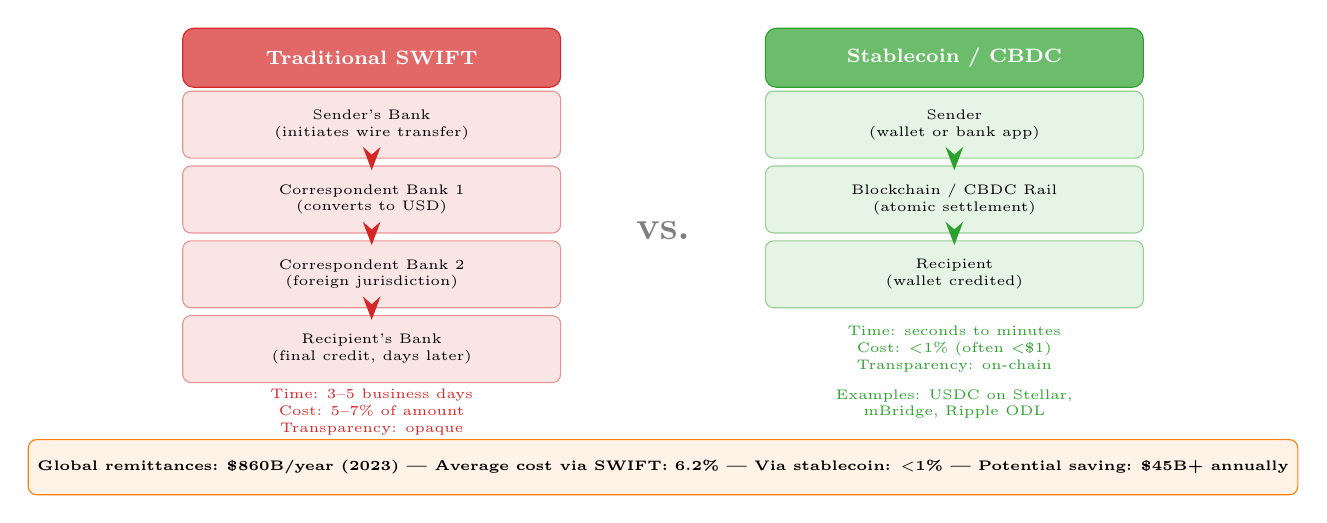
\begin{tikzpicture}
  %% Traditional (left column)
  \node[draw=mlred, fill=mlred!70, rounded corners=4pt, minimum width=4.8cm, minimum height=0.75cm, align=center, font=\scriptsize\bfseries, text=white] at (2.8,5.5) {Traditional SWIFT};
  \node[draw=mlred!50, fill=mlred!12, rounded corners=3pt, minimum width=4.8cm, minimum height=0.85cm, align=center, font=\tiny] at (2.8,4.65) {Sender's Bank\\(initiates wire transfer)};
  \node[draw=mlred!50, fill=mlred!12, rounded corners=3pt, minimum width=4.8cm, minimum height=0.85cm, align=center, font=\tiny] at (2.8,3.7) {Correspondent Bank 1\\(converts to USD)};
  \node[draw=mlred!50, fill=mlred!12, rounded corners=3pt, minimum width=4.8cm, minimum height=0.85cm, align=center, font=\tiny] at (2.8,2.75) {Correspondent Bank 2\\(foreign jurisdiction)};
  \node[draw=mlred!50, fill=mlred!12, rounded corners=3pt, minimum width=4.8cm, minimum height=0.85cm, align=center, font=\tiny] at (2.8,1.8) {Recipient's Bank\\(final credit, days later)};
  \node[font=\tiny, text=mlred, align=center] at (2.8,1.0) {Time: 3--5 business days\\Cost: 5--7\% of amount\\Transparency: opaque};

  \draw[-{Stealth}, very thick, mlred] (2.8,4.23) -- (2.8,4.07);
  \draw[-{Stealth}, very thick, mlred] (2.8,3.28) -- (2.8,3.12);
  \draw[-{Stealth}, very thick, mlred] (2.8,2.33) -- (2.8,2.17);

  %% Comparison divider
  \node[font=\Large\bfseries, text=mlgray] at (6.5,3.3) {vs.};

  %% Stablecoin/CBDC (right column)
  \node[draw=mlgreen, fill=mlgreen!70, rounded corners=4pt, minimum width=4.8cm, minimum height=0.75cm, align=center, font=\scriptsize\bfseries, text=white] at (10.2,5.5) {Stablecoin / CBDC};
  \node[draw=mlgreen!50, fill=mlgreen!12, rounded corners=3pt, minimum width=4.8cm, minimum height=0.85cm, align=center, font=\tiny] at (10.2,4.65) {Sender\\(wallet or bank app)};
  \node[draw=mlgreen!50, fill=mlgreen!12, rounded corners=3pt, minimum width=4.8cm, minimum height=0.85cm, align=center, font=\tiny] at (10.2,3.7) {Blockchain / CBDC Rail\\(atomic settlement)};
  \node[draw=mlgreen!50, fill=mlgreen!12, rounded corners=3pt, minimum width=4.8cm, minimum height=0.85cm, align=center, font=\tiny] at (10.2,2.75) {Recipient\\(wallet credited)};
  \node[font=\tiny, text=mlgreen, align=center] at (10.2,1.8) {Time: seconds to minutes\\Cost: $<$1\% (often $<$\$1)\\Transparency: on-chain};
  \node[font=\tiny, text=mlgreen, align=center] at (10.2,1.1) {Examples: USDC on Stellar,\\mBridge, Ripple ODL};

  \draw[-{Stealth}, very thick, mlgreen] (10.2,4.23) -- (10.2,4.07);
  \draw[-{Stealth}, very thick, mlgreen] (10.2,3.28) -- (10.2,3.12);

  %% Headline stat
  \node[draw=mlorange, fill=mlorange!10, rounded corners=3pt, minimum width=12.5cm, minimum height=0.7cm, align=center, font=\tiny\bfseries] at (6.5,0.3) {Global remittances: \$860B/year (2023) | Average cost via SWIFT: 6.2\% | Via stablecoin: $<$1\% | Potential saving: \$45B+ annually};
\end{tikzpicture}
\bottomnote{World Bank: remittances exceeded \$860B in 2023 | Stellar USDC: sub-second settlement, \$0.00001 fee | mBridge: live multi-CBDC corridor since 2022 | Ripple ODL (On-Demand Liquidity): XRP bridge for cross-border USD settlement}
\end{frame}

% Frame 54: The Future of Programmable Money
\begin{frame}{The Future of Programmable Money}
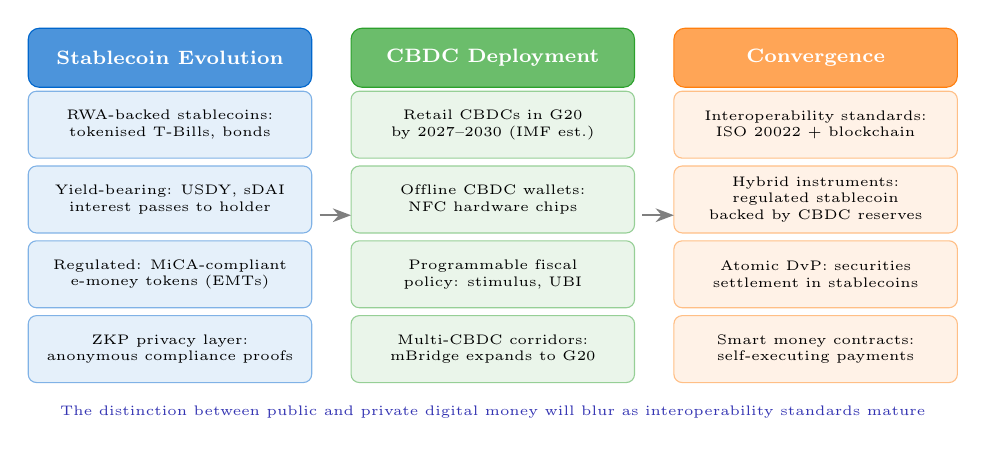
\begin{tikzpicture}
  %% Panel 1: Stablecoin Evolution
  \node[draw=mlblue, fill=mlblue!70, rounded corners=4pt, minimum width=3.6cm, minimum height=0.75cm, align=center, font=\scriptsize\bfseries, text=white] at (1.9,5.5) {Stablecoin Evolution};
  \node[draw=mlblue!50, fill=mlblue!10, rounded corners=3pt, minimum width=3.6cm, minimum height=0.85cm, align=center, font=\tiny] at (1.9,4.65) {RWA-backed stablecoins:\\tokenised T-Bills, bonds};
  \node[draw=mlblue!50, fill=mlblue!10, rounded corners=3pt, minimum width=3.6cm, minimum height=0.85cm, align=center, font=\tiny] at (1.9,3.7) {Yield-bearing: USDY, sDAI\\interest passes to holder};
  \node[draw=mlblue!50, fill=mlblue!10, rounded corners=3pt, minimum width=3.6cm, minimum height=0.85cm, align=center, font=\tiny] at (1.9,2.75) {Regulated: MiCA-compliant\\e-money tokens (EMTs)};
  \node[draw=mlblue!50, fill=mlblue!10, rounded corners=3pt, minimum width=3.6cm, minimum height=0.85cm, align=center, font=\tiny] at (1.9,1.8) {ZKP privacy layer:\\anonymous compliance proofs};

  %% Panel 2: CBDC Deployment
  \node[draw=mlgreen, fill=mlgreen!70, rounded corners=4pt, minimum width=3.6cm, minimum height=0.75cm, align=center, font=\scriptsize\bfseries, text=white] at (6.0,5.5) {CBDC Deployment};
  \node[draw=mlgreen!50, fill=mlgreen!10, rounded corners=3pt, minimum width=3.6cm, minimum height=0.85cm, align=center, font=\tiny] at (6.0,4.65) {Retail CBDCs in G20\\by 2027--2030 (IMF est.)};
  \node[draw=mlgreen!50, fill=mlgreen!10, rounded corners=3pt, minimum width=3.6cm, minimum height=0.85cm, align=center, font=\tiny] at (6.0,3.7) {Offline CBDC wallets:\\NFC hardware chips};
  \node[draw=mlgreen!50, fill=mlgreen!10, rounded corners=3pt, minimum width=3.6cm, minimum height=0.85cm, align=center, font=\tiny] at (6.0,2.75) {Programmable fiscal\\policy: stimulus, UBI};
  \node[draw=mlgreen!50, fill=mlgreen!10, rounded corners=3pt, minimum width=3.6cm, minimum height=0.85cm, align=center, font=\tiny] at (6.0,1.8) {Multi-CBDC corridors:\\mBridge expands to G20};

  %% Panel 3: Convergence
  \node[draw=mlorange, fill=mlorange!70, rounded corners=4pt, minimum width=3.6cm, minimum height=0.75cm, align=center, font=\scriptsize\bfseries, text=white] at (10.1,5.5) {Convergence};
  \node[draw=mlorange!50, fill=mlorange!10, rounded corners=3pt, minimum width=3.6cm, minimum height=0.85cm, align=center, font=\tiny] at (10.1,4.65) {Interoperability standards:\\ISO 20022 + blockchain};
  \node[draw=mlorange!50, fill=mlorange!10, rounded corners=3pt, minimum width=3.6cm, minimum height=0.85cm, align=center, font=\tiny] at (10.1,3.7) {Hybrid instruments:\\regulated stablecoin\\backed by CBDC reserves};
  \node[draw=mlorange!50, fill=mlorange!10, rounded corners=3pt, minimum width=3.6cm, minimum height=0.85cm, align=center, font=\tiny] at (10.1,2.75) {Atomic DvP: securities\\settlement in stablecoins};
  \node[draw=mlorange!50, fill=mlorange!10, rounded corners=3pt, minimum width=3.6cm, minimum height=0.85cm, align=center, font=\tiny] at (10.1,1.8) {Smart money contracts:\\self-executing payments};

  %% Arrows between panels
  \draw[-{Stealth}, thick, mlgray] (3.8,3.5) -- (4.2,3.5);
  \draw[-{Stealth}, thick, mlgray] (7.9,3.5) -- (8.3,3.5);

  \node[font=\tiny, text=mlpurple, align=center] at (6.0,1.0) {The distinction between public and private digital money will blur as interoperability standards mature};
\end{tikzpicture}
\bottomnote{BlackRock BUIDL: tokenised T-Bill fund; \$500M in 3 months | sDAI: MakerDAO savings rate; 5\%+ yield | BIS Project Mariana: automated FX using AMMs and wCBDCs | ISO 20022: global financial messaging standard adopted by SWIFT by 2025}
\end{frame}

% Frame 55: Key Takeaways and Course Summary
\begin{frame}{Key Takeaways and Course Summary}
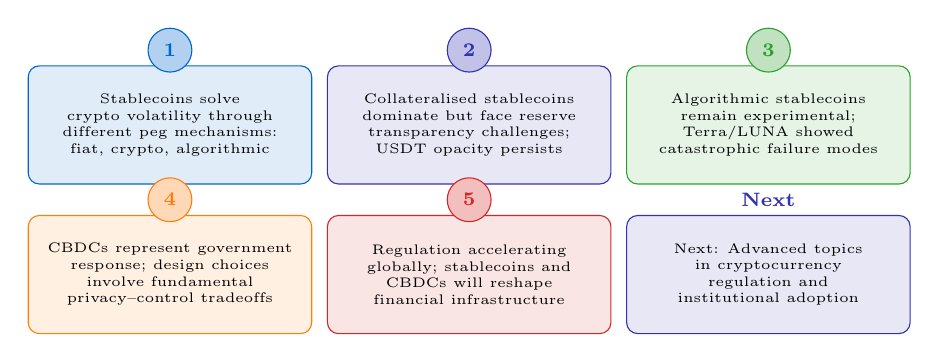
\begin{tikzpicture}
  \node[draw=mlblue, fill=mlblue!12, rounded corners=4pt, minimum width=3.6cm, minimum height=1.5cm, align=center, font=\tiny] (k1) at (1.9,3.2) {Stablecoins solve\\crypto volatility through\\different peg mechanisms:\\fiat, crypto, algorithmic};
  \node[circle, draw=mlblue, fill=mlblue!30, minimum size=0.55cm, font=\scriptsize\bfseries, text=mlblue] at (1.9,4.15) {1};

  \node[draw=mlpurple, fill=mlpurple!12, rounded corners=4pt, minimum width=3.6cm, minimum height=1.5cm, align=center, font=\tiny] (k2) at (5.7,3.2) {Collateralised stablecoins\\dominate but face reserve\\transparency challenges;\\USDT opacity persists};
  \node[circle, draw=mlpurple, fill=mlpurple!30, minimum size=0.55cm, font=\scriptsize\bfseries, text=mlpurple] at (5.7,4.15) {2};

  \node[draw=mlgreen, fill=mlgreen!12, rounded corners=4pt, minimum width=3.6cm, minimum height=1.5cm, align=center, font=\tiny] (k3) at (9.5,3.2) {Algorithmic stablecoins\\remain experimental;\\Terra/LUNA showed\\catastrophic failure modes};
  \node[circle, draw=mlgreen, fill=mlgreen!30, minimum size=0.55cm, font=\scriptsize\bfseries, text=mlgreen] at (9.5,4.15) {3};

  \node[draw=mlorange, fill=mlorange!12, rounded corners=4pt, minimum width=3.6cm, minimum height=1.5cm, align=center, font=\tiny] (k4) at (1.9,1.3) {CBDCs represent government\\response; design choices\\involve fundamental\\privacy--control tradeoffs};
  \node[circle, draw=mlorange, fill=mlorange!30, minimum size=0.55cm, font=\scriptsize\bfseries, text=mlorange] at (1.9,2.25) {4};

  \node[draw=mlred, fill=mlred!12, rounded corners=4pt, minimum width=3.6cm, minimum height=1.5cm, align=center, font=\tiny] (k5) at (5.7,1.3) {Regulation accelerating\\globally; stablecoins and\\CBDCs will reshape\\financial infrastructure};
  \node[circle, draw=mlred, fill=mlred!30, minimum size=0.55cm, font=\scriptsize\bfseries, text=mlred] at (5.7,2.25) {5};

  \node[draw=mlpurple, fill=mlpurple!12, rounded corners=4pt, minimum width=3.6cm, minimum height=1.5cm, align=center, font=\tiny] (k6) at (9.5,1.3) {Next: Advanced topics\\in cryptocurrency\\regulation and\\institutional adoption};
  \node[font=\scriptsize\bfseries, text=mlpurple] at (9.5,2.25) {Next};
\end{tikzpicture}
\bottomnote{Lecture complete: 55 frames | 5 sections | Key insight: digital money design is fundamentally about the trust triangle --- issuer, user, regulator | Further reading: BIS Annual Economic Report 2023, FSB stablecoin framework, ECB Digital Euro reports}
\end{frame}

\end{document}
